%!TEX TS-program = pdflatex
%!TEX encoding = UTF-8 Unicode
\documentclass[11pt,a4paper,english]{article}

\usepackage[utf8]{inputenc} %input chars
\usepackage[italian]{babel} %language
\usepackage[T1]{fontenc} %output chars
\usepackage{lmodern} %font
\usepackage{geometry} %page layout
\usepackage{amsfonts} %math symbols
\usepackage{amsmath} %math equations
\usepackage{amssymb} %math symbols
\usepackage{mathtools} %other math
\usepackage[numbers]{natbib} %bibliography
\usepackage[nottoc]{tocbibind} %other bib
\usepackage{paralist} %lists
\usepackage{graphicx}
\usepackage{subcaption}
\usepackage{multirow}
\usepackage{multicol}
\usepackage{pgfplots} %plots
\usepackage{listingsutf8}
\usepackage{epstopdf} %eps images
\usepackage{color} %colored text
\usepackage{algorithm2e}
\usepackage{float} %images going to end of the document
\usepackage{hyperref}
\usepackage[utf8]{inputenc} 
\usepackage{listings}
\makeatletter
\newcommand{\HEADER}[1]{\ALC@it\underline{\textsc{#1}}\begin{ALC@g}}
	\newcommand{\ENDHEADER}{\end{ALC@g}}
\makeatother
\usepackage{microtype} %better type
% questo sono i default per i listings 
\lstset{
	frame=tb, % draw a frame at the top and bottom of the code block
	tabsize=4, % tab space width
	showstringspaces=false, % don't mark spaces in strings
	breaklines=true,
	numbers=left, % display line numbers on the left
	basicstyle=\footnotesize,
	commentstyle=\color{gray}, % comment color
	keywordstyle=\color{blue}, % keyword color
	stringstyle=\color{red} % string color
}

\DeclareRobustCommand{\univsc}[1]{\Large\textsc{\textls[75]{#1}}}
\DeclareRobustCommand{\titlesc}[1]{\linespread{1.2}\LARGE{\textls[35]{\uppercase{#1}}\linespread{1}}}
\DeclareRobustCommand{\namesc}[1]{\large\textsc{\textls[35]{#1}}} 

\newcommand{\facciatabianca}{\newpage\shipout\null}

\lstset{defaultdialect=[Visual]Basic}

\allowdisplaybreaks

\begin{document}
	
\pagenumbering{Alph}
\begin{titlepage}
	
	\begin{center}
		\vbox to0pt{\vbox to\textheight{\vfil
{\tiny }				
\includegraphics[width=0.93\textwidth]{img/polloPallido.eps}\vfil}\vss}
	\end{center}
	
	\begin{center}  
		\univsc{Universit\`a degli Studi di Udine}
		\medskip   
		\rule{10cm}{.4pt}\\
		\medskip\begin{Large}
			\medskip
			\vspace{\stretch{0.6}}
			Tesi di Laurea Triennale in Informatica\end{Large}\\
		\medskip
		\vspace{\stretch{0.25}}
		\titlesc{Sviluppo di un sistema informatico per il gruppo di Protezione Civile di San Vito al Tagliamento}       % Inserire il titolo
		
		\bigskip\vfill
		\large
		\begin{tabular*}{\textwidth}{@{}l@{\extracolsep{\fill}}r@{}}
			\large Relatore:&Allievo:\\			% Eventualmente cambiare Allievo con Allieva. 
			% Relatore va lasciato invariato anche se è una donna.
			%  
			%Se il titolo onorifico del relatore è troppo lungo per stare sulla stessa riga (es:Chiar.mo Prof.)
			%cancellare il simbolo % nella riga qui sotto, sostituire i dati e inserire % all'inizio delle 2 righe sotto
			%Chiar.mo Prof.& \namesc{Nome studente}\\\namesc{Nome docente}&
			Prof.
			\namesc{Scagnetto Ivan}&% Inserire il nome del relatore. 
			% Se il relatore è un ricercatore sostituire Prof.\ con Dott.\
			% Se il relatore è una donna sostituire con Prof.ssa o Dott.ssa  															
			\namesc{Corrado Alessio}				% Inserire il proprio nome
			
		\end{tabular*}
		
	\end{center}
	
	\begin{center}
		\vfill
		\rule{10cm}{.4pt}\\
		\medskip
		\univsc{Anno Accademico 2020-21}\\  %verificare che l'anno accademico sia quello 
		%in cui si è seguito il corso su cui si è svolta la tesi 
	\end{center}	
	
\end{titlepage}

\newpage

\tableofcontents

\newpage
\pagenumbering{arabic}



\section{Introduzione}

\paragraph{} La Protezione Civile del comune di San Vito al Tagliamento \cite{protezionecivile} attualmente utilizza esclusivamente moduli cartacei per la gestione delle proprie attività, il tracciamento della partecipazione delle squadre e il mantenimento delle informazioni riguardanti il proprio inventario. 

\paragraph{} Lo scopo di questo progetto è la realizzazione di un sistema informatico che possa contribuire a migliorare l'efficienza, la sicurezza e la semplicità di gestione della parte burocratica. Inoltre, un'integrazione automatica dei dati e delle richieste migliora le capacità organizzative, in quanto semplifica la comunicazione tra i membri, rimuove l'onere dei capisquadra di ricordare precisamente tutte le informazioni necessarie (come l'elenco delle presenze e dei materiali) e fornisce una dashboard unica in cui è possibile visualizzare tutte le informazioni di cui si può aver bisogno. 

\paragraph{} In questa tesi verrà mostrato l'intero processo di sviluppo, a partire dal primo approccio con il committente e finendo con la pubblicazione del sistema. Verrà data particolare attenzione ai processi secondari e di gestione, i quali non producono software, ma sono necessari all'organizzazione interna del lavoro. Verranno anche presentati numerosi approfondimenti su processi e tecnologie specifiche applicati durante lo svolgimento del progetto. 





\section{Primo approccio}

\paragraph{} Il primo approccio consiste nella conoscenza reciproca tra committente e gruppo operativo. 

\paragraph{} Questa è una delle fasi più critiche perché da essa si determina la volontà di iniziare il progetto: si stabiliscono, a grandi linee, i requisiti che la soluzione dovrà avere, per capire quale sia la strada migliore affinché il committente possa risolvere il suo problema. Infatti, mettendo al primo posto la soddisfazione del cliente, non è scontato che la costruzione di un sistema informatico sia la soluzione migliore, né è scontato che il gruppo di lavoro disponga delle conoscenze e risorse adeguate allo sviluppo di tale sistema. 


\subsection{Raccolta dei requisiti esplorativa}

\paragraph{} Lo scopo della raccolta dei requisiti esplorativa è presentare al gruppo di lavoro il dominio applicativo\footnote{Il \emph{dominio applicativo} è il contesto in cui il sistema opera.} e il problema che si intende affrontare. Non è importante scendere nei dettagli: quello che è importante in questa fase è capire quale sia la soluzione ottimale per raggiungere la soddisfazione del cliente. 

\paragraph{} In genere viene effettuata mediante un singolo incontro preliminare, possibilmente di persona, tra un rappresentante del committente e il responsabile del gruppo operativo per quanto riguarda le relazioni esterne. Essendo molto sommaria, non necessita di una presenza massiccia, lasciando liberi gli altri membri del gruppo. 

\paragraph{} La discussione è informale e priva di schemi. Inizialmente il committente viene lasciato libero di presentare il contesto e le difficoltà attuali. Proseguendo nella conversazione, si chiede in linea generica quali siano le soluzioni precedenti che il cliente ha provato (se ce ne sono), quale sia la soluzione che il committente si immagina (se ce n'è una) e quali siano le sue aspettative su di essa. A questo punto il rappresentante del gruppo di lavoro dispone di abbastanza informazioni per poter formulare alcune soluzioni ipotetiche, e le presenta al committente, discutendone pregi e difetti. È importante concordare sull'ordine di grandezza di tempi, risorse e costi riguardanti il progetto, e se possibile elencare tutti i requisiti più stringenti (ad esempio la consegna rigorosamente entro una certa data, se richiesta). 

\paragraph{} Il tutto è effettuato in via approssimativa, quindi non è necessario avere conoscenze tecniche troppo specifiche. È però fondamentale che il rappresentante del gruppo operativo abbia conoscenze adeguate in modo da poter formulare soluzioni ragionevoli.

\paragraph{} Uno dei modi migliori di documentare l'incontro è scrivendo su carta in formato di appunti. È importante che siano sufficientemente comprensibili e coprano tutti gli argomenti affrontati. Un'altra tecnica è la registrazione dell'incontro, però rischia di mettere il committente a disagio, impedendogli di essere naturale e mettendogli timore di dire cose stupide. 


\begin{figure}[H]
    \centering
    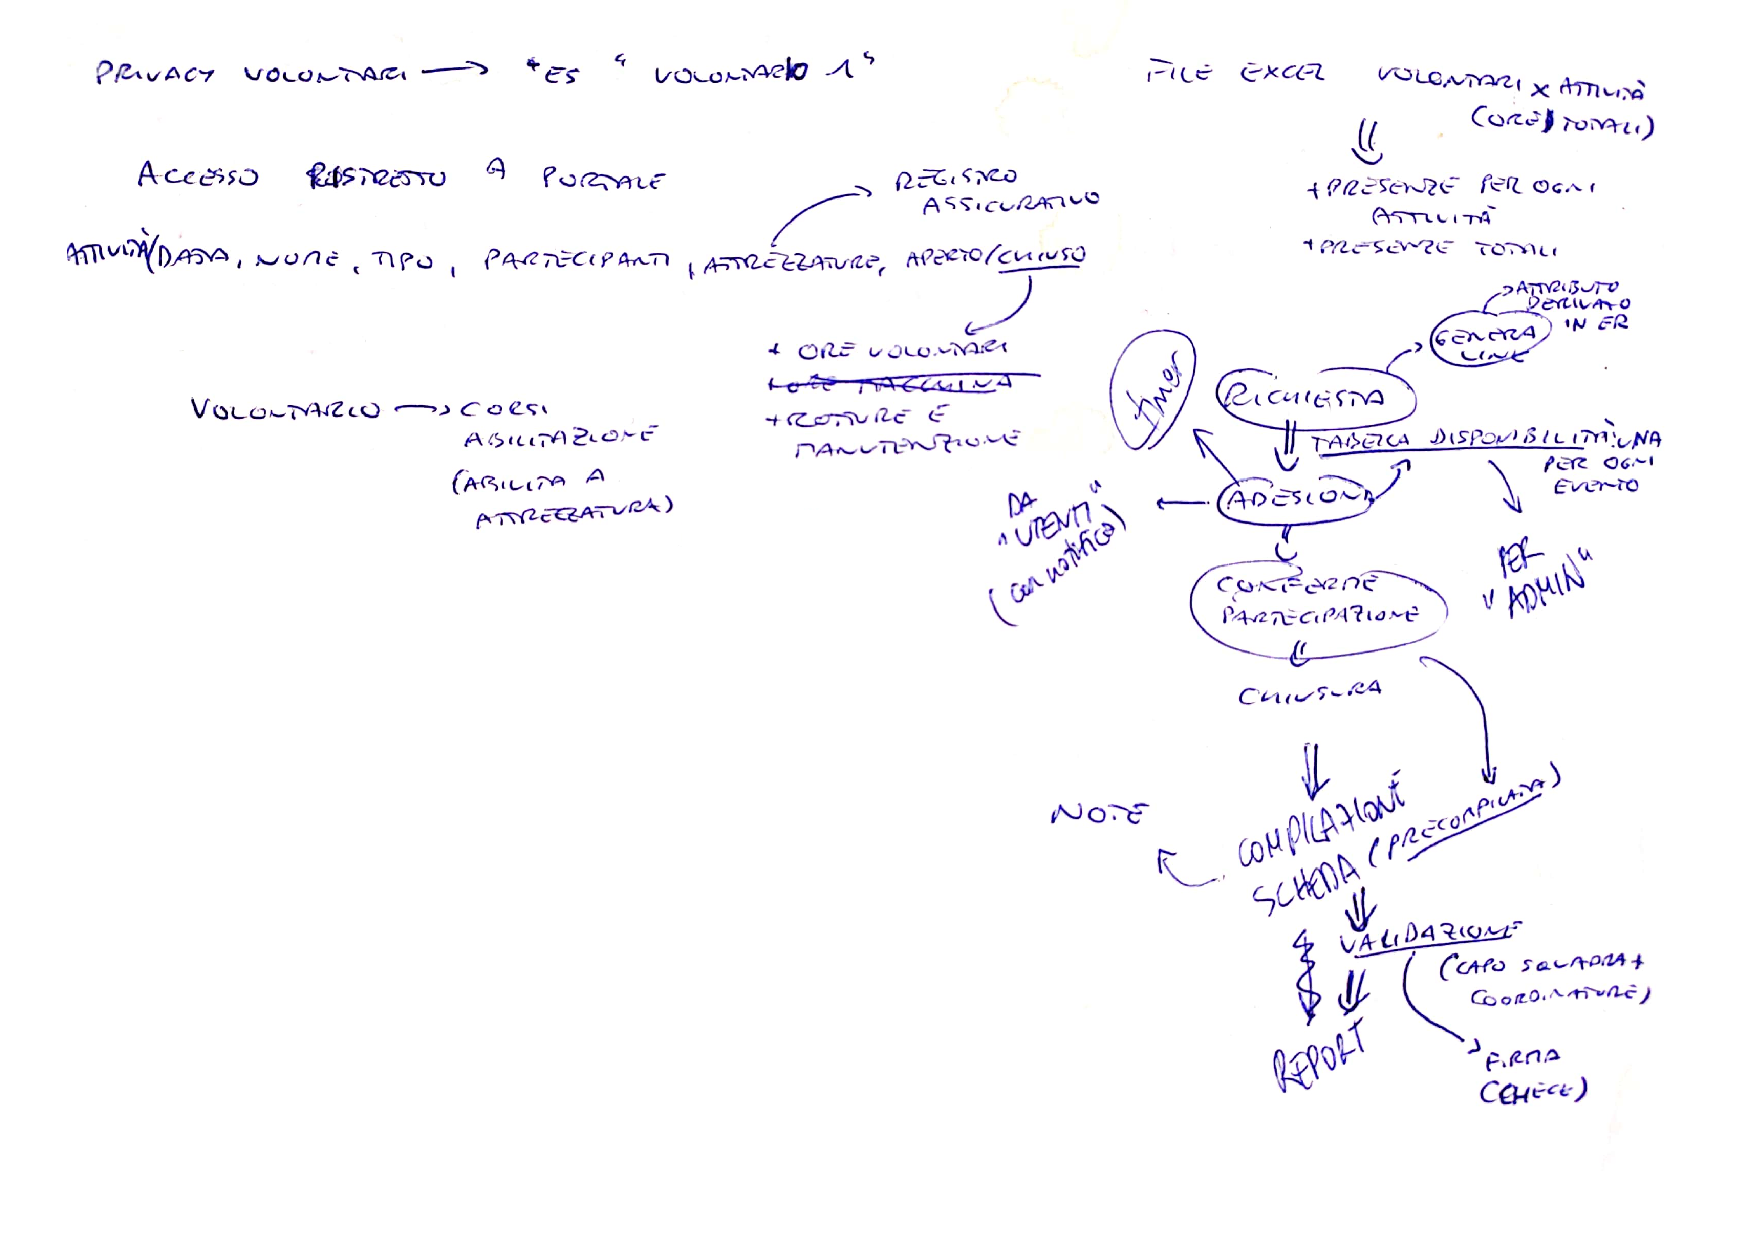
\includegraphics[width=1.0\textwidth]{img/analisi_esplorativa.pdf}
    \caption{Appunti della raccolta requisiti esplorativa}
\end{figure}


\subsection{Studio di fattibilità}

\paragraph{} Una volta completato l'incontro, il responsabile per le relazioni esterne si riunisce con l'intero gruppo di lavoro e presenta a tutti il progetto. 

\paragraph{} Il contributo tecnico altamente specifico di tutti i membri consente di effettuare, in primo luogo, lo studio di fattibilità ed una prima stima di tempi, costi e risorse. Infatti, in particolare nel caso di progetti svolti in gruppi ristretti, le richieste temporali e tecniche del progetto devono collimare con le disponibilità di tutti i membri del gruppo, altrimenti si rischia di ottenere un progetto incompleto.

\paragraph{} La modalità migliore di discussione è, ancora una volta, quella di effettuare un incontro "live". Una documentazione scritta richiederebbe un dispendio di tempo ed energie molto più elevato e non dà alcun vantaggio concreto. 

\paragraph{} Nel caso di questo progetto lo studio di fattibilità si è svolto in videoconferenza e ha prodotto i seguenti risultati:
\begin{itemize}
    \item Il progetto è completamente fattibile con tempi, risorse e costi adeguati.
    \item Il tempo di sviluppo indicativo è: 6 mesi.
    \item Non sono richieste risorse aggiuntive oltre quelle già presenti nel gruppo di lavoro.
    \item Non sono previsti particolari oneri finanziari a carico del committente o del gruppo di lavoro.
\end{itemize}

\paragraph{} Una volta svolto lo studio di fattibilità il committente viene contattato per informarlo dell'esito e, nel caso sia positivo, si conferma la volontà reciproca di proseguire nel progetto.


\subsubsection{Approfondimento: Come si valuta il successo?}

\paragraph{} Ci sono molti modi di definire il \emph{successo}. Ciò dipende sia dagli obiettivi personali, sia dal contesto in cui si parla. Alcuni esempi di caratteristiche del successo potrebbero essere: il profitto, la soddisfazione personale, il contributo ad una causa etica...

\paragraph{} Una definizione più formale di \emph{successo}, per quanto riguarda la creazione di un sistema informatico, è la seguente:

\paragraph{}
\emph{Svolgere il lavoro}
\begin{itemize}
    \item \emph{in time} e \emph{on schedule}: concludendo entro il tempo limite e rispettando la pianificazione;
    \item \emph{on budget}: rispettando i costi prestabiliti;
    \item in accordo con \emph{requirement} ed \emph{expectation}: deve fare quello che si era stabilito inizialmente, ma anche soddisfare le aspettative del committente;
    \item con un team felice: perché è importante che anche i membri del team siano contenti e soddisfatti del lavoro svolto! 
\end{itemize}

\paragraph{} Possiamo quindi vedere il successo non come un concetto unico, ma come la realizzazione di più obiettivi, che a volte possono persino essere contrastanti. Una delle maggiori difficoltà nel portare avanti un progetto è quella di trovare il giusto tradeoff per affrontare al meglio tutte le situazioni impreviste, in modo da trovare la conclusione migliore possibile. 






\section{Pianificazione iniziale}

\paragraph{} Per iniziare a lavorare sul progetto, è fondamentare decidere fin da subito quale sarà il modello di sviluppo adottato, in quanto esso ci dà gli stumenti per dividere il lavoro in task, organizzarli gerarchicamente e metterli in relazione tra loro  \cite{modelli_sviluppo, agile_manifesto}. 

\paragraph{} Le principali tipologie di modello sono: \emph{waterfall} e \emph{iterativo}. Nel modello \emph{waterfall} il processo di sviluppo si divide in fasi (requirements, specification, design, implementation, testing...) che vengono svolte in un ordine ben preciso, e gli output di una fase costituiscono l'input della sucessiva. Per dare inizio ad una fase bisogna attendere il completamento della precedente. Nei modelli \emph{iterativi} le fasi sono molto brevi e vengono ripetute iterativamente, in modo da aggiungere un po' alla volta nuove caratteristiche e funzionalità. Il modello waterfall fornisce migliori garanzie per quanto riguarda la prevedibilità, ma necessita di conoscere fin dall'inizio in modo preciso tutti i requisiti e pone molte difficoltà nel caso di cambiamenti in corso d'opera.

\begin{figure}[H]
    \centering
    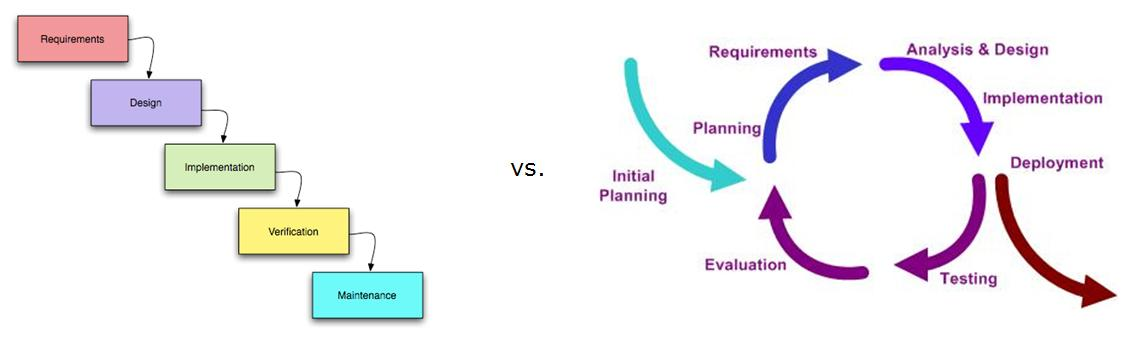
\includegraphics[width=1.0\textwidth]{img/waterfall_vs_iterativo.jpeg}
    \caption{Modello waterfall (a sinistra) vs iterativo (a destra)}
\end{figure}

\paragraph{} Una tecnica di supporto è il \emph{prototyping}: la costruzione di prototipi dimostrativi a basso costo che permettono la prova delle nuove funzionalità prima della loro effettiva implementazione. Il prototyping è molto utile quando si parte da specifiche incomplete (\emph{evolutionary prototyping}) oppure quando si vuole visualizzare un concetto nuovo (\emph{throw-away prototyping}). 

\begin{figure}[H]
    \centering
    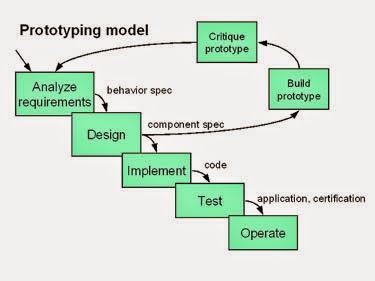
\includegraphics[width=0.4\textwidth]{img/prototyping.jpg}
    \caption{Introduzione del prototyping}
\end{figure}

\paragraph{} Il progetto nel generale utilizza una metodologia mista: c'è una sequenza di operazioni ben definita stile waterfall, in cui però le singole operazioni vengono ottimizzate con tecniche iterative e di prototyping. 

\begin{figure}[H]
    \centering
    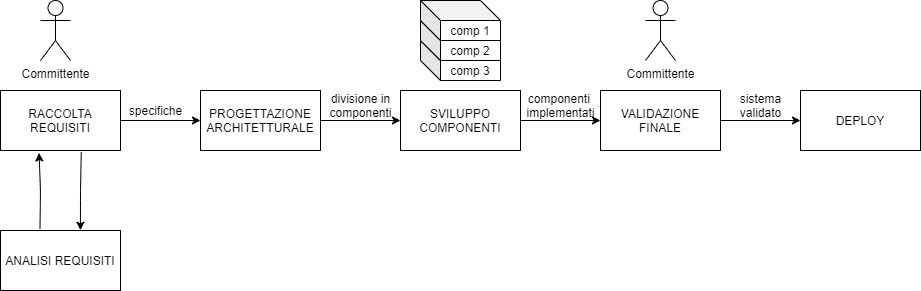
\includegraphics[width=1\textwidth]{img/pianificazione iniziale.png}
    \caption{Pianificazione iniziale}
\end{figure}


\section{Raccolta dei requisiti}

\paragraph{} La raccolta dei requisiti \cite{req_analysis} si prefigge di elencare \emph{precisamente} tutte le caratteristiche \emph {funzionali} e \emph{non funzionali}\footnote{Le caratteristiche funzionali legano gli input del sistema ai suoi output (ciò che il sistema fa). Le caratteristiche non funzionali sono molto più generiche e possono includere sia caratteristiche del sistema (ad esempio: tempi di risposta, tolleranza agli errori), sia vincoli esterni (ad esempio: legislativi, amministrativi, finanziari).} che il sistema dovrà avere. Questa fase serve per avere un'idea il più chiara possibile di quello che il committente vuole, in modo da \emph{minimizzare il rischio}\footnote{Si riferisce all'attività di \emph{risk management}} di produrre un sistema che non incontri le sue aspettative.

\subsection{Raccolta e analisi dei requisiti}

\paragraph{} La raccolta dei requisiti per il progetto è stata effettuata mediante una serie di incontri tra tutti i membri del gruppo di lavoro (in simultanea) e un membro responsabile/futuro utilizzatore del sistema per conto del committente. 

\paragraph{} Gli incontri, con il passare del tempo, sono diventati sempre più strutturati: mentre all'inizio era il committente a spiegare liberamente quelle che sono le sue richieste, poi erano i singoli membri del gruppo di lavoro a porre domande specifiche, mirate ad approfondire gli aspetti più critici per lo sviluppo del sistema. 

\paragraph{} Dopo il termine di ogni incontro sono stati organizzati dei meeting tra tutti i membri del team in modo da discutere, analizzare e sintetizzare quanto appreso, e di conseguenza preparare le domande per l'incontro successivo con il committente.


\begin{figure}[H]
    \centering
    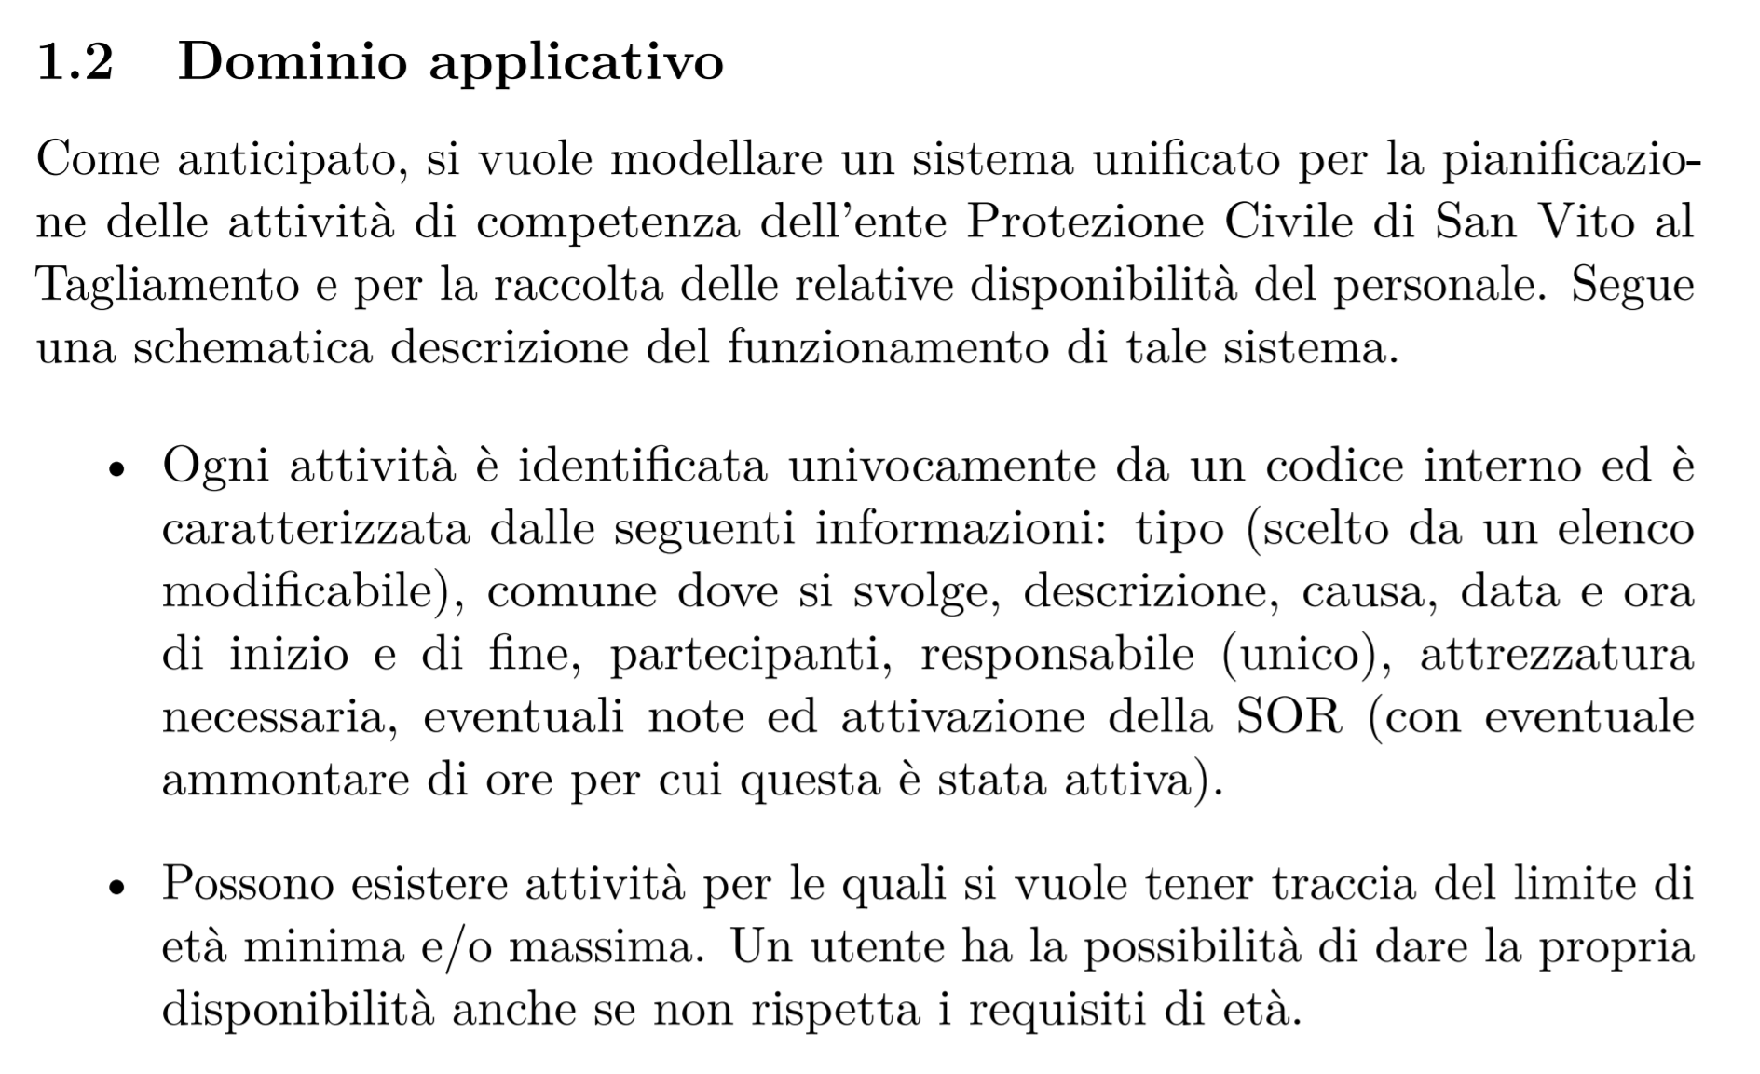
\includegraphics[width=0.7\textwidth]{img/requisiti_dominio.pdf}
    \caption{Parte del documento dei requisiti}
\end{figure}



\subsubsection{Approfondimento: Requisiti di qualità}

\paragraph{} Alla scrittura di requisiti di qualità viene spesso data poca importanza, in quanto vista come perdita di tempo poco utile ai fini dell'implementazione. Al contrario, il documento dei requisiti è il fulcro di tutta l'attività di sviluppo; infatti viene usato in ogni fase per capire cosa il committente \emph{vuole esattamente} dal sistema in produzione. 

\paragraph{} Il documento dei requisiti \cite{req_document} è l'input primario per la fase di definizione delle specifiche. Viene poi usato in fase di progettazione per sviluppare il sistema che meglio si adatta al committente e al contesto. È fondamentale per identificare le \emph{caratteristiche della qualità} importanti nel contesto di utilizzo. È utilizzato in fase di verifica per assicurarsi che il sistema faccia tutto ciò che deve (o non deve). Infine, può risultare tra i documenti legalmente vincolanti più influenti su cui si basa il contratto tra committente e sviluppatore. 

\paragraph{} Risulta quindi necessario avere un criterio oggettivo e sistematico per la creazione di requisiti di qualità. Un buon documento dei requisiti ha le seguenti caratteristiche:
\begin{itemize}
    \item \emph{correctness}: fornisce le funzionalità che supportano al meglio il committente;
    \item \emph{consistency}: non ci sono conflitti tra requisiti;
    \item \emph{completness}: sono incluse tutte le funzionalità richieste;
    \item \emph{comprensibility}: è facilmente comprensibile da tutti gli stakeholders;
    \item \emph{realism}: i requisiti sono fattibili;
    \item \emph{traceability}: si comprendono bene sia i collegamenti tra richieste e requisiti, sia i link inter-requisito;
    \item \emph{adaptability}: può essere modificato facilmente per venire incontro a nuove esigenze;
    \item \emph{verifiability}: i requisiti possono essere verificati in modo oggettivo.
\end{itemize}

\paragraph{} Il formato principale per il documento dei requisiti è testuale. Per questo è importante evitare ambiguità (la stessa parola ha significati diversi) e eccessiva flessibilità (lo stesso significato viene espresso con parole diverse). Un valido strumento in questi casi è il \emph{data dictionary}: un breve dizionario che spiega tutti i termini tecnici utilizzati e eventuali termini che possono risultare ambigui. 


\begin{figure}[H]
    \centering
    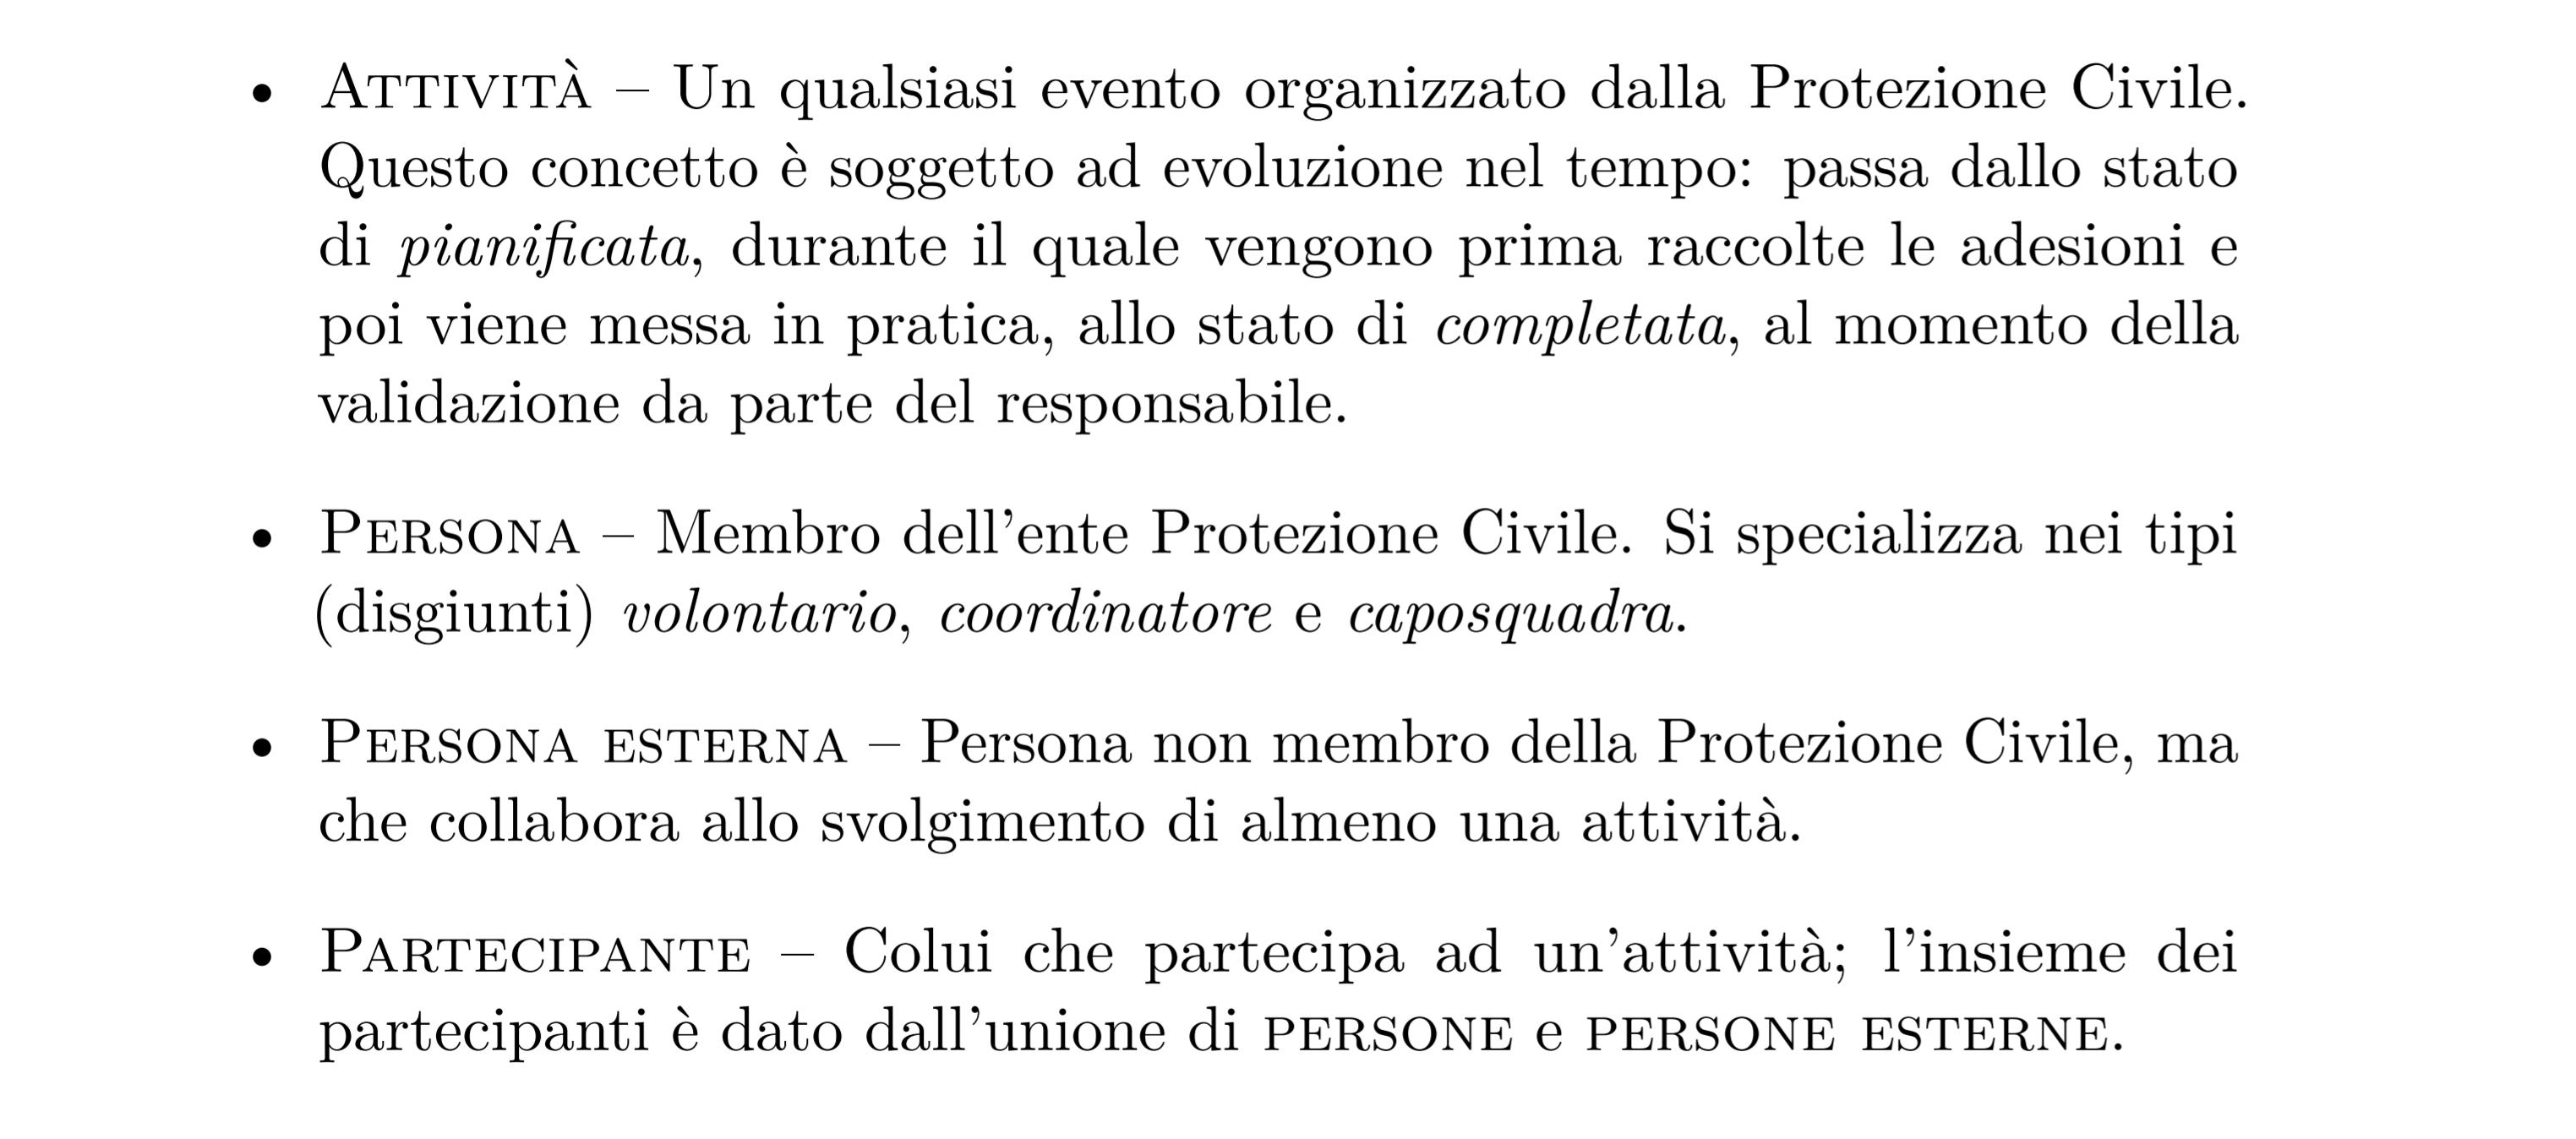
\includegraphics[width=0.8\textwidth]{img/data_dictionary.png}
    \caption{Frammento del data dictionary del progetto}
\end{figure}


\paragraph{} Per superare la linearità del linguaggio naturale è spesso utile utilizzare forme grafiche come: tabelle, flowchart, schemi, disegni, pseudolinguaggi... 

\paragraph{} Uno dei meccanismi per la verifica dei requisiti è la generazione di \emph{scenari}: si creano dei personaggi (stereotipi dei futuri utilizzatori), un contesto d'uso e una problematica che si vuole risolvere/azione da eseguire. Si fanno quindi interagire gli utenti con il sistema, in modo da mostrare al committente un esempio pratico di come il sistema si comporterà e verificare che faccia ciò che il committente si aspetta. Con l'utilizzo di \emph{prototipi} reali o in realtà virtuale, è possibile attuare gli scenari in modo da dare al committente un'esperienza ancora più realistica ed immersiva.



\subsubsection{Approfondimento: Risk management}

\paragraph{} L'attività di \emph{risk management} \cite{risk_management} si occupa di identificare i rischi e ideare piani per evitarli.

\paragraph{} Un \emph{rischio} è una probabilità dell'avvenimento di un evento negativo. Esso quindi è naturalmente caratterizzato da una \emph{probability} (very low < low < medium < high < very high) e da una \emph{severity} (insignificant < tolerable < serious < catastrophic). I rischi riguardano tutti gli aspetti del progetto: sia quelli strettamente legati all'implementazione, sia quelli interni al gruppo di lavoro, sia quelli esterni (legati al committente o indipendenti da esso). 

\paragraph{} Le fasi del risk management sono:
\begin{enumerate}
    \item \emph{risk identification}: fornisce una lista dei rischi (\emph{risk list});
    \item \emph{risk analysis}: assegna una priorità ai rischi (\emph{prioritized risk list});
    \item \emph{risk planning}: pianifica le azioni di contrasto ai rischi (\emph{risk avoidance} e \emph{contingency plan});
    \item \emph{risk monitoring}: monitora i rischi già identificati e l'insorgenza di nuovi (\emph{risk assessment}).
\end{enumerate}

\paragraph{} Le azioni intraprese dal risk management sono:
\begin{enumerate}
    \item \emph{avoidance}: riduce la probability del rischio;
    \item \emph{minimization}: riduce la severity del rischio;
    \item \emph{contingency}: attua contromisure al verificarsi del rischio.
\end{enumerate}

\begin{figure}[H]
    \centering
    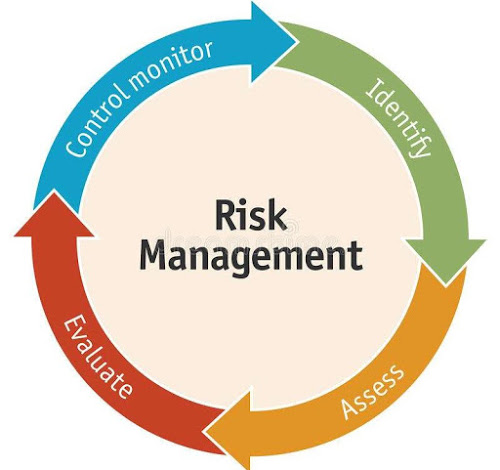
\includegraphics[width=0.6\textwidth]{img/risk_management.jpg}
    \caption{Processo di risk management}
\end{figure}

\paragraph{} È importante valutare tradeoff ottimali in modo che le azioni intraprese contro i rischi non abbiano controindicazioni peggiori dei rischi stessi (ad esempio, per minimizzare il rischio di produrre codice di bassa qualità si finisce per dilazionare troppo i tempi di implementazione e conseguentemente concludere in ritardo). 

\paragraph{} Il \emph{metodo a spirale} \cite{modelli_sviluppo} è un particolare metodo iterativo che basa le azioni da intraprendere sulla continua valutazione e minimizzazione dei rischi. 

\begin{figure}[H]
    \centering
    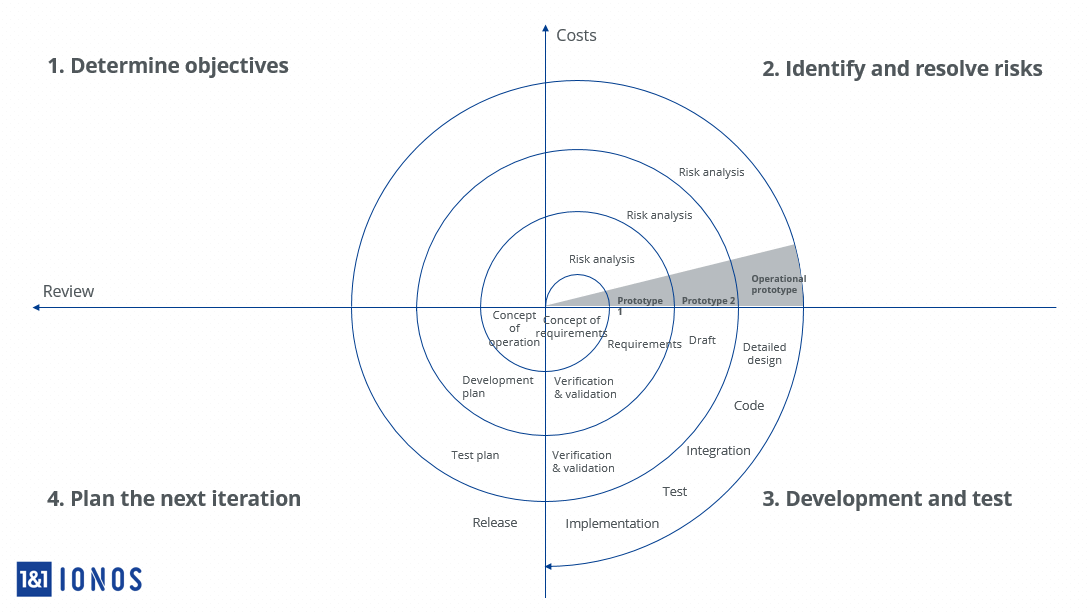
\includegraphics[width=1\textwidth]{img/modello_spirale.png}
    \caption{Modello a spirale}
\end{figure}




\section{Progettazione architetturale}

\paragraph{} Una volta raggiunto un documento dei requisiti soddisfacente, ha inizio una nuova fase: la \emph{progettazione architetturale} \cite{prog_architetturale}. 

\paragraph{} In questa fase si scompone il sistema in \emph{subsytems}, che poi verranno integrati per formare il sistema originale nella sua interezza. Questa scomposizione permette di concentrarsi su sottosistemi più semplici, riducendo quindi la complessità del problema. 

\paragraph{} Particolare attenzione in questa fase viene data al \emph{subsystem control and communication}. Esso consiste nella definizione delle strutture di controllo (chi controlla chi) e delle \emph{interfacce}\footnote{Un'\emph{interfaccia} è una definizione del "modo di comunicare" che ha un sistema. Solitamente è rappresentato da un insieme di metodi con relativa signature (nel paradigma a oggetti)} dei singoli sottosistemi.

\subsection{Architettura del sistema}

\paragraph{} Il nostro sistema si compone di quattro componenti:
\begin{itemize}
    \item \emph{Database}: si occupa di memorizzare i dati. Ha una piccola capacità di elaborazione: può ad esempio controllare che non ci siano duplicati o generare valori per nuovi inserimenti.
    \item \emph{Sito web}: utilizzato dagli amministratori per la parte di \emph{content management}\footnote{I \emph{content management systems}, per quanto riguarda i siti web, servono per gestire le impostazioni e i contenuti dei siti web lato amministrativo.} e in parte dagli utenti per una migliore consultazione di alcuni dati (es. analisi dei dati).
    \item \emph{Applicazione per smartphone}: utilizzato dagli utenti per interfacciarsi con il sistema.
    \item \emph{API web}: si frappone tra database e i client, in modo da implementare la logica del sistema. È anche il principale controllore della sicurezza (effettua l'autenticazione, protegge le risorse). 
\end{itemize}

\paragraph{} L'API web comunica direttamente con il database utilizzando una connessione, sia essa \emph{tcp} o \emph{unix socket}. Le richieste vengono inviate dall'API al database utilizzando il formato accettato dal database (SQL). 

\paragraph{} L'API web fornisce i propri servizi tramite protocollo \emph{REST}. I dati vengono codificati in formato \emph{JSON}. 

\paragraph{} L'app invia tutte le richieste all'API web. Non può dialogare direttamente con il database.

\paragraph{} Il browser ottiene le pagine web da un server web (statiche). All'interno delle pagine sono presenti degli \emph{script}\footnote{Gli \emph{script} sono piccoli programmi eseguibili, solitamente scritti in linguaggio JavaScript, che vengono eseguiti all'interno del browser e permettono la creazione di pagine web dinamiche.} che richiedono e inviano i dati all'API web. 

\paragraph{} Di seguito un \emph{diagramma di contesto}\footnote{I \emph{Data Flow Diagrams} sono particolari diagrammi, molto semplici ed intuitivi, utilizzati per spiegare con un approccio strutturato e funzionale quelli che sono i processi e i flussi di dati tra di essi. In particolare i DFD di livello 0 sono anche chiamati DFD di contesto.} \cite{dfd0} che mostra i flussi di comunicazione e controllo tra i sottosistemi.

\begin{figure}[H]
    \centering
    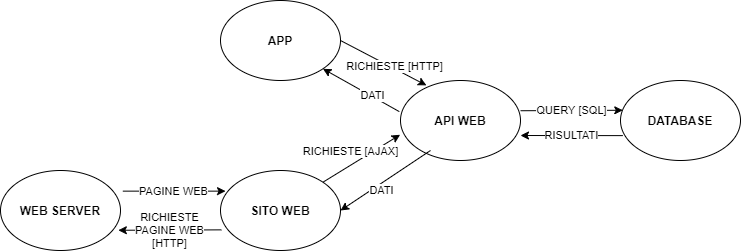
\includegraphics[width=1\textwidth]{img/architettura.png}
    \caption{Diagramma di contesto del sistema}
\end{figure}


\subsubsection{Approfondimento: Architettura REST e formato JSON}

\paragraph{} Il protocollo \emph{REST} \cite{rest} (Representational state transfer) è uno tra i più usati nella costruzione di \emph{web services}. 

\paragraph{} Esso sfrutta il protocollo \emph{HTTP}. Si basa sul concetto di \emph{risorsa}, identificata mediante un \emph{URI}, e di operazione, identificata da un tipo. Ad esempio, una richiesta \emph{"DELETE /persona/1234"} richiede la rimozione della persona con identificativo "1234".

\paragraph{} I dati, se presenti, vengono scritti nel \emph{body} HTTP (richiesta o risposta). Solitamente vengono formattati in un formato standard: HTML, JSON oppure XML. 

\begin{figure}[H]
    \centering
    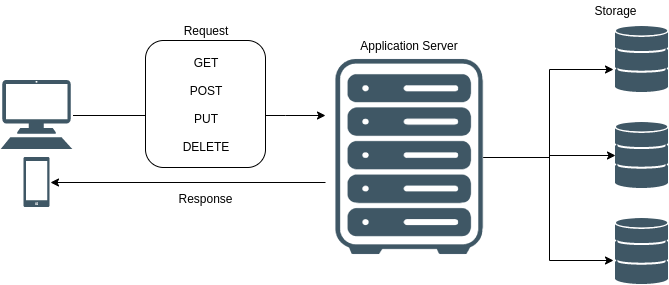
\includegraphics[width=0.8\textwidth]{img/rest.png}
    \caption{Struttura dell'architettura REST}
\end{figure}

\paragraph{} Il formato \emph{JSON} \cite{json} (JavaScript Object Notation) è uno tra i più usati per l'encoding di dati non primitivi. È estremamente semplice da leggere e scrivere, sia per l'umano che per un software. È molto più compatto di XML, rendendolo preferibile per l'utilizzo umano. È il formato usato per rappresentare gli oggetti nel linguaggio \emph{JavaScript}, e per questo risulta particolarmente familiare agli sviluppatori web. 

\begin{figure}[H]
    \centering
    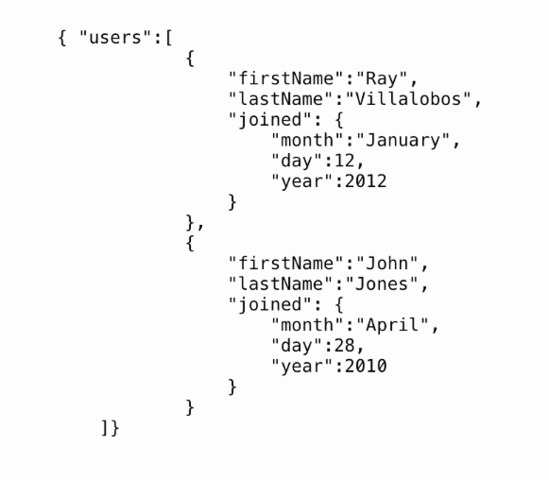
\includegraphics[width=0.6\textwidth]{img/json.jpeg}
    \caption{Esempio di file json}
\end{figure}


\subsection{Metodologia di lavoro}

\paragraph{} Una volta definita l'architettura del sistema, è necessario stabilire in che ordine e modo affrontare la progettazione e sviluppo dei singoli subsystems. 

\paragraph{} Dato che i subsystems individuati sono altamente indipendenti, il loro sviluppo potrebbe procedere in parallelo. Non avendo però necessità di terminare il progetto in tempi ristretti, risulta conveniente sviluppare prima il database, poi l'API, poi concorrentemente l'app e il website. In questo modo, è possibile evitare di sviluppare parte degli \emph{stub}\footnote{Gli \emph{stub} sono porzioni di codice che simulano la chiamata ad un modulo di livello inferiore. Sono utilizzati per il testing quando il modulo di livello inferiore non è ancora stato sviluppato.}, in quanto il modulo chiamato è già (in buona parte) implementato.

\paragraph{} Lo sviluppo verrà effettuato in modo incrementale. Il primo incremento sarà di grosse dimensioni, in modo da includere tutto quanto richiesto dal committente. Incrementi successivi verranno usati per effettuare le modifiche necessarie, individuate durante l'attività di validazione oppure non strettamente necessarie per avere un prototipo funzionante (ad esempio, la cifratura dei dati). 

\paragraph{} Il committente verrà costantemente tenuto aggiornato rispetto agli sviluppi del progetto. Ad ogni iterazione del ciclo di sviluppo, gli verrà mostrato quanto prodotto per procedere alla validazione. I suoi commenti verranno utilizzati come base per la pianificazione dell'incremento successivo.

\subsection{Stima dei tempi, costi e risorse}

\paragraph{} Avendo a disposizione molte più informazioni rispetto alla fase precedente, è possibile effettuare una migliore stima di tempi, costi e risorse. 

\paragraph{} La stima è la seguente:
\begin{itemize}
    \item \emph{Tempi}: 2 mesi per il database, 1 mese per l'API e 3 mesi per app+website, per quanto riguarda il primo e maggiore incremento. 
    \item \emph{Risorse}: I dispositivi propri del gruppo di sviluppo saranno sufficienti, almeno per quanto riguarda lo sviluppo. Per la validazione, potrà essere usato un qualche servizio di hosting cloud.
    \item \emph{Costi}: Per lo sviluppo, l'unico costo è quello della manodopera da parte del gruppo di lavoro. Essendo un progetto sviluppato a titolo gratuito, non sono previsti compensi per gli sviluppatori. Per la validazione, è previsto un massimo di euro 200 per quanto riguarda il servizio di cloud hosting. 
\end{itemize}

\paragraph{} Questo aggiornamento è stato subito comunicato al committente, per ragioni di trasparenza. 


\section{Qualità del software}

\paragraph{} Una nota particolare merita approfondimento: la qualità del software \cite{quality}. Essa non ha una definizione universale, ma va specificata di volta in volta.

\paragraph{} La qualità del software dipende dalle capacità degli sviluppatori e dalle caratteristiche del progetto. Per ottenere una maggiore qualità, risulta quindi necessario affidare il progetto a sviluppatori maggiormente specializzati e/o porre maggiore sforzo nello sviluppo. Il tutto si traduce in un aumento generale dei costi di sviluppo. 

\paragraph{} Inoltre, per garantire alcune caratteristiche minime (come la disponibilità), può essere necessario investire maggiori risorse finanziarie per l'acquisto di servizi di hosting.

\paragraph{} Non per tutti i progetti è necessario raggiungere la miglior qualità possibile: mentre sistemi \emph{life-critical}\footnote{I sistemi \emph{life-critical} sono quei sistemi da cui dipende la vita delle persone, come i sistemi medici o i sistemi di volo degli aerei.} devono garantire la miglior qualità possibile, sistemi di uso comune possono sacrificare parte della qualità in modo da ridurre tempi e costi. 

\paragraph{} Questo sistema deve avere le seguenti \emph{software characteristics}:
\begin{itemize}
    \item \emph{Availability}: buona. È auspicabile arrivare al 99\%. Una mancanza di disponibilità temporanea è sgradevole, ma non ha conseguenze catastrofiche. 
    \item \emph{Reliability}: ottima. Quando il sistema funziona, è importante che lo faccia senza malfunzionamenti. Dati errati potrebbero portare gli utilizzatori all'errore in condizioni critiche. È fortemente preferibile che il sistema non sia disponibile, piuttosto che funzioni in modo errato.
    \item \emph{Error tolerance}: ottima. Essendo un sistema utilizzato da persone non specializzate anche in condizioni di fretta, è importante ridurre al minimo la possibilità che un errore umano pregiudichi il funzionamento del sistema. 
    \item \emph{Recoverability}: ottima. In caso di malfunzionamento o errore umano, è importante conservare una copia dei dati integra. 
    \item \emph{Efficiency}: sufficiente. Il sistema deve rispondere in tempi ragionevoli, ma non è importante che sia particolarmente rapido. 
    \item \emph{Security}: ottima. Solo i membri autorizzati devono poter effettuare modifiche. Letture non autorizzate devono essere evitate, anche se il loro avvenimento non causa conseguenze particolarmente serie. 
    \item \emph{Suitability}: ottima. Essendo un sistema sviluppato per un committente specifico, è importante che offra le funzionalità per lui migliori. 
    \item \emph{Learnability}: buona. Deve poter essere compreso da tutti, anche chi non ha specifiche competenze informatiche, in modo da incoraggiarne l'utilizzo. Si tollera un tempo di apprendimento iniziale.
    \item \emph{Operability}: ottima. Una volta che l'utente ha imparato ad utilizzare il sistema, deve poterlo utilizzare sul campo in modo veloce e senza introdurre stress.
\end{itemize}


\subsubsection{Approfondimento: Qualità del software}

\paragraph{} Secondo la definizione \emph{ISO}\footnote{L'\emph{International Organization for Standardization} è un ente che si propone di formulare standard per l'utilizzo mondiale sulle materie più disparate.}:
\begin{quote}
    La \emph{software quality} è la totalità delle features e caratteristiche del prodotto software legate alla sua abilità di soddisfare necessità/bisogni/aspettative scritte o implicite.
\end{quote}

\paragraph{} La \emph{ISO 9000 series} contiene le guideline riguardanti \emph{quality management} e \emph{quality assurance}. In particolare, \emph{ISO 9000-3} si occupa dell'applicazione di \emph{ISO 9001} per lo sviluppo, fornitura e manutenzione del software. 

\paragraph{} Il processo di \emph{quality assurance} è il processo generale relativo all'organizzazione attuata per raggiungere i requisiti di qualità contenuti nella \emph{quality policy}. Il processo di \emph{quality control} è composto dalle tecniche specifiche e attività svolte nel \emph{quality system} per soddisfare i \emph{quality requirements} del singolo progetto. In particolare, le \emph{quality review} sono le azioni specifiche che valutano uno o più quality requirement. 

\paragraph{} La \emph{ISO 9000 certification} viene assegnata da particolari commissioni di valutazione alle società che dimostrano di comprendere ed applicare le norme ISO nel loro operato. Essa è una delle cerificazioni più importanti e di valore per dimostrare ai propri clienti di applicare elevati standard di qualità.

\paragraph{} Le \emph{software quality characteristics} sono gli attributi di un software product la cui qualità è descritta e valutata. 

\paragraph{} Una \emph{software quality metric} specifica la scala quantitativa e il metodo utilizzati per determinare oggettivamente il valore di una software quality characteristic. 

\paragraph{} Un \emph{software quality model} è un insieme di software quality characreristics, che viene utilizzato per valutare la qualità di un software. Esso dipende fortemente dalle caratteristiche del software e del contesto d'uso. 

\paragraph{} \emph{ISO/IEC WD 9126-1} elenca e definisce in modo completo le caratteristiche applicabili ad un software quality model. Esse sono divise in tre grandi gruppi: \begin{itemize}
    \item \emph{External characteristics}: valutate durante l'esecuzione.
    \item \emph{Internal characteristics}: valutate mediante \emph{software inspections}.
    \item \emph{In use characteristics}: effetti dell'uso del software in un contesto specifico.
\end{itemize}

\begin{figure}[H]
    \centering
    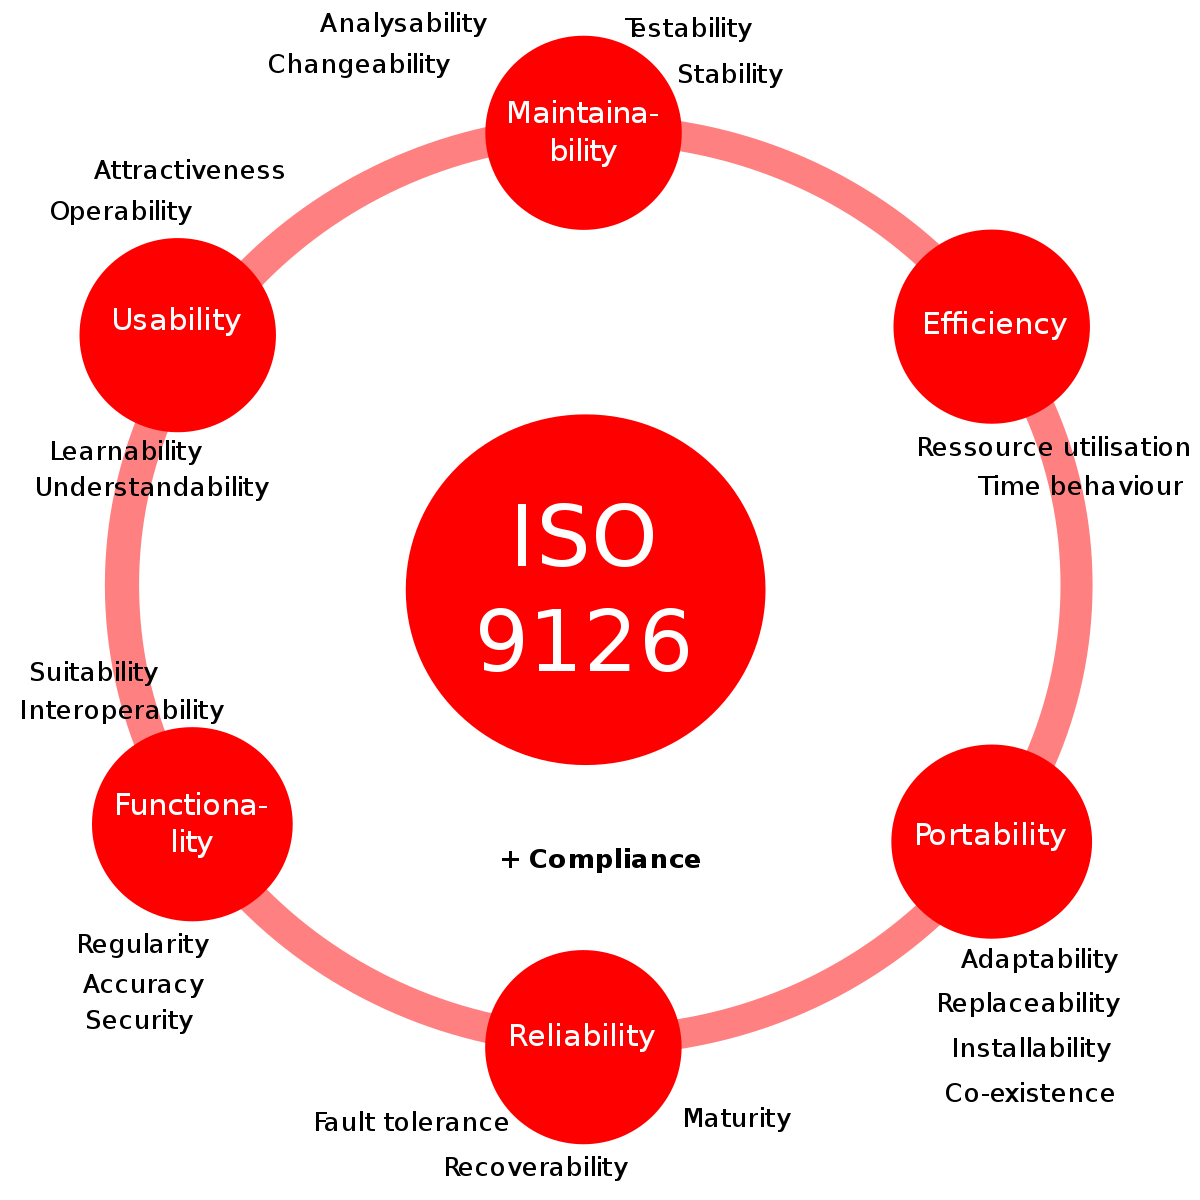
\includegraphics[width=0.8\textwidth]{img/iso_9126.png}
    \caption{Caratteristiche della qualità}
\end{figure}

\paragraph{} L'adozione di questi standard, anche senza disporre della certificazione, permette di avere strumenti oggettivi con cui valutare il proprio operato e poter fornire un prodotto di ottima qualità.


\subsubsection{Approfondimento: Testing}

\paragraph{} Per valutare le caratteristiche della qualità, nonché per verificare il corretto funzionamento del sistema, lo strumento principale utilizzato è il testing \cite{testing}. 

\paragraph{} Esso permette di \emph{verificare} e \emph{valutare}\footnote{La \emph{verifica} è il processo che compara il software con le specifiche, in modo da individuare errori di programmazione e controllare che il software faccia \emph{quanto stabilito} ("stiamo costruendo bene il sistema richiesto?"). La \emph{validazione} invece controlla che il software incontri davvero le \emph{necessità del committente}, anche se esse dovessero discostarsi dai requisiti ("stiamo costruento il sistema giusto per il committente?").} il sistema durante tutte le fasi, dalla progettazione alla consegna. 

\paragraph{} La principale distinzione tra tipologie di testing è tra \emph{software inspections} e \emph{verifiche in esecuzione}. Le prime consistono nell'esaminazione diretta del codice da parte di un programmatore, e quindi possono essere eseguite durante tutto il ciclo di vita. Le verifiche in esecuzione sono eseguite valutando la risposta del sistema a particolari input, e quindi necessitano di avere un eseguibile funzionante.

\paragraph{} Il \emph{component testing} si occupa del testing di un singolo componente, o sottosistema. L'\emph{integration testing} testa invece le interazioni tra i componenti, mettendoli assieme. Affinché l'integration testing abbia successo, è necessario prima aver verificato il funzionamento di tutti i componenti. 

\paragraph{} Il \emph{black-box testing} inventa i casi di test guardando solamente le specifiche. I \emph{testcase}\footnote{I \emph{testcase} sono coppie, in cui ad un input viene associato il comportamento del sistema che ci si aspetta con quell'input.} In genere si controllano alcuni input "normali" e alcuni input "anormali". Particolare attenzione viene data ai \emph{corner case}. 

\paragraph{} Il \emph{white-box testing} invece deriva i testcase dal codice. Si tenta di eseguire ogni linea di codice, dando particolare attenzione alle strutture di controllo (come condizioni e cicli). A riguardo, il \emph{path testing} studia i testcase in modo da eseguire una volta tutti i possibili cammini nel codice. 

\paragraph{} L'\emph{interface testing} prova a dialogare con un componente tramite le sue interfacce. Si dà importanza all'utilizzo in modo corretto delle interfacce (\emph{interface misusing}), alle assunzioni che il chiamante fa riguardo all'interfaccia (\emph{interface misunderstanding}) e all'interazione tra componenti con velocità diverse (\emph{timing errors}).

\paragraph{} La tecnica del \emph{regression testing} consiste nell'effettuare, ad ogni incremento, tutti i test precedenti, per verificare di non aver introdotto difetti.

\paragraph{} Lo \emph{stress test} carica il sistema o una parte oltre il suo limite in modo da verificarne il funzionamento e il degrado delle performance.

\paragraph{} Per effettuare i test spesso è necessario utilizzare degli \emph{stub} o \emph{test driver}. Gli stub sono parti di codice che simulano moduli di livello inferiore (chiamati), mentre i test driver simulano moduli di livello superiore (chiamanti).

\paragraph{} Il \emph{validation testing} viene usato al termine dello sviluppo per validare il software, e decidere se sono necessarie modifiche o si può consegnare. Il modo migliore per svolgerlo è far provare il sistema da quelli che saranno gli utilizzatori finali per un congruo lasso di tempo e senza dare indicazioni (perché poi nell'effettivo utilizzo non saranno seguiti dal vivo). 

\begin{figure}[H]
    \centering
    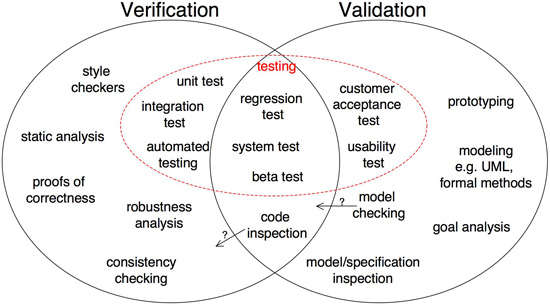
\includegraphics[width=0.8\textwidth]{img/verifica_validazione.jpg}
    \caption{Verifica e validazione}
\end{figure}



\section{Database}

\paragraph{} In questa sezione verrà presentato lo sviluppo del database \cite{db}, prima azione compiuta a seguito della progettazione architetturale. Tutti gli altri sottosistemi dipendono da esso, quindi durante la progettazione è stato necessario tenere in considerazione le esigenze di essi.

\subsection{Progettazione concettuale}

\paragraph{} Il primo passaggio nella progettazione di una base di dati è la \emph{progettazione concettuale}. Essa si basa sui requisiti e produce una prima rappresentazione del contenuto della base di dati, svincolata dalla sua effettiva implementazione. Il suo risultato è lo \emph{schema Entità-Relazioni}. 

\begin{figure}[H]
    \centering
    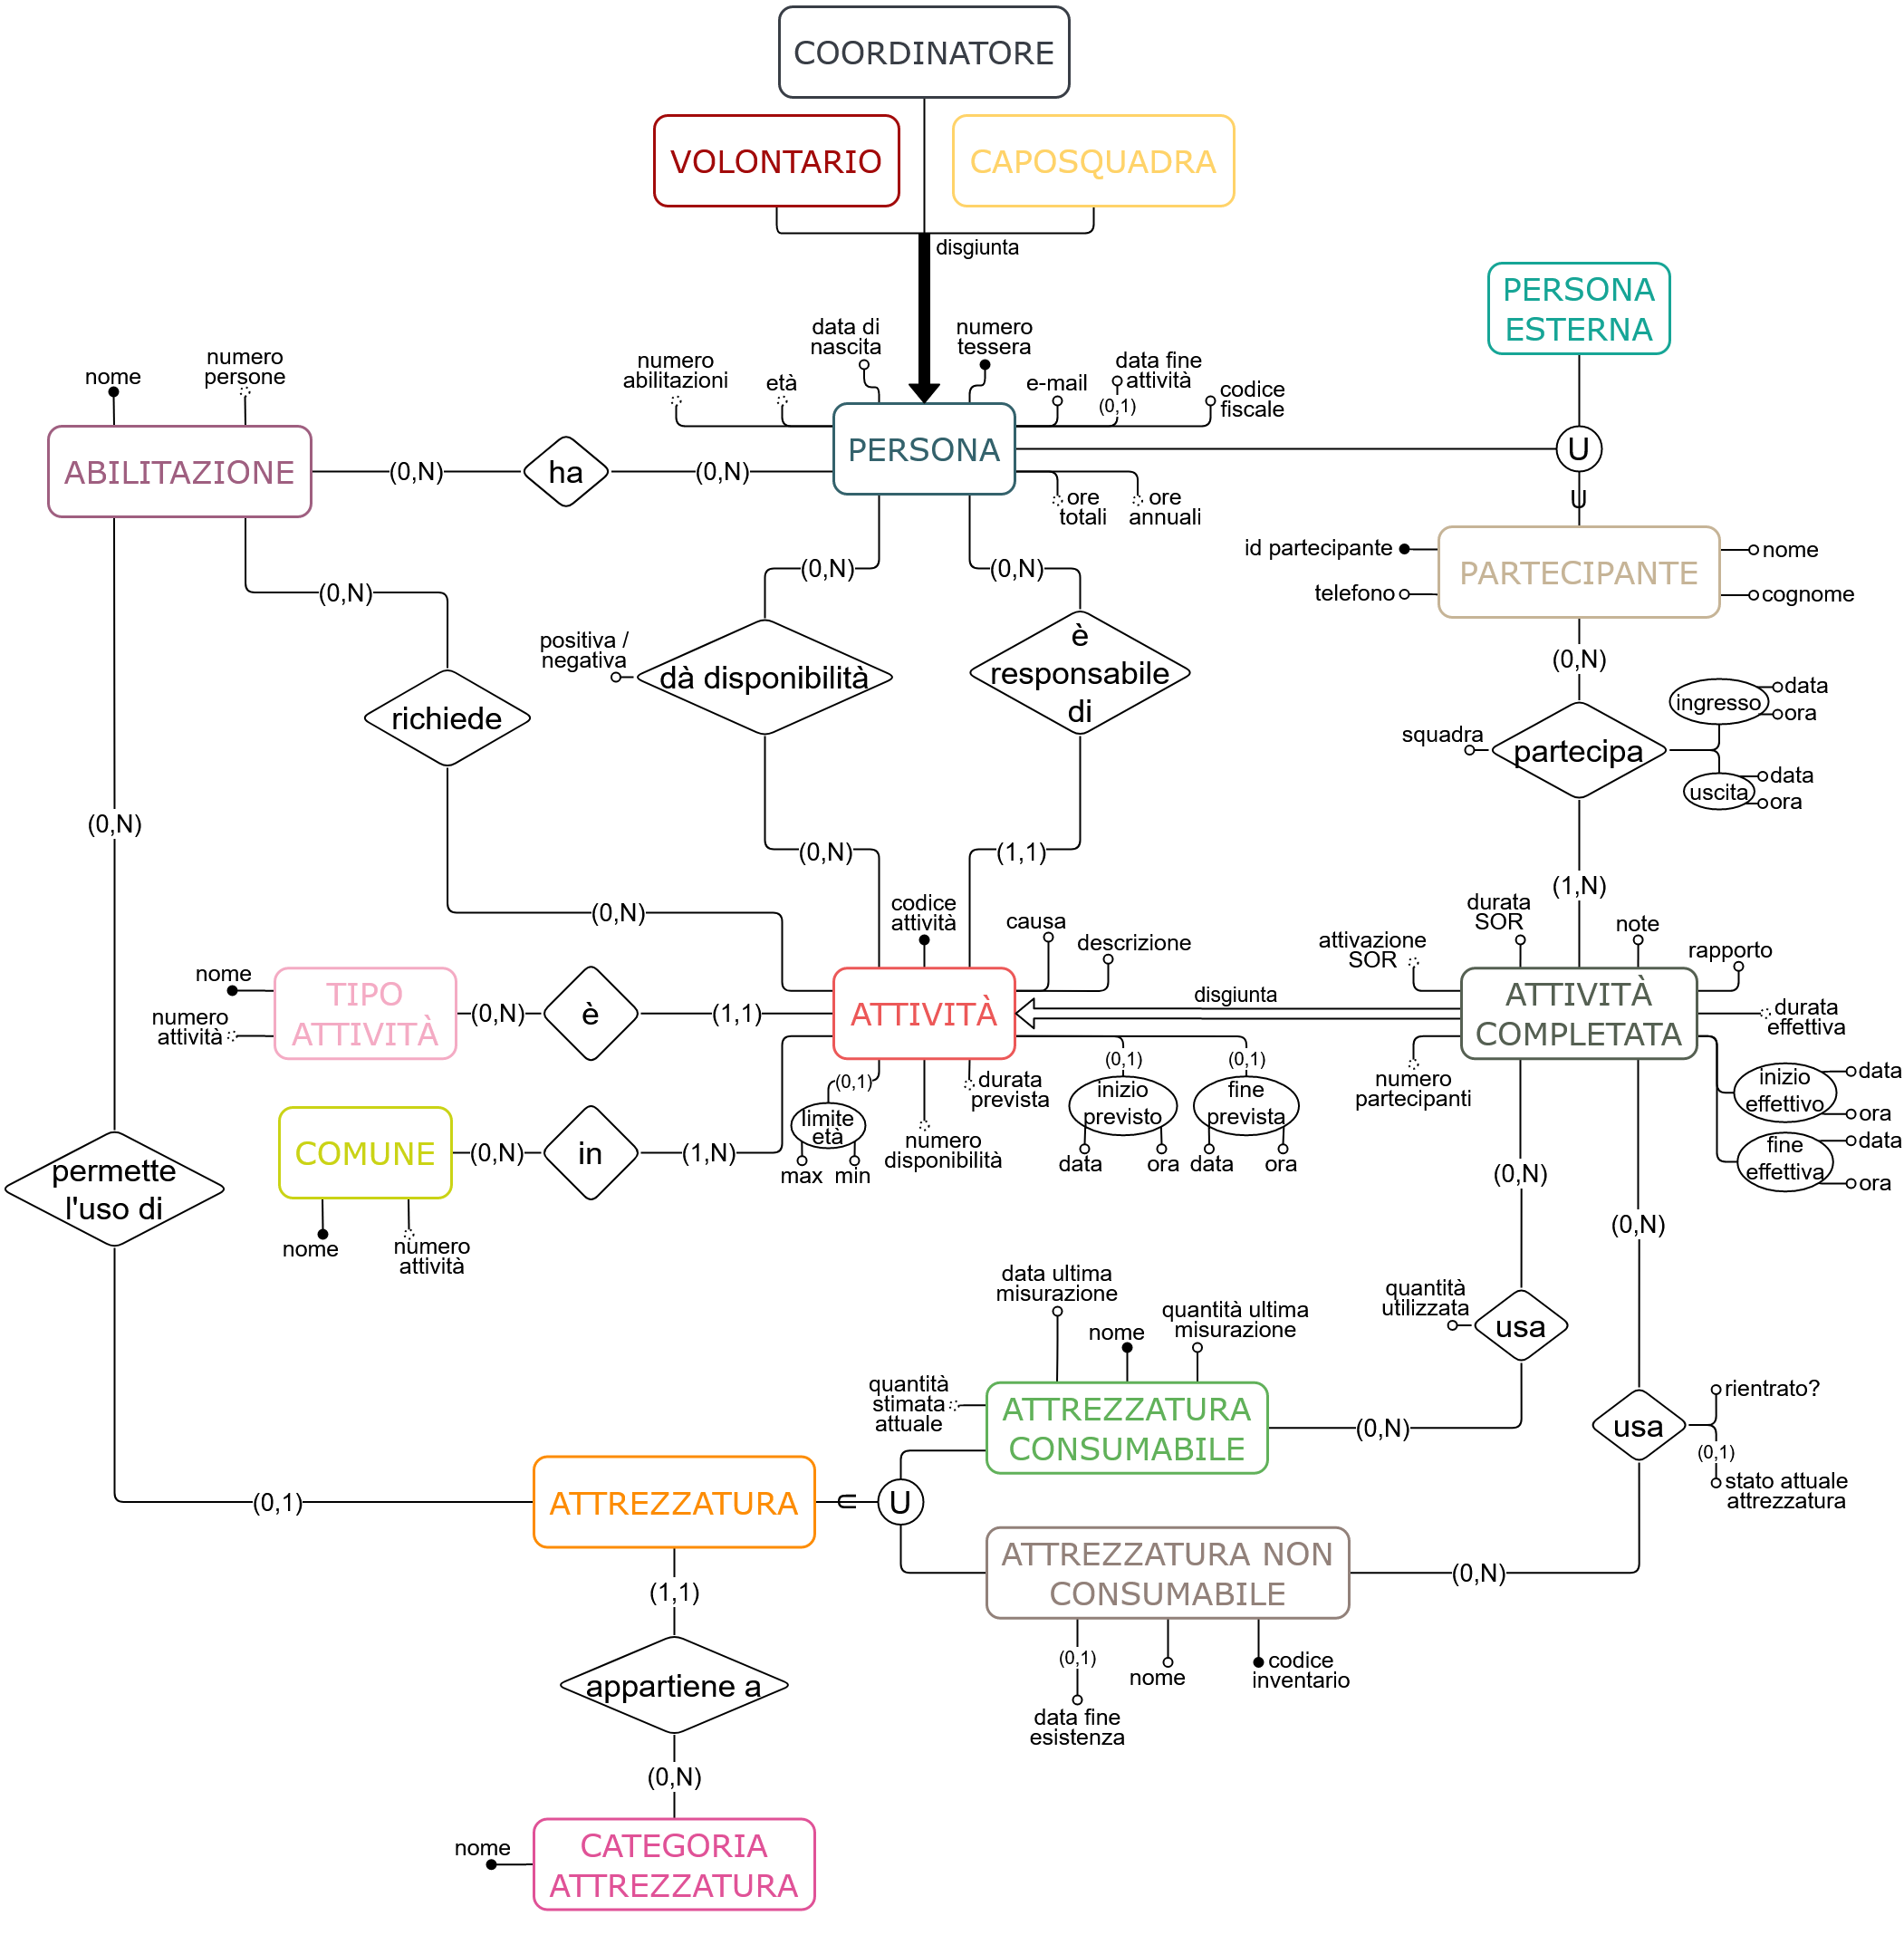
\includegraphics[width=1\textwidth]{img/er-schema.png}
    \caption{Schema ER}
\end{figure}

\paragraph{} Per modellare la base di dati, si è scelto di utilizzare il modello \emph{relazionale}, in quanto la base di dati è fortemente strutturata.

\subsection{Progettazione logica}

\paragraph{} Tutte le relazioni di tipo \emph{N a N}, non essendo direttamente rappresentabili nel modello relazionale, sono state reificate introducendo adeguate entità intermedie. Al termine di ciò, tutte le relazioni presenti sono di tipologia \emph{1 a N} oppure \emph{1 a 1}. 

\begin{figure}[H]
    \centering
    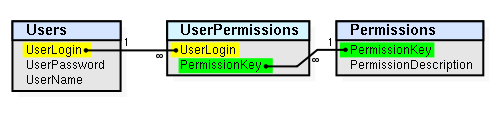
\includegraphics[width=0.8\textwidth]{img/junction_table.png}
    \caption{Esempio di tabella associativa usata per modellare una relazione N a N}
\end{figure}

\paragraph{} A seguito è stata eseguita l'\emph{analisi delle ridondanze}. Essa prende in input lo schema ER, la \emph{tabella delle frequenze}\footnote{La \emph{tabella delle frequenze} stima la frequenza di esecuzione delle principali operazioni sulla base di dati.} e la \emph{tabella dei volumi}\footnote{La \emph{tabella dei volumi} stima il numero di istanze per ciascuna entità e ciascuna relazione presenti nella base di dati.} per produrre un insieme di \emph{tabelle degli accessi}. Esse permettono, per ogni ridondanza, di scegliere se risulti computazionalmente conveniente mantenerla o eliminarla. 

\begin{figure}[H]
    \centering
    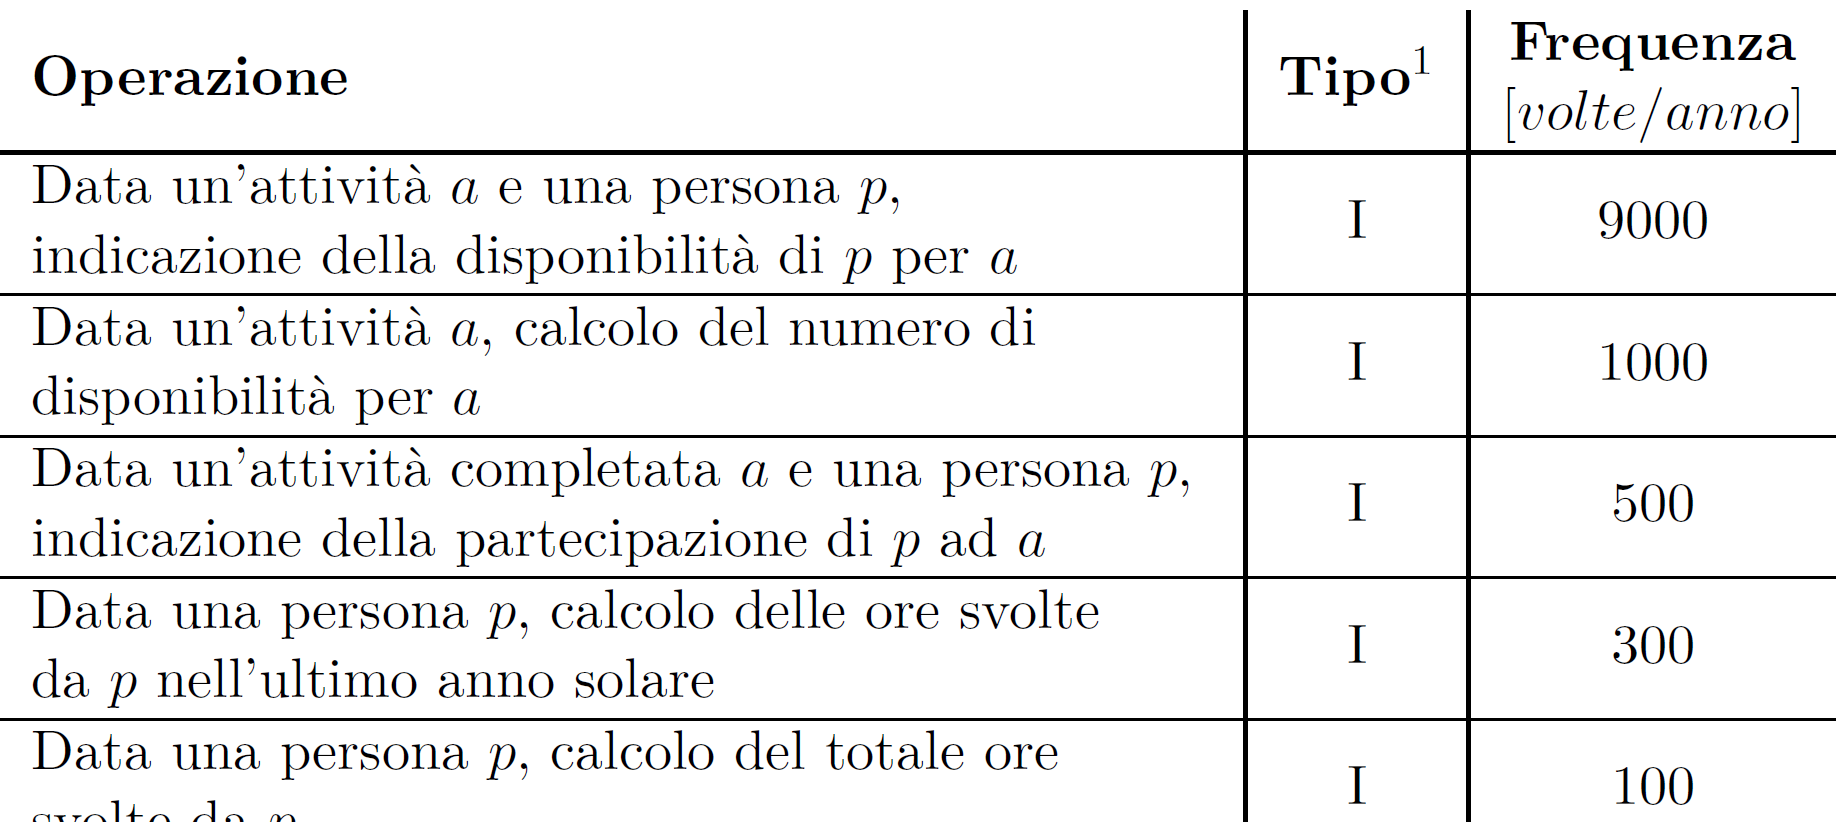
\includegraphics[width=0.6\textwidth]{img/tab_frequenze.png}
    \caption{Frammento della tabella delle frequenze}
\end{figure}

\begin{figure}[H]
    \centering
    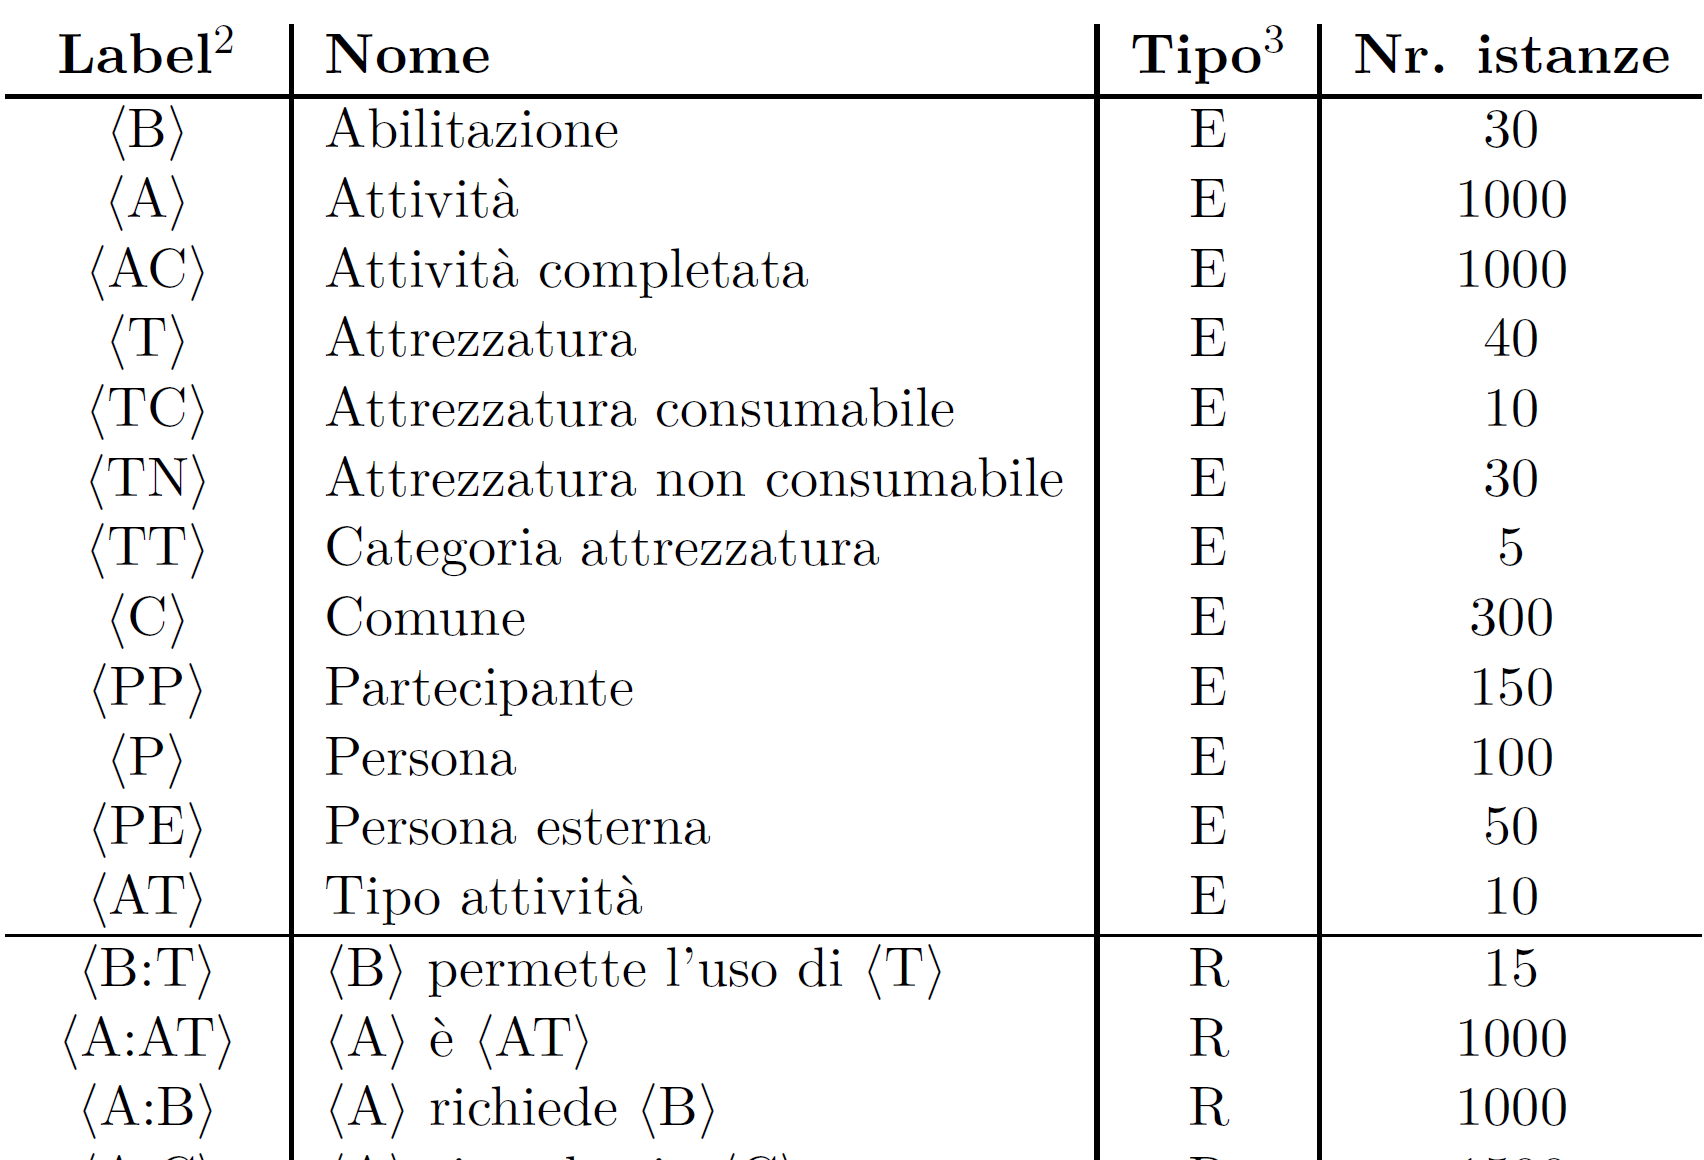
\includegraphics[width=0.6\textwidth]{img/tab_volumi.png}
    \caption{Frammento della tabella dei volumi}
\end{figure}

\begin{figure}[H]
    \centering
    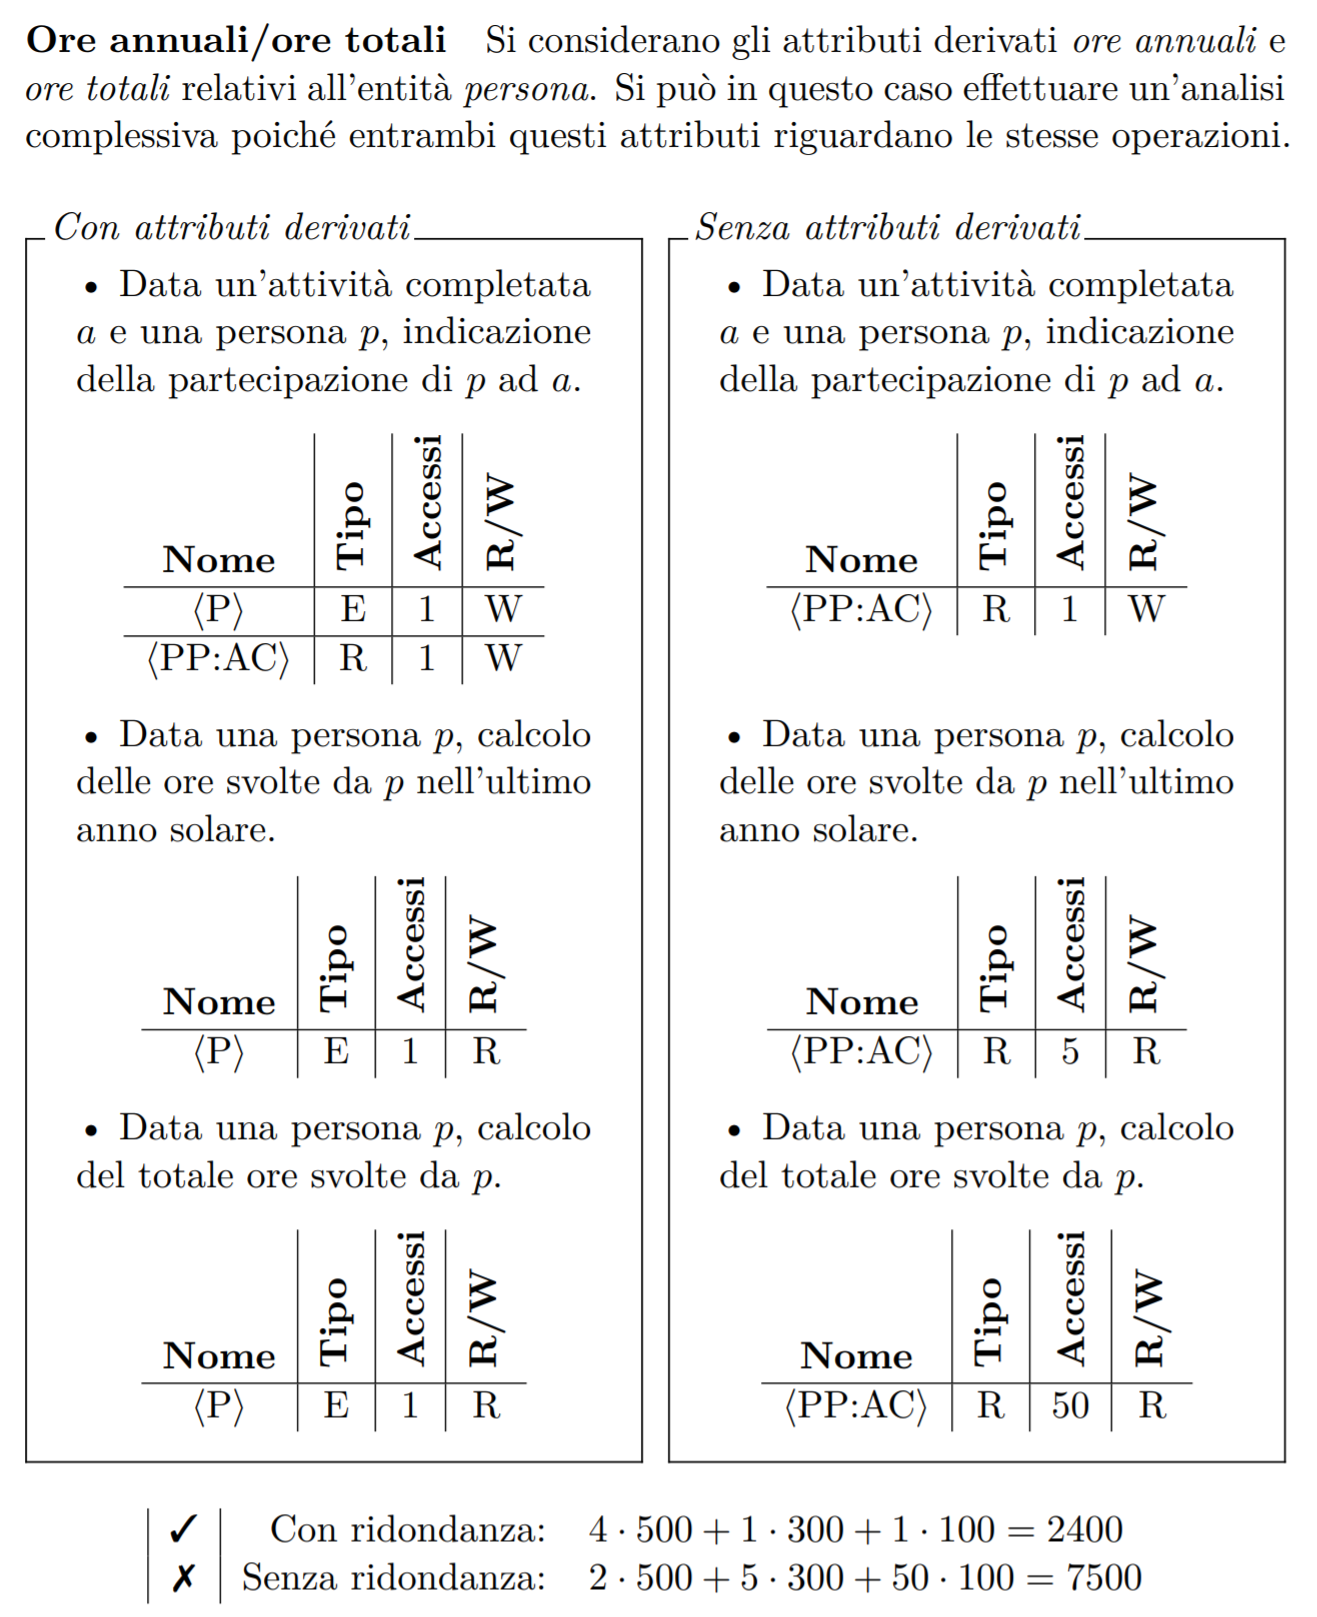
\includegraphics[width=0.6\textwidth]{img/tabella_accessi.png}
    \caption{Esempio di tabella degli accessi per l'analisi delle ridondanze}
\end{figure}

\paragraph{} Il risultato complessivo è lo \emph{schema ER ristrutturato}.

\begin{figure}[H]
    \centering
    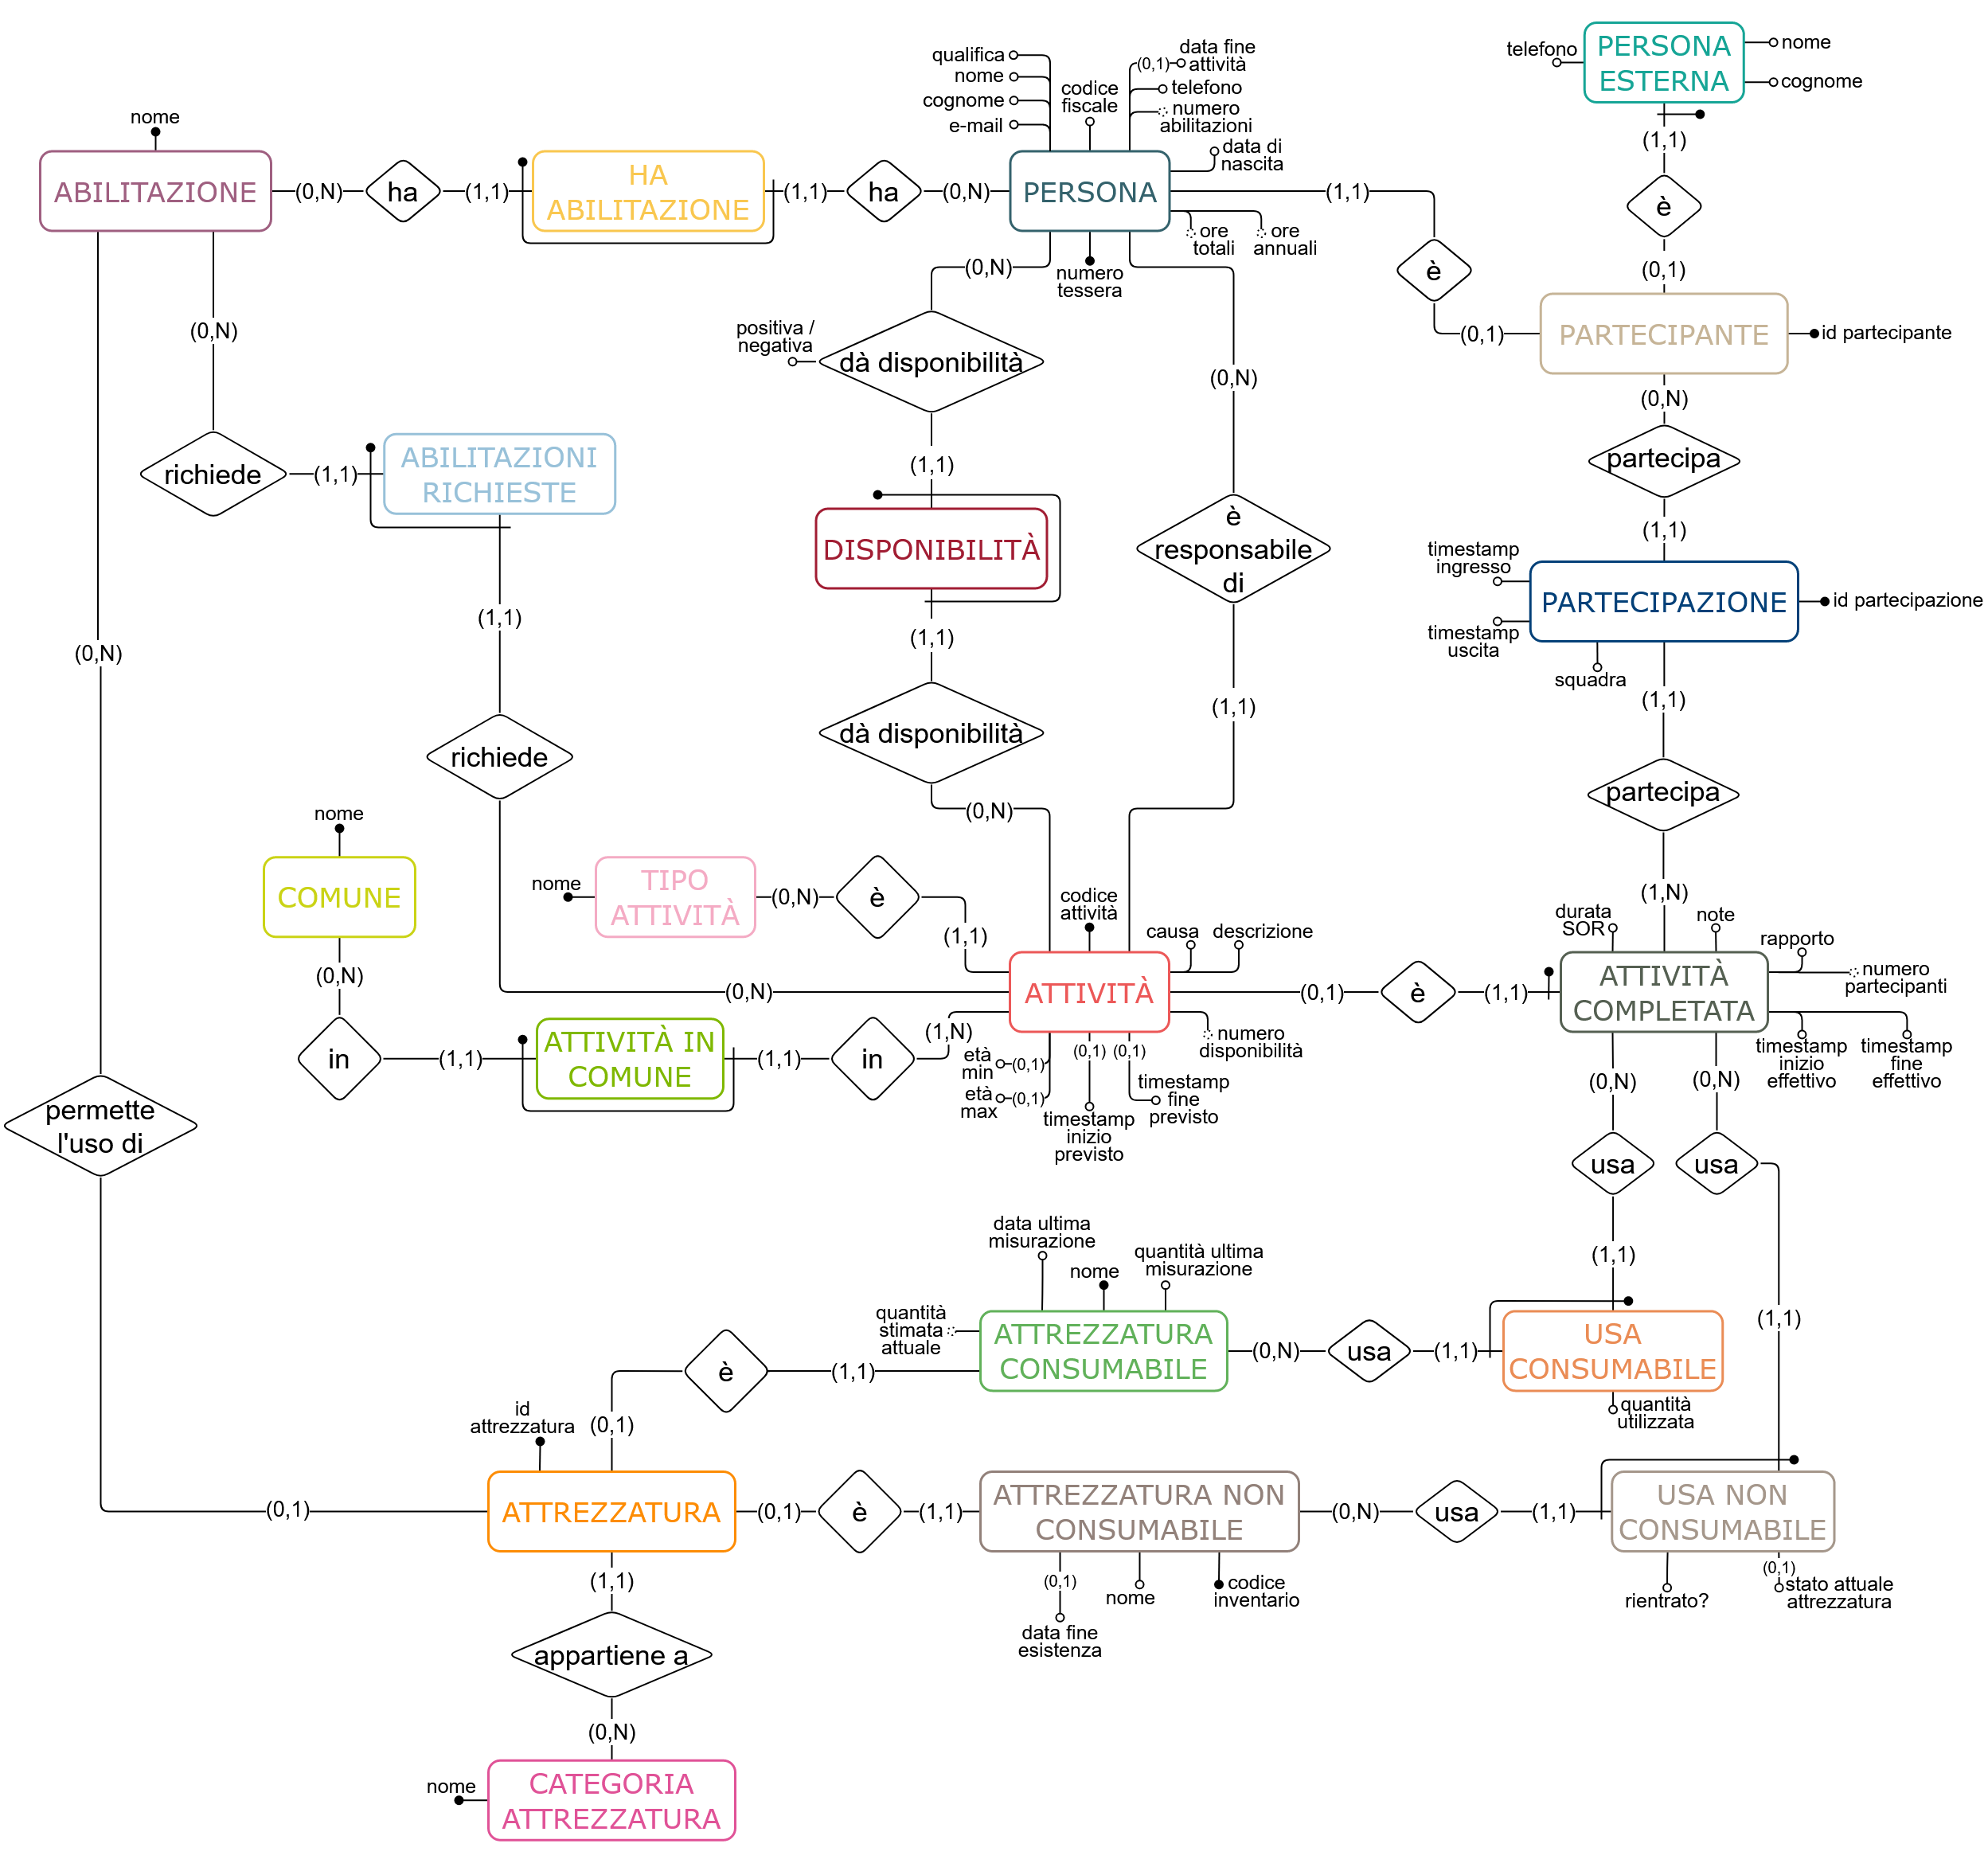
\includegraphics[width=0.8\textwidth]{img/er-ristrutturato.png}
    \caption{Schema ER ristrutturato}
\end{figure}

\subsection{Progettazione fisica e implementazione}

\paragraph{} Volendo sfruttare l'occasione del corso di laboratorio di Basi di Bati, a cui tutti i membri del gruppo di lavoro fanno parte, abbiamo deciso di procedere all'implementazione con il database relazionale \emph{PostgreSQL} \cite{postgre}. 

\paragraph{} L'implementazione delle entità e relazioni risulta naturale traducendo direttamente in SQL il contenuto dello schema ER ristrutturato. 

\begin{lstlisting}[language=SQL, caption=Esempio di implementazione di entità e relazioni]
CREATE TYPE qualifica_persona AS ENUM (
    'volontario', 'caposquadra', 'coordinatore'
);

CREATE TABLE persona (
    numero_tessera text PRIMARY KEY, -- Text = varchar(inf)
    id_partecipante int NOT NULL, -- Come chiave esterna, un serial diventa int | Il vincolo UNIQUE e' controllato dal trigger apposito
    codice_fiscale text NOT NULL UNIQUE, -- Era una chiave candidata
    nome text NOT NULL,
    cognome text NOT NULL,
    email text NOT NULL,
    telefono text NOT NULL,
    data_di_nascita date NOT NULL,
    data_fine_attivita date DEFAULT NULL,
    qualifica qualifica_persona NOT NULL,
    numero_abilitazioni int NOT NULL DEFAULT 0,
    ore_annuali interval NOT NULL DEFAULT interval '0 days',
    ore_totali interval NOT NULL DEFAULT interval '0 days',
    FOREIGN KEY (id_partecipante) REFERENCES partecipante(id_partecipante) ON DELETE NO ACTION ON UPDATE CASCADE
);

CREATE TABLE persona_esterna (
    id_partecipante int PRIMARY KEY, -- Il vincolo UNIQUE e' controllato dal trigger apposito
    nome text NOT NULL,
    cognome text NOT NULL,
    telefono text NOT NULL,
    FOREIGN KEY (id_partecipante) REFERENCES partecipante(id_partecipante) ON DELETE NO ACTION ON UPDATE CASCADE
);

CREATE TABLE ha_abilitazione (
    numero_tessera text,
    nome_abilitazione text,
    PRIMARY KEY (numero_tessera, nome_abilitazione),
    FOREIGN KEY (numero_tessera) REFERENCES persona(numero_tessera) ON DELETE CASCADE ON UPDATE CASCADE,
    FOREIGN KEY (nome_abilitazione) REFERENCES abilitazione(nome_abilitazione) ON DELETE CASCADE ON UPDATE CASCADE
);
\end{lstlisting}

\paragraph{} Sono stati definiti gli indici sui campi maggiormente utilizzati dalle query per la ricerca. 

\begin{lstlisting}[language=SQL, caption=Esempio di implementazione di indici]
CREATE INDEX idx_attivita_inizio ON attivita(timestamp_inizio_previsto, timestamp_fine_previsto);
CREATE INDEX idx_attivita_completata_inizio ON attivita_completata(timestamp_inizio_effettivo, timestamp_fine_effettivo); -- Per quantita' stimata di attrezzaura consumabile
CREATE INDEX idx_persona_partecipante ON persona(id_partecipante);
\end{lstlisting}

\paragraph{} Mediante la codifica di opportuni \emph{trigger}\footnote{I \emph{trigger} sono particolari script eseguibili all'interno di un dbms, a seguito della modifica dei suoi contenuti.} in linguaggio \emph{plpgsql}, abbiamo realizzato i principali controlli di integrità non verificabili dal dbms tramite i soli \emph{constraints}. Inoltre, trigger aggiuntivi sono stati aggiunti per facilitare l'inserimento di alcuni dati.

\begin{lstlisting}[language=SQL, caption=Esempio di implementazione di trigger]
-- Vincolo di esclusivita' attrezzatura (no duplicati) in inserimento
CREATE OR REPLACE FUNCTION check_id_attrezzatura()
RETURNS TRIGGER
LANGUAGE plpgsql AS $$
BEGIN
    IF EXISTS (
        (SELECT id_attrezzatura FROM attrezzatura_consumabile WHERE id_attrezzatura = new.id_attrezzatura)
        UNION
        (SELECT id_attrezzatura FROM attrezzatura_non_consumabile WHERE id_attrezzatura = new.id_attrezzatura)
    )
    THEN Raise Exception 'Duplicate id_attrezzatura: %', new.id_attrezzatura;
    END IF;
    RETURN new;
END;
$$;

DROP TRIGGER IF EXISTS trigger_02_insert_consumabile ON attrezzatura_consumabile; -- Il '02' nel nome serve perche' i trigger su una tabella sono controllati in ordine alfabetico
CREATE TRIGGER trigger_02_insert_consumabile
    BEFORE INSERT ON attrezzatura_consumabile
    FOR EACH ROW
    EXECUTE PROCEDURE check_id_attrezzatura();

DROP TRIGGER IF EXISTS trigger_insert_non_consumabile ON attrezzatura_non_consumabile;
CREATE TRIGGER trigger_insert_non_consumabile
    BEFORE INSERT ON attrezzatura_non_consumabile
    FOR EACH ROW
    EXECUTE PROCEDURE check_id_attrezzatura();
\end{lstlisting}


\subsection{Deploy locale}

\paragraph{} Per effettuare il testing preliminare, è stato effettuato il deploy di un'istanza locale tramite docker. 

\paragraph{} L'immagine scelta è \emph{postgres}, a cui basta passare le credenziali di amministrazione tramite environment. 

\begin{lstlisting}[caption=Configurazione di docker compose per postgres]
postgres:
    container_name: protezionecivile_pg
    image: postgres
    environment:
      POSTGRES_USER: postgres
      POSTGRES_PASSWORD: postgres
      PGDATA: /data/postgres
    volumes:
      - pgdata:/data/postgres
      - ./database:/base
    ports:
      - '5432:5432'
\end{lstlisting}


\subsubsection{Approfondimento: Utilizzo di Docker}

\paragraph{} \emph{Docker} \cite{docker} è una piattaforma software che permette di creare, testare e distribuire applicazioni in modo semplice e sicuro.\footnote{https://aws.amazon.com/it/docker/} 

\paragraph{} Esso raccoglie il software in unità standardizzate chiamate \emph{container}, le quali offrono tutto il necessario per la loro corretta esecuzione, incluse librerie, strumenti di sistema, codice e runtime. 

\paragraph{} Lavorando in un ambiente virtualizzato, si ha a disposizione un intero sistema operativo comprensivo di memoria stabile e risorse hardware (scheda di rete, gpu, ecc...), senza però rischiare di compromettere il proprio dispositivo. Infatti, se qualcosa dovesse andare storto, basta eliminare il containter difettoso ed avviarne uno nuovo!

\paragraph{} Il funzionamento è standardizzato: lo stesso container può essere eseguito senza sforzo in qualunque macchina che abbia installato Docker server. Un servizio testato in ambiente locale molto probabilmente funzionerà senza problemi una volta caricato nell'ambiente di produzione. Per questo, docker è particolarmente indicato per l'utilizzo nel cloud. 

\paragraph{} Docker è anche molto utile per gestire la scalabilità: con semplici comandi è possibile lanciare nuove istanze per affrontare immediatamente rapidi picchi di carico o fornire ridondanza. 

\paragraph{} \emph{Docker compose} è un'estensione di Docker che permette di specificare, mediante un file di configurazione unico in formato yaml, un insieme di istanze che lavorano in modo sinergico. In questo modo, è possibile usare un comando unico per effettuare il deploy di tutto il necessario per il progetto.

\begin{figure}[H]
    \centering
    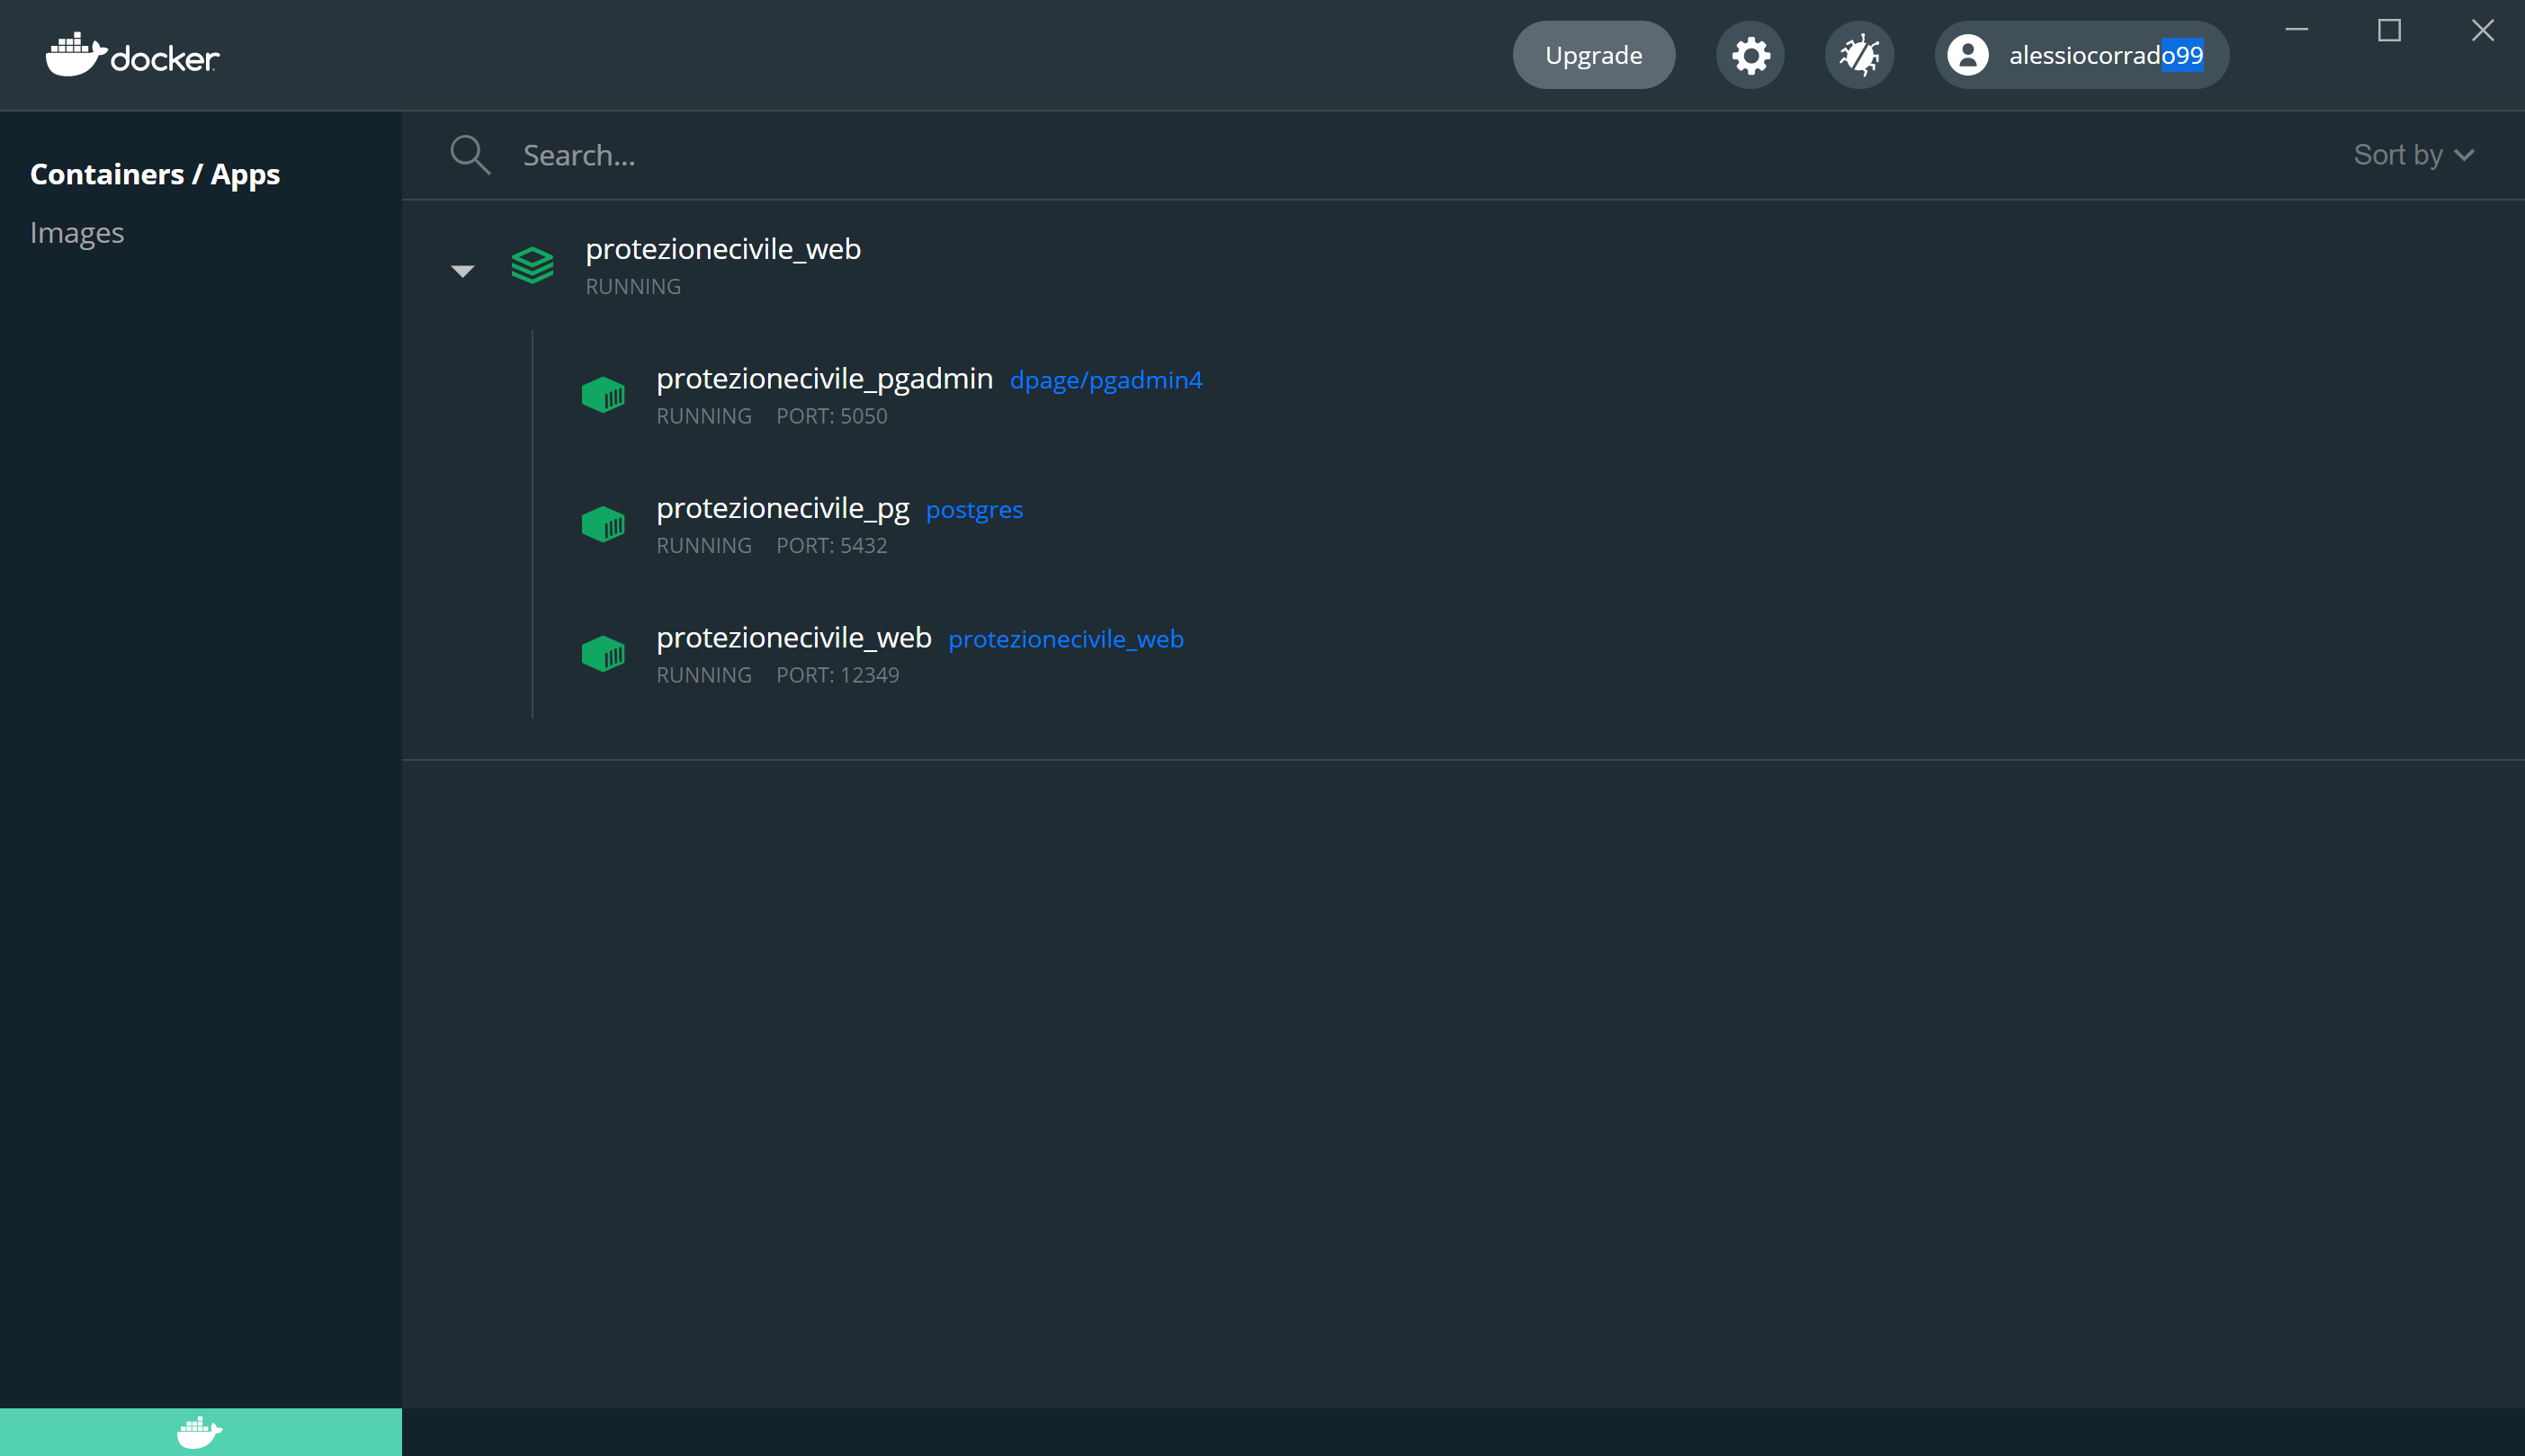
\includegraphics[width=0.8\textwidth]{img/docker.png}
    \caption{Utilizzo di Docker Desktop con i container usati nel progetto}
\end{figure}


\subsection{Testing}

\paragraph{} Per interfacciarsi con il postgres, si è scelto di usare la GUI \emph{pgAdmin4} \cite{pgadmin}.

\paragraph{} Un primo testing è stato effettuato inserendo manualmente query in modo da popolare il database con pochi dati, effettuare ricerche e modificarne il contenuto. Per ogni vincolo di integrità, è stata eseguita almeno una query che andasse a verificare il comportamento. 

\paragraph{} Successivamente, tramite l'utilizzo della libreria \emph{Faker} per linguaggio PHP, abbiamo popolato il database con dati realistici e conformi con la tabella dei volumi.

\begin{figure}[H]
    \centering
    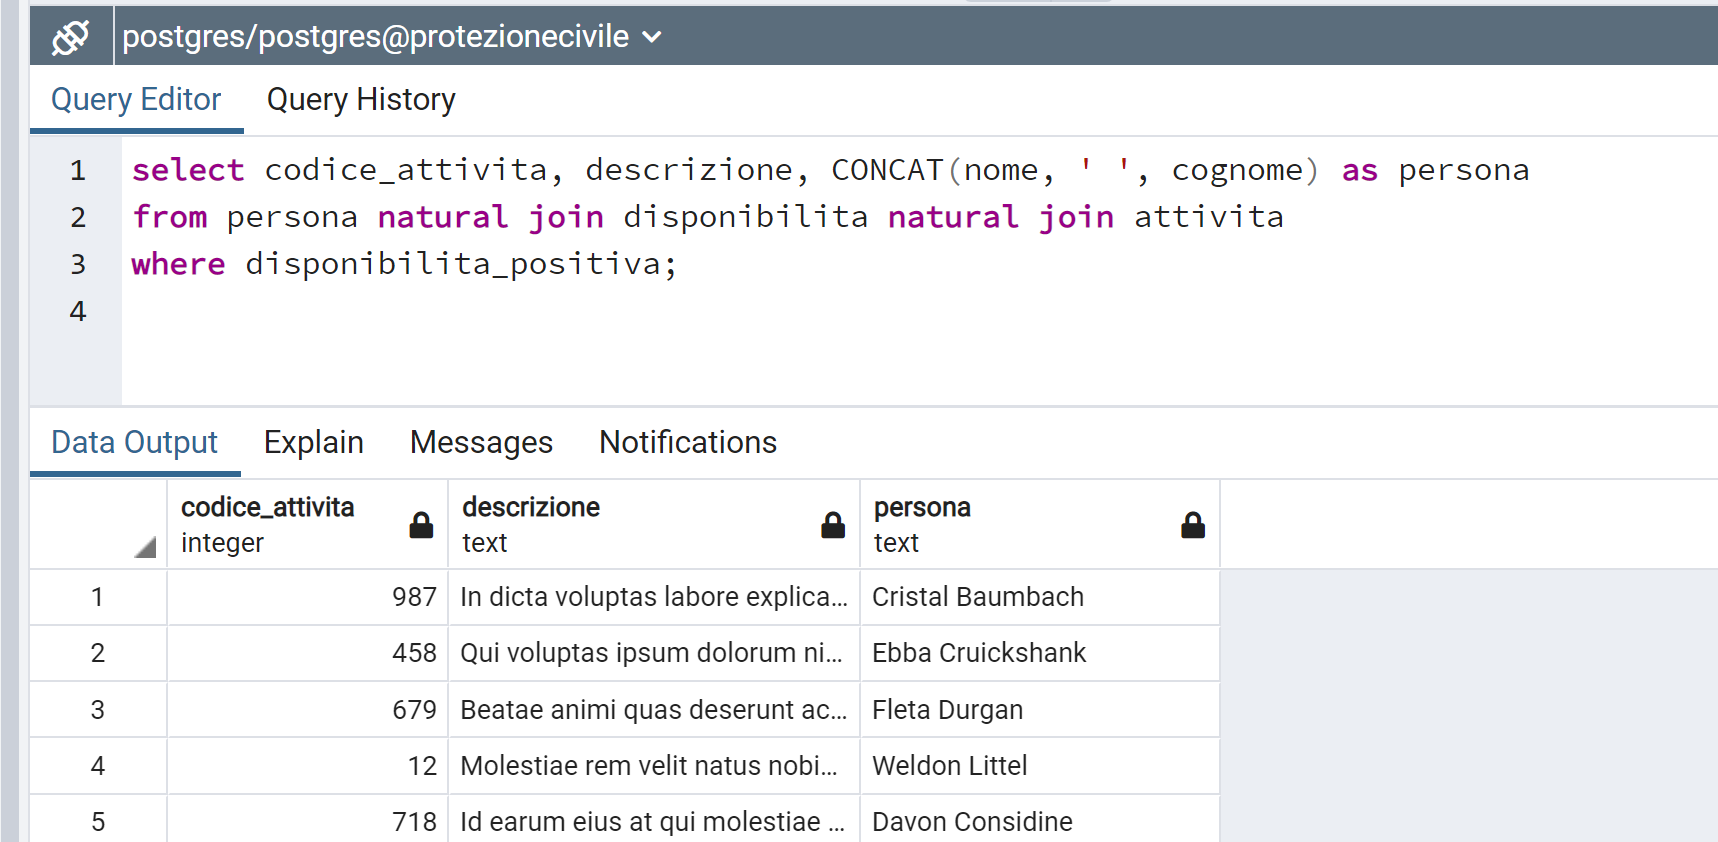
\includegraphics[width=0.8\textwidth]{img/query_esempio.png}
    \caption{Attività di testing sul database con pgAdmin4}
\end{figure}



\section{API web}

\paragraph{} Una volta concluso lo sviluppo del database, è stato affrontata la progettazione e sviluppo dell'API web \cite{restapi}.

\subsection{Progettazione}

\paragraph{} Per lo sviluppo di questa parte è stato scelto un approccio di tipo incrementale. Il primo incremento contiene solamente il minimo indispensabile per eseguire un server. Ad ogni incremento successivo, vengono aggiunti e testati nuovi endpoint.

\paragraph{} Per avere una migliore modularizzazione del codice, viene inizialmente costruita una libreria di supporto. Essa permette di effettuare in modo agevole le operazioni più comuni, come l'accesso al database e la formattazione della risposta. 

\paragraph{} La cache, implementata con \emph{Redis} \cite{redis}, permette di velocizzare le operazioni di recupero dei dati in lettura. Infatti, con essa non è necessario che il database e il server API ricalcolino la risposta ad ogni chiamata, ma possono inviare direttamente la risposta, se presente in cache.

\paragraph{} Per l'implementazione, si è scelto di usare il linguaggio \emph{Python 3} \cite{python} tramite framework \emph{Flask} \cite{flask}. Esso dispone nativamente di un server di sviluppo.  

\subsubsection{Approfondimento: Utilizzo di git per lo sviluppo incrementale}

\paragraph{} I sistemi di \emph{version control} sono sistemi specializzati nella gestione dei cambiamenti dei file. Uno dei sistemi di version control maggiormente utilizzati nell'ambito della produzione e manutenzione di software è il \emph{Git} \cite{git}.

\paragraph{} Il contenuto di un file in un certo istante viene chiamato \emph{versione}. Ad ogni versione è associato un \emph{timestamp}, e opzionalmente un identificativo. L'identificativo spesso è composto da un nome o da un codice. 

\paragraph{} Solitamente, si parte con un progetto vuoto. Alla creazione di ciascun documento, si ha la creazione della sua \emph{versione iniziale}. Ogni volta che si modifica un documento, ne viene creata una nuova versione, che va a sostituire la precedente. 

\paragraph{} Al raggiungimento di una \emph{milestone}, risoluzione di un bug, implementazione di una feature o qualsiasi altro punto di avanzamento dei lavori ritenuto "di interesse", tutte le ultime versioni dei documenti interessati vengono contrassegnate con un messaggio. Questa procedura si chiama \emph{commit}.

\begin{figure}[H]
    \centering
    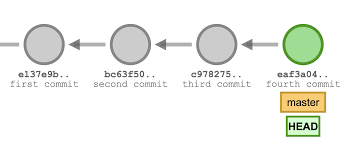
\includegraphics[width=0.7\textwidth]{img/git-history.png}
    \caption{Esempio di sequenza di commit, ciascuno con il proprio identificativo}
\end{figure}

\paragraph{} Nel caso in cui qualcosa dovesse andare storto, le operazioni di \emph{reset} e \emph{checkout} permettono di ripristinare la situazione a subito dopo uno qualsiasi dei commit precedenti. Il messaggio associato a ciascun commit permette di identificare facilmente il punto corretto da cui riprendere i lavori. 

\paragraph{} Nel caso si stia lavorando ad un estensione, oppure si voglia lavorare contemporaneamente a più incrementi, la strategia ottimale consiste nel creare \emph{branch multipli}. Il branch \emph{master} contiene la sequenza di commit del "programma principale". In qualsiasi momento, è possibile creare un nuovo branch e su di esso proseguire con il lavoro. 

\paragraph{} L'operazione di \emph{merge}, solitamente effettuata tra il \emph{branch di lavoro} e \emph{master}, permette di riunire i due branch, fondendoli. Il merge può consistere in una sovrascrittura di un branch sull'altro, oppure in una fusione in cui si tengono alcuni dati di un branch e alcuni dell'altro (nel caso in cui siano stati effettuati commit su entrambi i branch dopo la divisione). 


\begin{figure}[H]
    \centering
    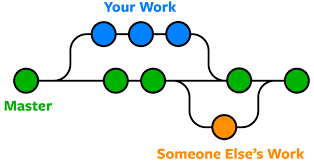
\includegraphics[width=0.6\textwidth]{img/git-condiviso.png}
    \caption{Esempio dell'uso di git in un progetto condiviso}
\end{figure}

\paragraph{} Le operazioni di \emph{push} e \emph{pull} permettono di sincronizzare il contenuto di un'istanza locale di git con un server condiviso. Ciò risulta fondamentale nel momento in cui si lavora in team, permettendo ad ogni membro di lavorare sui suoi branch e poi caricarli o fonderli assieme in uno spazio comune.


\begin{figure}[H]
    \centering
    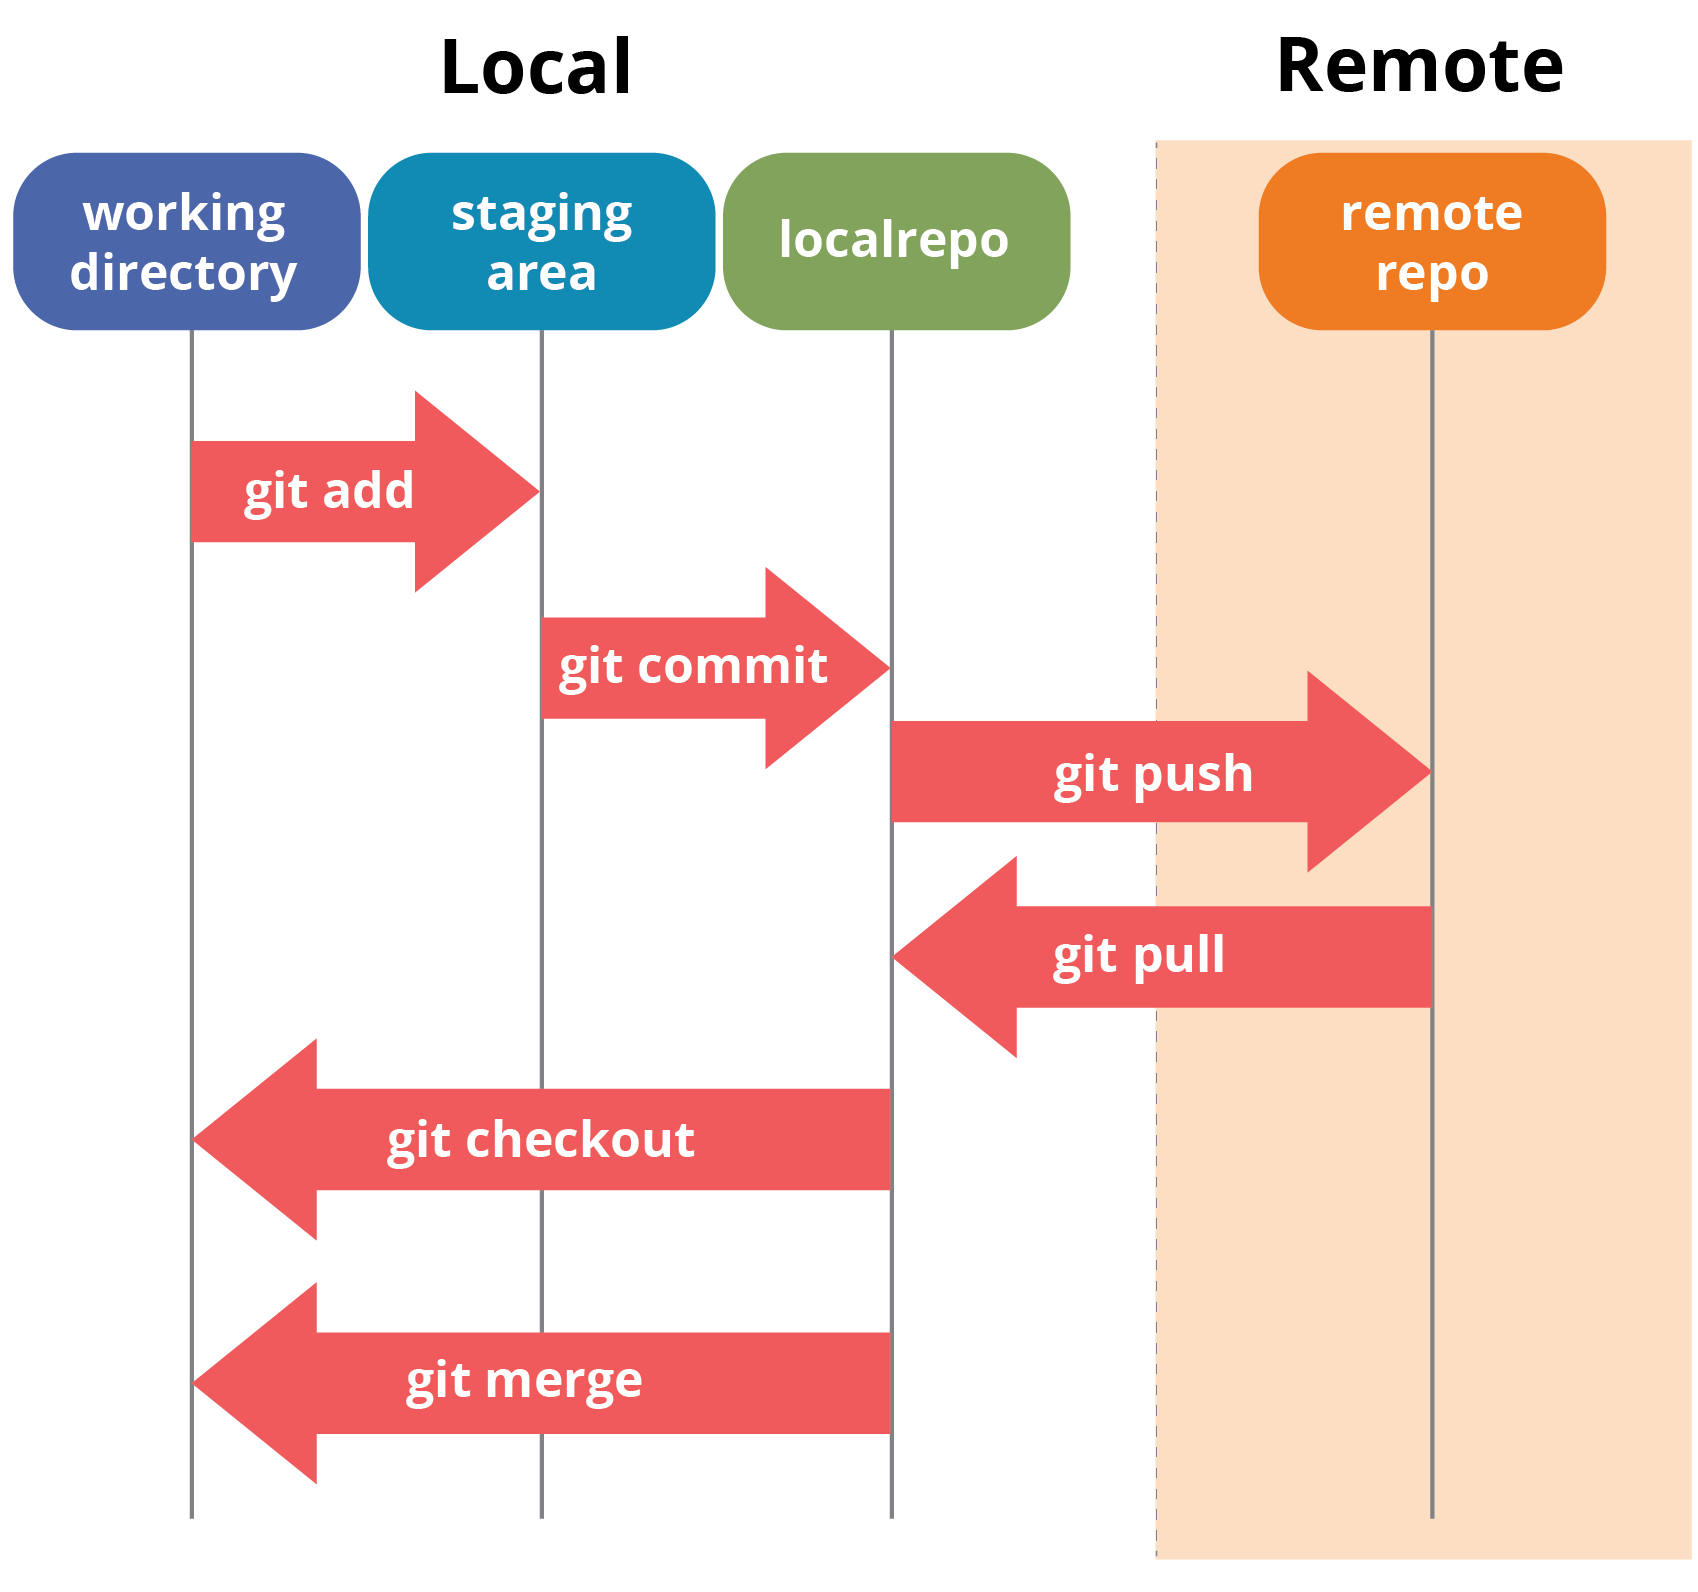
\includegraphics[width=0.8\textwidth]{img/git-ops.png}
    \caption{Operazioni principali durante l'utilizzo di git}
\end{figure}


\paragraph{} L'utilizzo di git si sposa con la metodologia dello \emph{sviluppo incrementale}. Infatti, è naturale associare ad ogni incremento un commit. Inoltre, l'utilizzo di branch separati permette di sviluppare in parallelo incrementi diversi senza che essi interferiscano fra loro, e permette di tenere separata la versione di \emph{produzione} da quella di \emph{sviluppo}.

\subsubsection{Approfondimento: WSGI}

\paragraph{} La \emph{Web Server Gateway Interface (WSGI)} \cite{wsgi} è una calling convention seguita dai server web per inoltrare le richieste ad applicazioni web o framework scritti in Python. 

\paragraph{} In precedenza, i webserver si interfacciavano con le webapp utilizzando una grande varietà di protocolli, a volte persino sviluppati ad hoc. L'adozione dell'interfaccia comune WSGI promuove la scrittura di codice portabile, riutilizzabile e standardizzato.

\paragraph{} WSGI ha due lati:
\begin{itemize}
    \item \emph{server/gateway}: un webserver completo, come \emph{nginx} o \emph{apache}, oppure una lightweight app che comunica con un server;
    \item \emph{application/framework}: un eseguibile scritto in Python che viene richiamato per gestire le richieste.
\end{itemize}

\paragraph{} I \emph{middleware} sono componenti inseriti tra server e application, che quindi implementano entrambi i lati di WSGI. Essi possono elaborare le richieste e/o inoltrarle ad altre applicazioni WSGI. Un utilizzo comune dei middleware è per inserire layer di log, autenticazione o gestione degli errori. 

\paragraph{} Un'applicazione compatibile con wsgi è composta da particolari funzioni generatrici, che accettano due parametri, \emph{environ} e \emph{start\_response}, e ritornano un flusso di byte (la risposta). Di seguito è riportato un esempio.

\begin{lstlisting}[language=python, caption=Applicazione hello world]
#application: il nome della funzione
#environ: un dizionario contenente le variabili d'ambiente CGI, i parametri della richiesta e altri parametri user-defined
#start_response: una funzione che accetta i parametri (status, response_headers)
def application(environ, start_response):
    start_response('200 OK', [('Content-Type', 'text/plain')])
    yield b'Hello, World!\n'
\end{lstlisting}

\paragraph{} Di seguito invece un'implementazione dimostrativa lato chiamante. 

\begin{lstlisting}[language=python, caption=Implementazione dimostrativa chiamante]
from io import BytesIO

def call_application(app, environ):
    status = None
    headers = None
    body = BytesIO()
    
    def start_response(rstatus, rheaders):
        nonlocal status, headers
        status, headers = rstatus, rheaders
        
    app_iter = app(environ, start_response)
    try:
        for data in app_iter:
            assert status is not None and headers is not None, \
                "start_response() was not called"
            body.write(data)
    finally:
        if hasattr(app_iter, 'close'):
            app_iter.close()
    return status, headers, body.getvalue()

environ = {...} 
status, headers, body = call_application(app, environ)
\end{lstlisting}

\paragraph{} Il framework Flask implementa lo standard WSGI. La sua facilità di utilizzo, unita all'elevata versatilità e alla compattezza del codice, lo rende particolarmente adatto allo sviluppo web.

\begin{lstlisting}[language=python, caption=Hello world con Flask]
app = Flask(__name__)

@app.route('/')
def hello():
    return "Hello World!"
\end{lstlisting}

\subsection{Inizializzazione del contesto}

\paragraph{} Inanzitutto è stato scritto il codice relativo all'inizializzazione di Flask e alla connessione con database e cache.

\begin{lstlisting}[language=python, caption=Inizializzazione del server]
app = Flask(__name__, template_folder="template")

if __name__ == '__main__':
    app.run(host='0.0.0.0', port=8080, debug=True)
\end{lstlisting}

\begin{lstlisting}[language=python, caption=Connessione al database]
db_config = {
    'user': os.environ.get('SQL_USERNAME'),
    'password': os.environ.get('SQL_PASSWORD'),
    'database': os.environ.get('SQL_DATABASE_NAME'),
    'host': os.environ.get('SQL_HOST')
}
cnxpool = psycopg2.pool.ThreadedConnectionPool(minconn=1, maxconn=100, **db_config)
\end{lstlisting}

\begin{lstlisting}[language=python, caption=Connessione alla cache Redis]
redis_host = os.environ.get('REDISHOST')
redis_port = os.environ.get('REDISPORT')

redis_client = redis.StrictRedis(host=redis_host, port=int(redis_port)) if redis_host is not None else None
\end{lstlisting}


\subsection{Costruzione libreria di supporto}

\paragraph{} La libreria di supporto è stata costruita in modo da supportare al meglio lo sviluppo di questo progetto. Essendo però generica, potrà essere facilmente utilizzata dagli sviluppatori per eventuali progetti futuri.

\paragraph{} La funzione \emph{do} è quella di più basso livello. Essa inanzitutto apre una connessione al database (\emph{cnx}). Viene poi applicata la funzione \emph{query}, contenente la logica della chiamata. Essa restituisce un risultato sotto forma di oggetto, il quale viene formattato per l'invio tramite \emph{applyRes}.  

\begin{lstlisting}[language=python, caption=Funzione \emph{do}]
def defaultToJson(data):
    return json.dumps(data, indent=4, sort_keys=True, default=str)


def do(query, applyRes = defaultToJson):
    cnx = cnxpool.getconn()
    with cnx.cursor(cursor_factory=psycopg2.extras.RealDictCursor) as cursor:
        res = query(cursor)

    res = applyRes(res)
    cnx.commit()
    cnxpool.putconn(cnx)

    return res
\end{lstlisting}

\paragraph{} Le funzioni \emph{cursor\_*} astraggono le operazioni più comuni sul database, fornendo un'interfaccia per effettuare le query standard di \emph{insert}, \emph{update} e \emph{delete} su singola tabella. \emph{select} non è inclusa in quanto utilizzare una funzione generica è più difficoltoso che scrivere direttamente la query in linguaggio SQL. 

\begin{lstlisting}[language=python, caption=Funzioni \emph{cursor\_*}]
#data: dict contenente i dati da inserire/modificare
#table: nome tabella
#fields: lista degli attributi della tabella
#cond: lista degli attributi che compongono la chiave primaria
#returning: stringa contenente il nome da associare alla clausola returning (per la generazione di valori da parte del database)

def cursor_insert(cursor, data, table, fields, returning=None):
    #inserisci solo valori effettivamente presenti in data
    #cio' permette di inserire solo alcune colonne, e lasciare il valore di default nelle rimanenti
    fields = list(filter(lambda x: x in data.keys(), fields))

    #generazione dinamica della query
    #'%s' viene usato come placeholder per iniettare i valori in modo safe (contro attacchi di tipo sql injection)
    s1 = ", ".join(fields)
    s2 = ", ".join(map(lambda x: "%s", fields))

    query = "insert into " + table + "(" + s1 + ") values (" + s2 + ") "

    if returning is not None:
        query += " returning " + returning

    #binding tra placeholder e valori effettivi
    vals = [data[i] for i in fields]

    #esecuzione della query nel db
    cursor.execute(query, vals)


def cursor_update(cursor, data, table, fields, cond, returning=None):
    fields = list(filter(lambda x: x in data, fields))

    s1 = ", ".join(map(lambda x: x + "=%s", fields))
    s2 = ", ".join(map(lambda x: x + "=%s", cond))

    query = "update " + table + " set " + s1 + " where " + s2
    if returning is not None:
        query += " returning " + returning

    vals = [data[i] for i in fields + cond]

    cursor.execute(query, vals)

def cursor_delete(cursor, data, table, cond):
    s2 = " and ".join(map(lambda x: x + "=%s", cond))

    query = "delete from " + table + " where " + s2

    vals = [data[i] for i in cond]

    cursor.execute(query, vals)
\end{lstlisting}

\paragraph{} Le funzioni \emph{generate\_*} creano gli endpoint associati a metodi standard, per effettuare le operazioni corrispondenti su singola tabella. 

\paragraph{} Gli endpoint sono standardizzati. Ad esempio, il metodo per effettuare un update dell'entità \emph{persona} viene generato all'endpoint \emph{POST /api/update\_persona}. 

\begin{lstlisting}[language=python, caption=Funzioni \emph{generate\_*}]
#table, fields, cond, returning hanno lo stesso significato delle funzioni cursor_*
#prefix: il prefisso delle chiamate API

def generate_create(table, fields, returning, prefix="/api"):
    def f_create():
        #contenuto del body della richiesta, parsing da formato json
        data = request.json

        def f(cursor):
            #inserimento nel database tramite interfaccia cursor_*
            cursor_insert(cursor, data, table, fields, returning)

            #default per risposta con successo
            res = {"message": "ok"}

            #includi nella risposta quanto generato dalla clausola returning
            if returning:  
                v = cursor.fetchone()
                res[returning] = v[returning]

            return res

        return do(f)

    #creazione dinamica dell'endpoint associato alla richiesta
    app.add_url_rule(prefix + "/create_" + table, "create_" + table, f_create, methods=["POST"])
    

def generate_update(table, fields, cond, returning, prefix="/api"):
    def f_update():
        data = request.json

        def f(cursor):
            cursor_update(cursor, data, table, fields, cond, returning)

            ... come insert...

        return do(f)

    app.add_url_rule(prefix + "/update_" + table, "update_" + table, f_update, methods=["POST"])


def generate_set(table, fields, prefix="/api"):
    def f_set():
        data = request.json

        def f(cursor):
            #elimina tutte le righe nel database
            cursor.execute("delete from " + table)

            #inserisce in modo batch ogni riga in input
            for elem in data:
                cursor_insert(cursor, elem, table, fields)

            return {"message": "ok"}

        return do(f)

    app.add_url_rule(prefix + "/set_" + table, "set_" + table, f_set, methods=["POST"])


def generate_delete(table, cond, prefix="/api"):
    def f_delete():
        data = request.json

        def f(cursor):
            cursor_delete(cursor, data, table, cond)

            return {"message": "ok"}

        return do(f)

    app.add_url_rule(prefix + "/delete_" + table, "delete_" + table, f_delete, methods=["DELETE"])


def generate_get(table, query=None, prefix="/api"):
    #la query di default seleziona tutte le colonne e tutte le righe della tabella
    if query is None:
        query = "select * from " + table

    def f_get():
        data = request.json

        def f(cursor):
            cursor.execute(query)

            #nel caso la query ritorni una sola riga, e' comunque contenuta in una lista unitaria [row1]
            #lista vuota [] nel caso in cui la query non ritorni alcuna riga
            return cursor.fetchall()

        return do(f)

    app.add_url_rule(prefix + "/get_" + table, "get_" + table, f_get, methods=["GET"])
\end{lstlisting}

\paragraph{} La funzione \emph{generate\_crsd} genera gli endpoint per effettuare le operazioni \emph{create}, \emph{read}, \emph{update} e \emph{delete} su una singola entità.

\begin{lstlisting}[language=python, caption=generate\_crsd]
def generate_crsd(table, fields, cond=None, returning=None, prefix="/api"):
    if cond is None:
        cond = fields

    generate_create(table, fields, returning, prefix=prefix)
    generate_delete(table, cond, prefix=prefix)
    generate_get(table, prefix=prefix)
    generate_set(table, fields, prefix=prefix)
\end{lstlisting}

\subsection{Implementazione API}

\paragraph{} Una volta completata la libreria di supporto, è possibile implementare la logica dell'applicazione. 

\paragraph{} Di seguito, tutte le chiamate di cui si possono generare automaticamente gli endpoint.

\begin{lstlisting}[language=python, caption=Endpoint generati automaticamente]
generate_crsd("categoria_attrezzatura", ["nome_categoria"])
generate_crsd("tipo_attivita", ["nome_tipo_attivita"])
generate_crsd("comune", ["nome_comune"])
generate_crsd("abilitazione", ["nome_abilitazione"])
generate_crsd("ha_abilitazione", ["nome_abilitazione", "numero_tessera"])
generate_crsd("abilitazioni_richieste", ["codice_attivita", "nome_abilitazione"])
generate_crsd("attivita_in_comune", ["codice_attivita", "nome_comune"])
generate_crsd("usa_consumabile", ["codice_attivita", "nome_attrezzatura", "quantita_utilizzata"],
              ["codice_attivita", "nome_attrezzatura"])
generate_crsd("usa_non_consumabile", ["codice_attivita", "codice_inventario", "rientrato", "stato_attuale_attrezzatura"],
              ["codice_attivita", "codice_inventario"])
generate_crsd("partecipazione", ["id_partecipante", "codice_attivita", "squadra", "timestamp_ingresso", "timestamp_uscita"],
              ["codice_attivita", "id_partecipante"])
generate_crsd("persona_esterna", ["nome", "cognome", "telefono"], ["id_partecipante"], returning="idPartecipante")
generate_crsd("disponibilita", ["codice_attivita", "numero_tessera", "disponibilita_positiva"],
              ["codice_attivita", "numero_tessera"])


generate_delete("attivita", ["codice_attivita"])
generate_delete("attivita_completata", ["codice_attivita"])
generate_delete("persona", ["numero_tessera"])
generate_delete("attrezzatura", ["id_attrezzatura"])


generate_get("persona")
generate_get("attrezzatura_consumabile", query="SELECT * from attrezzatura natural join attrezzatura_consumabile")
generate_get("attrezzatura_non_consumabile", query="SELECT * from attrezzatura natural join attrezzatura_non_consumabile")
\end{lstlisting}

\paragraph{} Per concludere, sono presenti tutti gli endpoint complessi, non generabili automaticamente. Si noti come vengano comunque sfruttate le funzioni di libreria.

\begin{lstlisting}[language=python, caption=Esempio di endpoint non generabile]
@app.route('/api/get_persona_dettagli', methods=["GET"])
def get_persona_dettagli():
    #parametri in ingresso
    numero_tessera = request.args.get("numero_tessera")
    if numero_tessera is None:
        return defaultToJson({"errore": "numero_tessera null"}), 400

    def f(cursor):  #codice che utilizza il database
        cursor.execute(
            'SELECT * from persona '
            'where numero_tessera = %s', (numero_tessera, ))

        res = cursor.fetchone()

        if res is None:
            return None

        cursor.execute("select nome_abilitazione from ha_abilitazione where numero_tessera = %s", (numero_tessera, ))
        res["ha_abilitazione"] = cursor.fetchall()

        cursor.execute("select * from disponibilita "
                       "natural join attivita "
                       "where numero_tessera = %s", (numero_tessera,))
        res["disponibilita"] = cursor.fetchall()

        cursor.execute("select * from persona "
                       "natural join partecipazione "
                       "natural join attivita_completata natural join attivita "
                       "where numero_tessera = %s", (numero_tessera,))
        res["partecipazione"] = cursor.fetchall()


        return res

    return do(f)
\end{lstlisting}

\subsection{Autenticazione}

\paragraph{} L'autenticazione dell'utente avviene tramite credenziali \cite{password}. Per poter essere riconosciuto dal sistema, l'utente deve fornire una coppia \emph{username, password} valida. 

\paragraph{} Per avere un discreto livello di sicurezza, è bene richiedere l'utilizzo di password prive di significato, con lunghezza congrua (almeno 8-10 caratteri) e non utilizzate altrove. 

\paragraph{} Ad ogni profilo utente è associato un livello di autorizzazione. I livelli di autorizzazione sono\begin{itemize}
    \item \emph{login}: l'utente ha un profilo. Default per la visualizzazione dei dati;
    \item \emph{crea\_evento}: l'utente può creare, modificare ed eliminare eventi. Utilizzato da coloro che si occupano dell'inserimento dati; 
    \item \emph{cms}: può effettuare attività di content management (ad esempio modificare l'elenco dei comuni o creare una nuova persona). 
\end{itemize}

\paragraph{} L'accesso ad endpoint API protetti avviene tramite \emph{access token}. L'utente può ottenere un nuovo access token tramite una richiesta di \emph{login}, alla quale fornisce username e password. La richiesta di \emph{logout} elimina permanentemente l'access token. 

\paragraph{} Password, access token e autorizzazioni sono conservati in due tabelle dedicate nel database: \emph{auth} per password e autorizzazioni, \emph{token} per gli access token. 

\begin{lstlisting}[language=SQL, caption=tabelle auth e token]
create table auth(
    email text primary key,
    password text not null,
    numero_tessera text,
    crea_evento boolean not null,
    cms boolean not null,
    foreign key (numero_tessera) references persona(numero_tessera) on update cascade on delete cascade
);

create table token(
    token text primary key,
    email text not null,
    foreign key (email) references auth(email) on update cascade on delete cascade
);

-- default admin 
insert into auth(email, password, numero_tessera, crea_evento, cms) values ('admin', 'admin', null, True, True);
\end{lstlisting}

\paragraph{} L'endpoint \emph{do\_login} si occupa di effettuare il login.

\paragraph{} Email e password sono ricercati nella tabella \emph{auth}. Se non ci sono corrispondenze, la chiamata ritorna errore \emph{401 Unauthorized}. Se invece viene trovata una corrispondenza (che per forza è univoca, essendo \emph{email} chiave univoca), si procede alla generazione del token.

\paragraph{} Il token è composto dal numero tessera concatenato ad una stringa casuale di lunghezza 32. Il numero tessera prefisso permette di identificare il proprietario del token. La stringa casuale viene scelta in modo da avere solo caratteri inseribili in un URL, per evitare di doverla ricodificare nella risposta. 

\paragraph{} Una volta generato il token, lo si inserisce nella tabella \emph{token} associandolo all'email dell'utente (chiave primaria di \emph{auth}). 

\paragraph{} Il token viene incluso nel corpo della risposta, in modo da poter essere utilizzato dal client. 

\begin{lstlisting}[language=Python, caption=POST do\_login]
@app.route("/api/do_login", methods=["POST"])
def doLogin():
    data = getDataSettingNull()

    def f(cursor):
        cursor.execute("select * from auth where email=%s and password=%s", (data["email"], data["password"]))
        row = cursor.fetchone()

        if row is None:
            return {"message": "not found", "token": None}, 401

        row["token"] = str(row["numero_tessera"]) + secrets.token_urlsafe(32)

        cursor_insert(cursor, row, "token", ["token", "email"])

        return {"message": "ok", "token": row["token"]}

    return do(f, auth=None)
\end{lstlisting}

\begin{figure}[H]
    \centering
    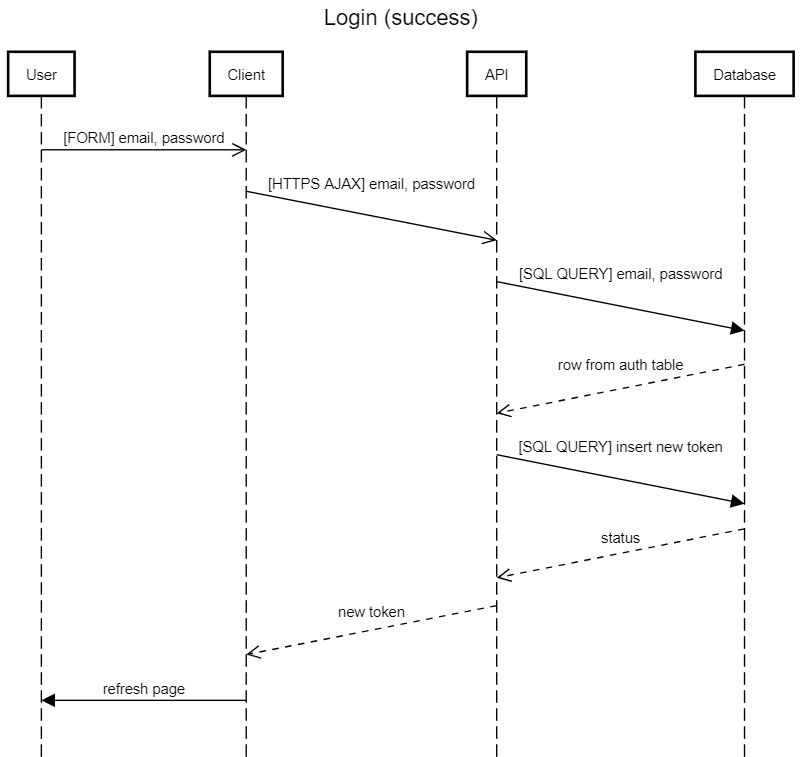
\includegraphics[width=0.8\textwidth]{img/Login (success).png}
    \caption{Creazione di un nuovo access token (successo)}
\end{figure}

\paragraph{} Per associare la propria identità ad una richiesta, il client scrive il valore del proprio token nel campo \emph{Authorization} della richiesta HTTPs. 

\paragraph{} La funzione ausiliaria \emph{getLogin} si occupa di ottenere i dati e le autorizzazioni dell'utente che ha effettuato una richiesta. Per far ciò, legge il token dall'header Authorization e lo ricerca nel database.


\begin{lstlisting}[language=Python, caption=funzione ausiliaria getLogin]
def getLogin(cursor):
    token = request.headers.get("Authorization")

    cursor.execute("select * from token natural join auth where token=%s", (token, ))
    row = cursor.fetchone()

    if row is not None:
        del row["password"]  #nascondi la password per maggiore sicurezza
 
    return row
\end{lstlisting}

\paragraph{} La funzione di supporto \emph{do} è stata modificata per includere il controllo di autorizzazione. 

\paragraph{} Essa, prima di effettuare la query, controlla che il livello di autorizzazione dell'utente sia adeguato. Se il parametro \emph{auth} è una stringa, identifica il nome del livello di autorizzazione. Se esso è None, il controllo delle autorizzazioni è disabilitato. Se auth è una funzione, viene interpretato come una funzione booleana che, date le autorizzazioni e i dati dell'utente, restituisce \emph{True} se l'utente è autorizzato. 

\emph{} Nel caso in cui l'utente non disponga delle autorizzazioni necessarie, viene inviata una risposta contenente un codice d'errore adeguato (401 se il token non è valido, 403 se non dispone di sufficienti autorizzazioni).

\begin{lstlisting}[language=Python, caption=Funzione ausiliaria do modificata]
def do(query, applyRes = defaultToJson, auth="cms"):
    cnx = cnxpool.getconn()
    with cnx.cursor(cursor_factory=psycopg2.extras.RealDictCursor) as cursor:
        if auth is not None:
            permissions = getLogin(cursor)
            if permissions is not None: permissions["login"] = True

            if isinstance(auth, str):
                if permissions is None:
                    return applyRes({"message": "E' necessario effettuare il login"}, 401)
                if not permissions[auth]:
                    return applyRes({"message": "E' necessaria un'autorizzazione di tipo " + auth}, 403)
            else:
                auth(cursor, permissions)

        res = query(cursor)

    res = applyRes(res)
    cnx.commit()
    cnxpool.putconn(cnx)

    return res
\end{lstlisting}

\paragraph{} Le funzioni di supporto per la generazione automatica di endpoint sono state modificate in modo da includere l'autorizzazione richiesta. 

\begin{lstlisting}[language=Python, caption=Esempio di funzione generatrice di endpoint modificata e relativa chiamata]
def generate_create(table, fields, returning, auth="cms", prefix="/api"):
    def f_create():
        ...

        def f(cursor):
           ...

        return do(f, auth=auth)

    ...
    
    
def generate_crsd(table, fields, cond=None, returning=None, auth="cms", auth_get="login", prefix="/api"):
    if auth_get == "same":
        auth_get = auth

    if cond is None:
        cond = fields

    generate_create(table, fields, returning, auth=auth, prefix=prefix)
    generate_delete(table, cond, auth=auth, prefix=prefix)
    generate_get(table, auth=auth_get, prefix=prefix)
    generate_set(table, fields, auth=auth, prefix=prefix)
    generate_update(table, fields, cond, returning, auth=auth, prefix=prefix)
    
    
generate_crsd("categoria_attrezzatura", ["nome_categoria"], auth="cms")
\end{lstlisting}

\begin{figure}[H]
    \centering
    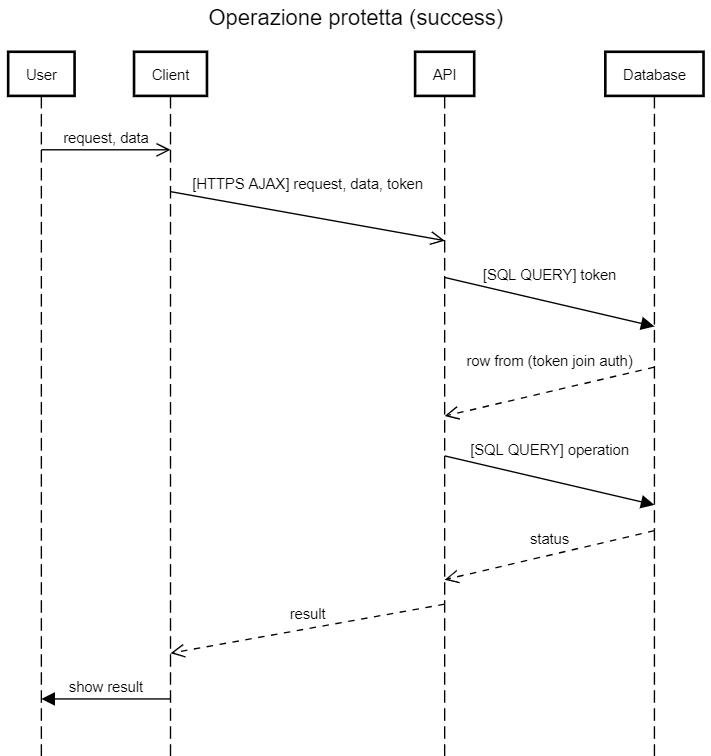
\includegraphics[width=0.8\textwidth]{img/Operazione protetta (success).png}
    \caption{Esecuzione di una richiesta protetta (successo)}
\end{figure}


\paragraph{} Il logout è effettuabile mediante l'endpoint \emph{do\_logout}. L'unico parametro richiesto è il token da eliminare. 

\begin{lstlisting}[language=Python, caption=POST do\_logout]
@app.route("/api/do_logout", methods=["POST"])
def doLogout():
    token = request.headers.get("Authorization")
    if token is None:
        return {"res": "token null"}, 400

    def f(cursor):
        cursor.execute("delete from token where token = %s returning token", (token, ))

        return {"message": "ok", "data": cursor.fetchone()}

    return do(f, auth=None)
\end{lstlisting}

\begin{figure}[H]
    \centering
    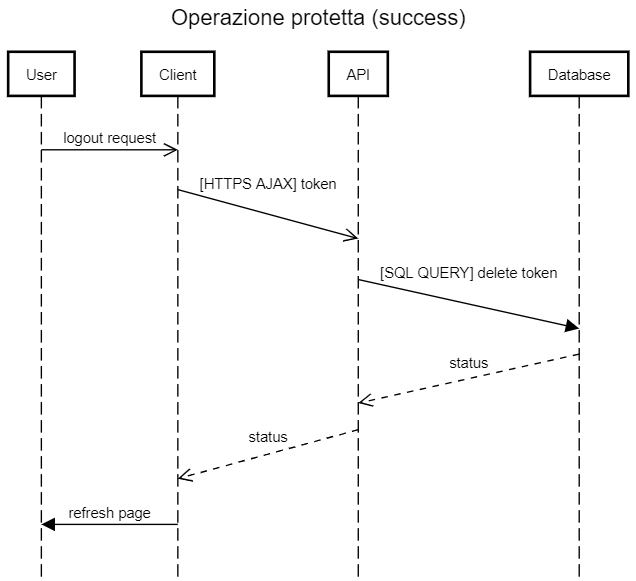
\includegraphics[width=0.8\textwidth]{img/Logout (success).png}
    \caption{Logout ed eliminazione token (successo)}
\end{figure}

\paragraph{} Il recupero della password è possibile solo tramite email. 

\paragraph{} Tramite richiesta all'endpoint \emph{richiedi\_recupera\_pw}, il sistema invia un'email all'indirizzo specificato contenente un link alla pagina \emph{recupera\_pw}.

\paragraph{} All'interno del link viene generato un token univoco, associato all'utente. Esso è a tutti gli effetti un access token legato alla email specificata, con cui il proprietario può modificare la password o effettuare altre operazioni.  

\begin{lstlisting}[language=Python, caption=endpoint richiedi\_recupera\_pw]
@app.route("/api/richiedi_recupera_pw", methods=["POST"])
def get_recuperaPw():
    data = getDataSettingNull()

    def f(cursor):
        d = dict()
        d["token"] = secrets.token_urlsafe(20)
        d["email"] = data["email"]

        cursor_insert(cursor, d, "token", ["token", "email"])
        
        ...

        me, you = "pc.cms.sanvito@gmail.com", d["email"]

        msg = MIMEMultipart('alternative')
        msg['Subject'] = "Link"
        msg['From'] = me
        msg['To'] = you

        link = "http://localhost:8080/render/recupera_pw?token=" + d["token"]

        text = "Segui il link per recuperare la password\n" + link
        html = """\
        <html>
          <head></head>
          <body>
            <p>Recupero password<br>
               Segui il link per recuperare la password<br>
               <a href=""" + link + """>link</a>
            </p>
          </body>
        </html>
        """

        ...

        server = smtplib.SMTP(smtp_server, port)
        server.starttls(context=context)  # Secure the connection
        server.login(sender_email, password)
        server.sendmail(me, you, msg.as_string())
        server.quit()

        return {"message": "ok"}

    return do(f, auth=None)
\end{lstlisting}


\begin{figure}[H]
    \centering
    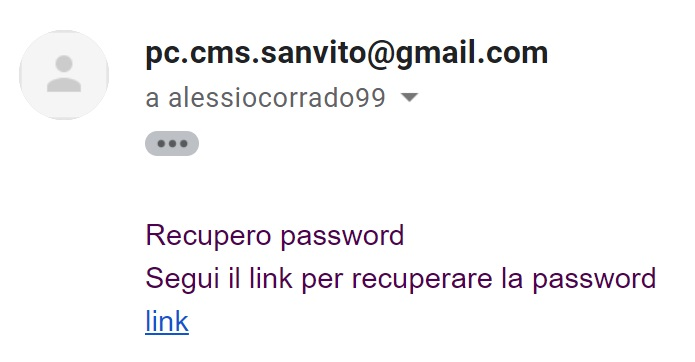
\includegraphics[width=0.6\textwidth]{img/email_recupero.jpg}
    \caption{Email di recupero password}
\end{figure}


\paragraph{} L'endpoint \emph{recupera\_pw} si occupa di impostare la nuova password per l'utente, se la richiesta è valida.

\paragraph{} Il recupero password elimina tutti i token associati all'utente. In questo modo, il recupero password permette di eliminare eventuali token rubati ed evitare che chi conosceva la vecchia password possa continuare ad operare. 

\begin{lstlisting}[language=Python, caption=POST recupera\_pw]
@app.route("/api/recupera_pw", methods=["POST"])
def do_recuperaPw():
    token = request.headers.get("Authorization")
    data = getDataSettingNull()

    def f(cursor):
        cursor.execute("select * from token natural join auth where email=%s and token=%s", (data["email"], token))
        row = cursor.fetchone()

        if row is None:
            return {"message": "not found"}, 401

        data["email_old"] = data["email"]
        cursor_update(cursor, data, "auth", ["password"], ["email"])
        cursor_delete(cursor, data, "token", ["email"])

        return {"message": "ok"}

    return do(f, auth=None)
\end{lstlisting}


\subsection{Testing}

\paragraph{} Il testing è immediato da eseguire: Flask mette a disposizione un suo server di test, richiamabile includendo all'interno dello script la funzione \emph{run}. La funzione di debug permette di leggere agevolmente i log e risalire ai punti in cui vengono lanciate delle eccezioni.

\paragraph{} Per poter interfacciarsi con il server è consigliabile utilizzare un \emph{client REST}. Quello scelto dallo sviluppatore è \emph{Insomnia} \cite{insomnia}.

\paragraph{} Nel caso specifico, il testing è stato eseguito provando a richiamare ogni endpoint e passando diverse combinazioni di dati, sia validi che non, verificando che i risultati fossero congrui alle specifiche.


\begin{figure}[H]
    \centering
    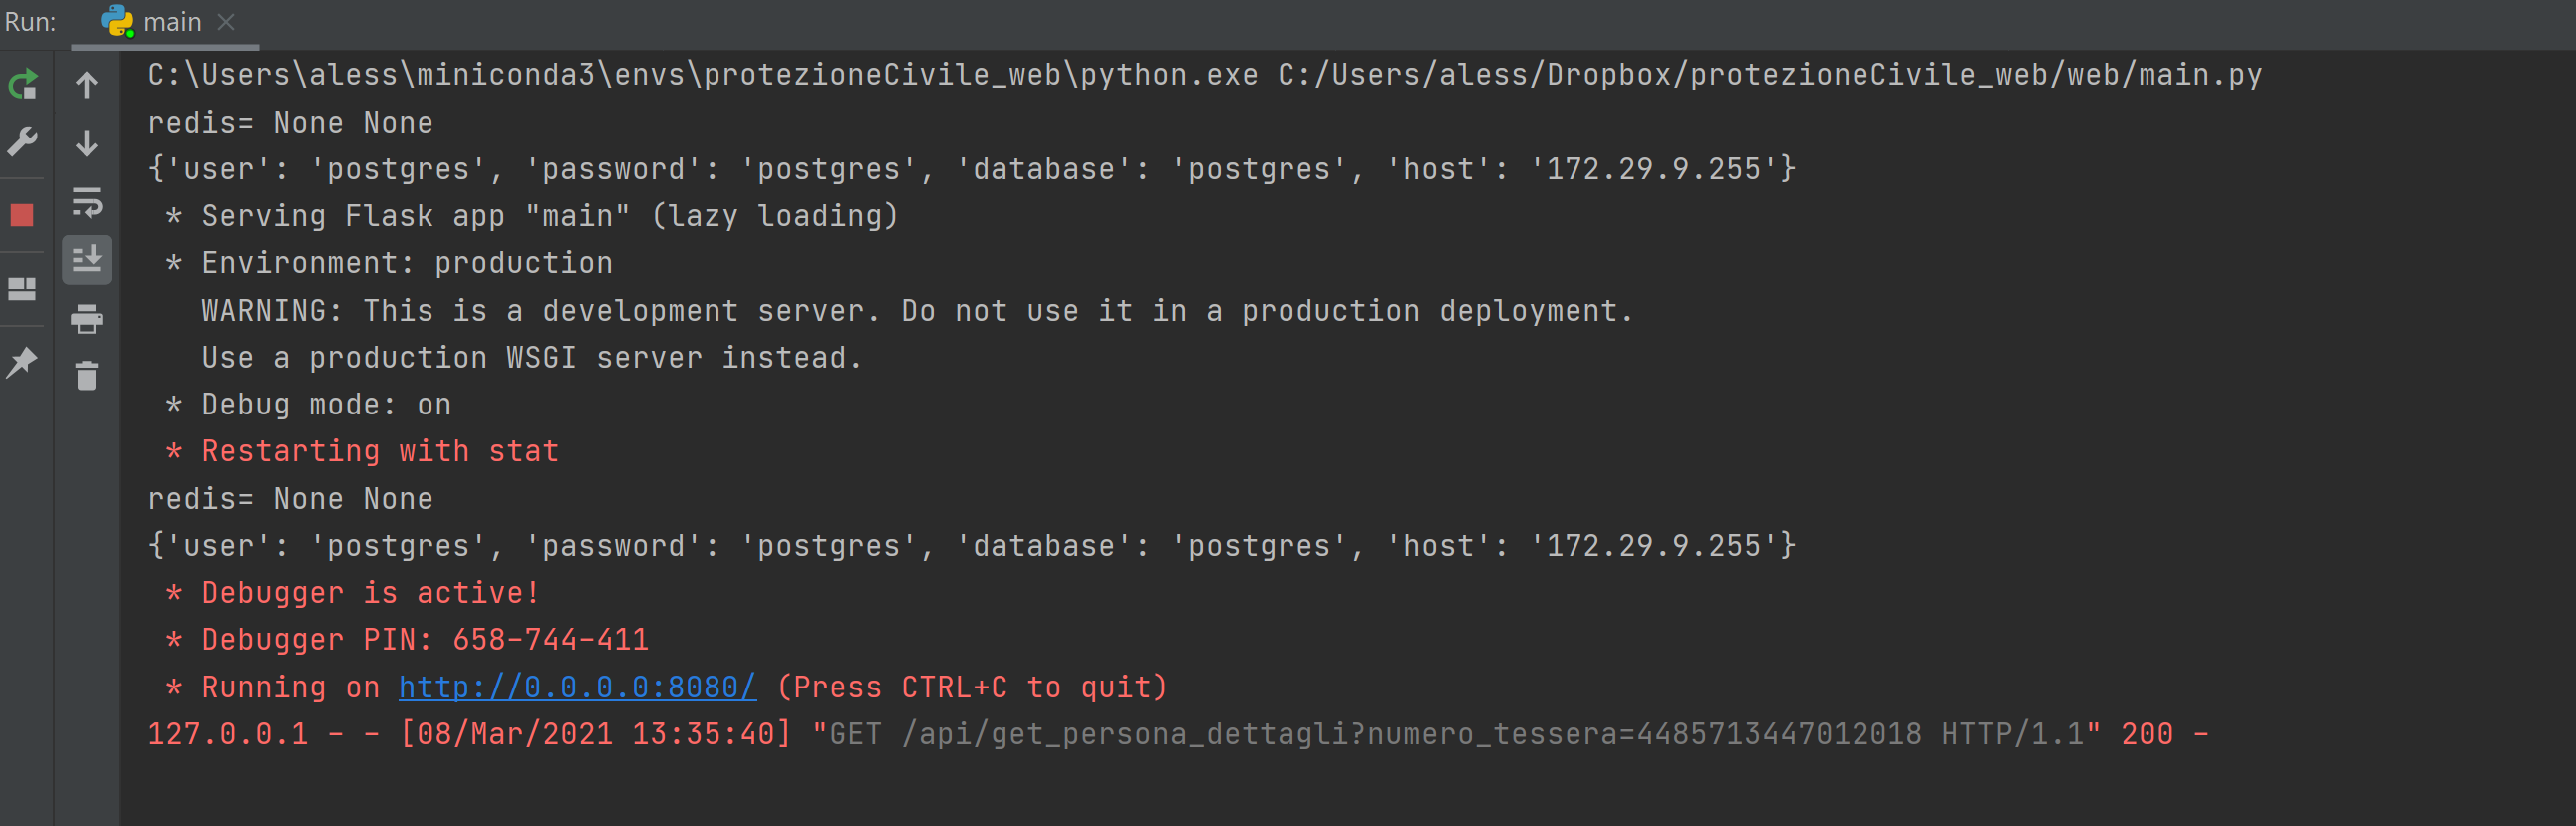
\includegraphics[width=0.8\textwidth]{img/api_debug.png}
    \caption{Console di debug per Flask}
\end{figure}


\begin{figure}[H]
    \centering
    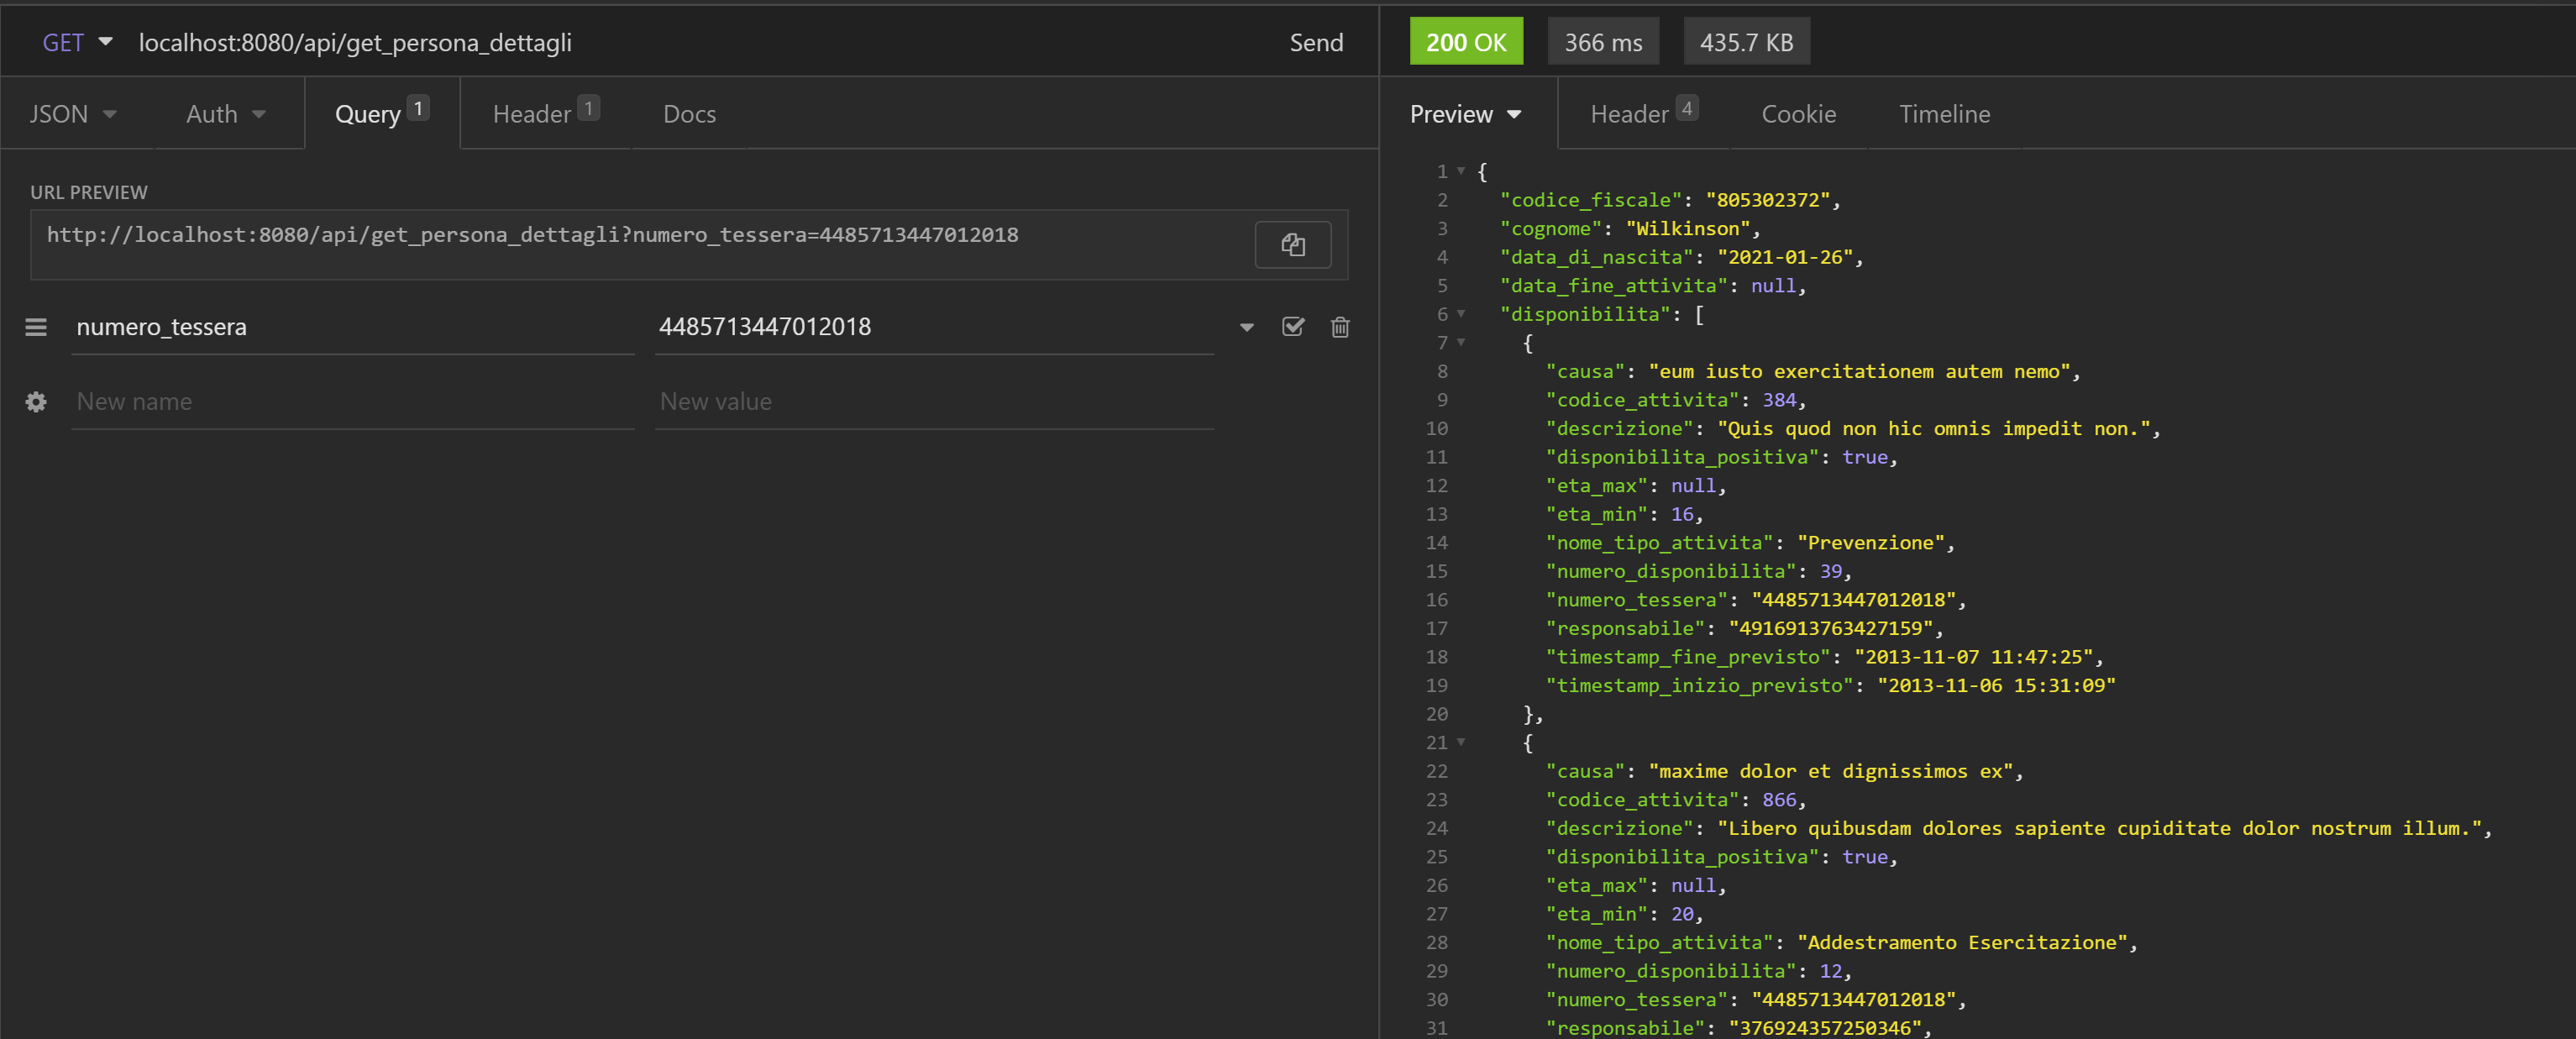
\includegraphics[width=0.8\textwidth]{img/insomnia.png}
    \caption{Utilizzo del client REST Insomnia}
\end{figure}



\subsection{Deploy locale}

\paragraph{} Il deploy è stato nuovamente effettuato creando un'istanza Docker. Come server di produzione è stato scelto di usate \emph{gunicorn}, uno dei più famosi per Flask.

\paragraph{} Per creare il container, è necessario partire da un'immagine contenente python3+gunicorn, installare le librerie necessarie e copiare i sorgenti.

\begin{lstlisting}[caption=Dockerfile]
FROM tiangolo/meinheld-gunicorn:python3.7
COPY requirements.txt /
RUN pip install -r /requirements.txt
COPY . /app
\end{lstlisting}

\begin{lstlisting}[caption=File di configurazione per Docker compose]
web:
    container_name: protezionecivile_web
    image: protezionecivile_web
    environment:
      SQL_USERNAME: postgres
      SQL_PASSWORD: postgres
      SQL_DATABASE_NAME: postgres
      SQL_HOST: 172.29.9.255
    volumes:
      - ./web:/app
    ports:
      - "<porta esterna>:80"
\end{lstlisting}



\section{Suddivisione dei compiti tra app e website}

\paragraph{} Applicazione e sito web sono complementari. Per questo sorge spontanea una domanda: per ogni funzionalità, dove metterla? 

\paragraph{} Dopo aver dialogato con il committente è risultato chiaro che la quasi totalità dei membri preferisce accedere ai contenuti tramite smartphone. Per questo motivo tutte le funzionalità "operative" vanno sicuramente incluse all'interno dell'app. 

\paragraph{} Per quanto riguarda invece la parte di \emph{content management}, lo schermo di maggiori dimensioni, unito alla possibilità di consultare in parallelo fogli excel e altri tipi di documento, suggeriscono che l'utilizzo da PC sia preferibile. Queste operazioni inoltre vengono svolte di rado (al massimo un paio di volte l'anno) e solamente da pochi membri designati come responsabili. 

\paragraph{} Quello che rimane è la consultazione dei grafici interattivi e statistiche varie. Risulta quindi opportuno inserire queste funzionalità sia nell'applicazione, magari in formato ridotto, sia nell'interfaccia web, con la possibilità di una maggiore possibilità di personalizzazione.






\section{App}

\paragraph{} Lo sviluppo dell'app è una delle parti più ostiche. Oltre alle difficoltà di programmazione, è importante anche andare incontro ai gusti degli utilizzatori, per fornire una buona estetica ed usabilità. 

\paragraph{} In questa sezione verrà affrontato l'intero processo di sviluppo dell'app, che quindi conterrà anche una parte meno "tecnica", ma altrettanto necessaria: il \emph{design} \cite{design}.

\subsection{Design} 

\paragraph{} Inanzitutto, è stato fissato un incontro con il committente incentrato sul design dell'applicazione. Sposando la filosofia "user-centered", è importante includere il più possibile l'utilizzatore finale, in particolare per quanto riguarda il design di interfaccia. 


\paragraph{} Inizialmente si sono identificate le azioni che l'utente svolge durante il lavoro. 

\begin{lstlisting}[title=Lista dei task]
Effettuare il login/logout
Fornire la disponibilita' per un'attivita'
Vedere i dettagli di un'attivita'
Vedere la lista delle attivita' future
Modificare una delle proprie disponibilita'
...

SOLO PER I COORDINATORI
Creare un'attivita'
Gestire le presenze di un'attivita' in svolgimento
Terminare e registrare un'attivita' in svolgimento
Gestire i materiali di un'attivia'
...
\end{lstlisting}

\paragraph{} Mediante la tecnica di \emph{task analysis}, le azioni sono state scomposte in \emph{passaggi} semplici. 

\begin{lstlisting}[title=Task analysis]
EFFETTUARE IL LOGIN
Se l'utente ha salvato le credenziali: 
    Effettua il login automaticamente e vai alla schermata principale
Altrimenti:
    Inserisci nome utente 
    Inserisci password
    Effettua login
    Se login corretto:
        Vai alla schermata principale
    Altrimenti: 
        Riprova
        
        
FORNIRE LA DISPONIBILITA' PER UN'ATTIVITA'
Visualizza la lista di attivita'
Scegli l'attivita' a cui dare la disponibilita'
Inserisci l'orario della disponibilita'
Conferma l'inserimento della disponibilita'


INSERIRE UNA PRESENZA PER UN'ATTIVITA' IN SVOLGIMENTO
Visualizza le attivita' in svolgimento
Scegli l'attivita' a cui aggiungere la presenza
Scegli la persona di cui inserire la presenza
Inserisci l'orario di arrivo 
Conferma l'inserimento della presenza


CREARE UN'ATTIVITA'
Inserisci il nome dell'attivita'
Scegli il tipo dell'attivita'
Inserisci la causa dell'attivita'
Inserisci la descrizione dell'attivita'
Inserisci la data di svolgimento dell'attivita'
Inserisci l'ora di inizio prevista dell'attivita'
Inserisci l'ora di fine prevista dell'attivita'
Se ci sono vincoli di eta':
    Inserisci l'eta' minima di partecipazione
    Inserisci l'eta' massima di partecipazione
Scegli i comuni in cui si svolgera' l'attivita'
Scegli le abilitazioni richieste per lo svolgimento dell'attivita'
Scegli il responsabile dell'attivita'
Conferma l'inserimento della nuova attivita' 

...
\end{lstlisting}

\paragraph{} Si noti la scelta dei verbi nella task analysis:
\begin{itemize}
    \item \textit{Scegli}: scelta da un insieme di elementi possibili;
    \item \textit{Inserisci}: inserimento da parte dell'utente;
    \item \textit{Effettua}: compimento di un'azione che non prevede scelte o inserimenti;
    \item \textit{Vai}: cambio di contesto;
    \item \textit{Conferma}: conferma esplicita al termine di una procedura.
\end{itemize}

\paragraph{} Le azioni sono state raggruppate in \emph{concetti}, organizzati in modo gerarchico. Il grafo dei concetti è la base per creare la struttura della \emph{navigazione}. 

\begin{figure}[H]
    \centering
    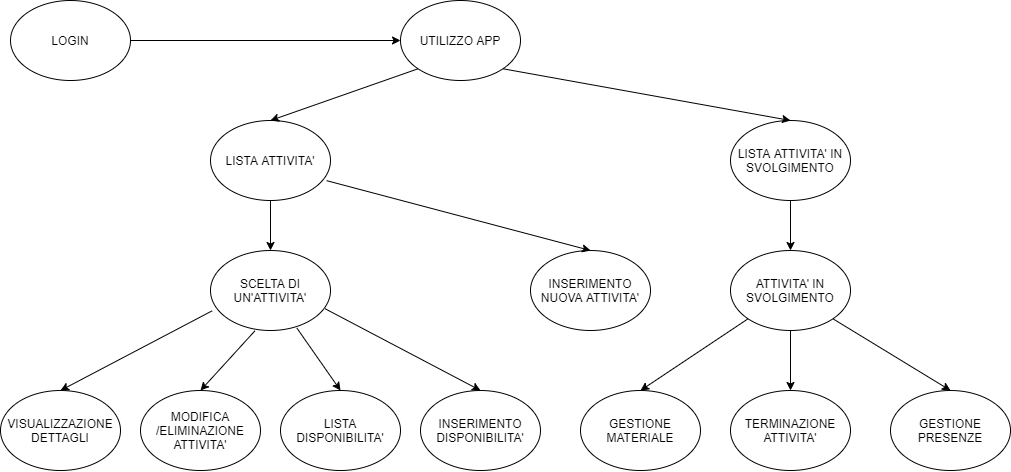
\includegraphics[width=0.8\textwidth]{img/concetti task app.png}
    \caption{Grafo dei concetti}
\end{figure}


\paragraph{} Come interfaccia di navigazione principale. è stato scelto di usare una sidebar. Il suo contenuto è il seguente: 
\begin{itemize}
    \item Nome e tipologia profilo
    \item Home
    \item Storico
    \item Statistiche
    \item Impostazioni
    \item Calendario
    \item Logout
\end{itemize}


\begin{figure}[H]
    \centering
    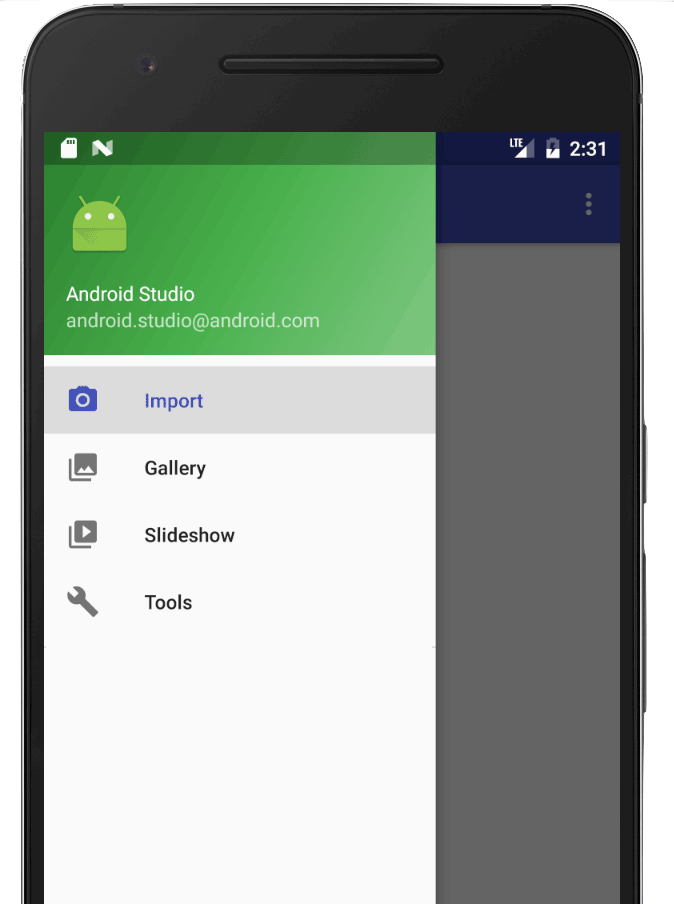
\includegraphics[width=0.3\textwidth]{img/sidebar-example.png}
    \caption{Esempio di sidebar}
\end{figure}

\paragraph{} Sono stati quindi creati i wireframe: rappresentazioni grafiche delle schermate dell'app, collegate tramite frecce. All'interno dei wireframe ci sono anche brevi descrizioni dei componenti grafici.

\begin{figure}[H]
    \centering
    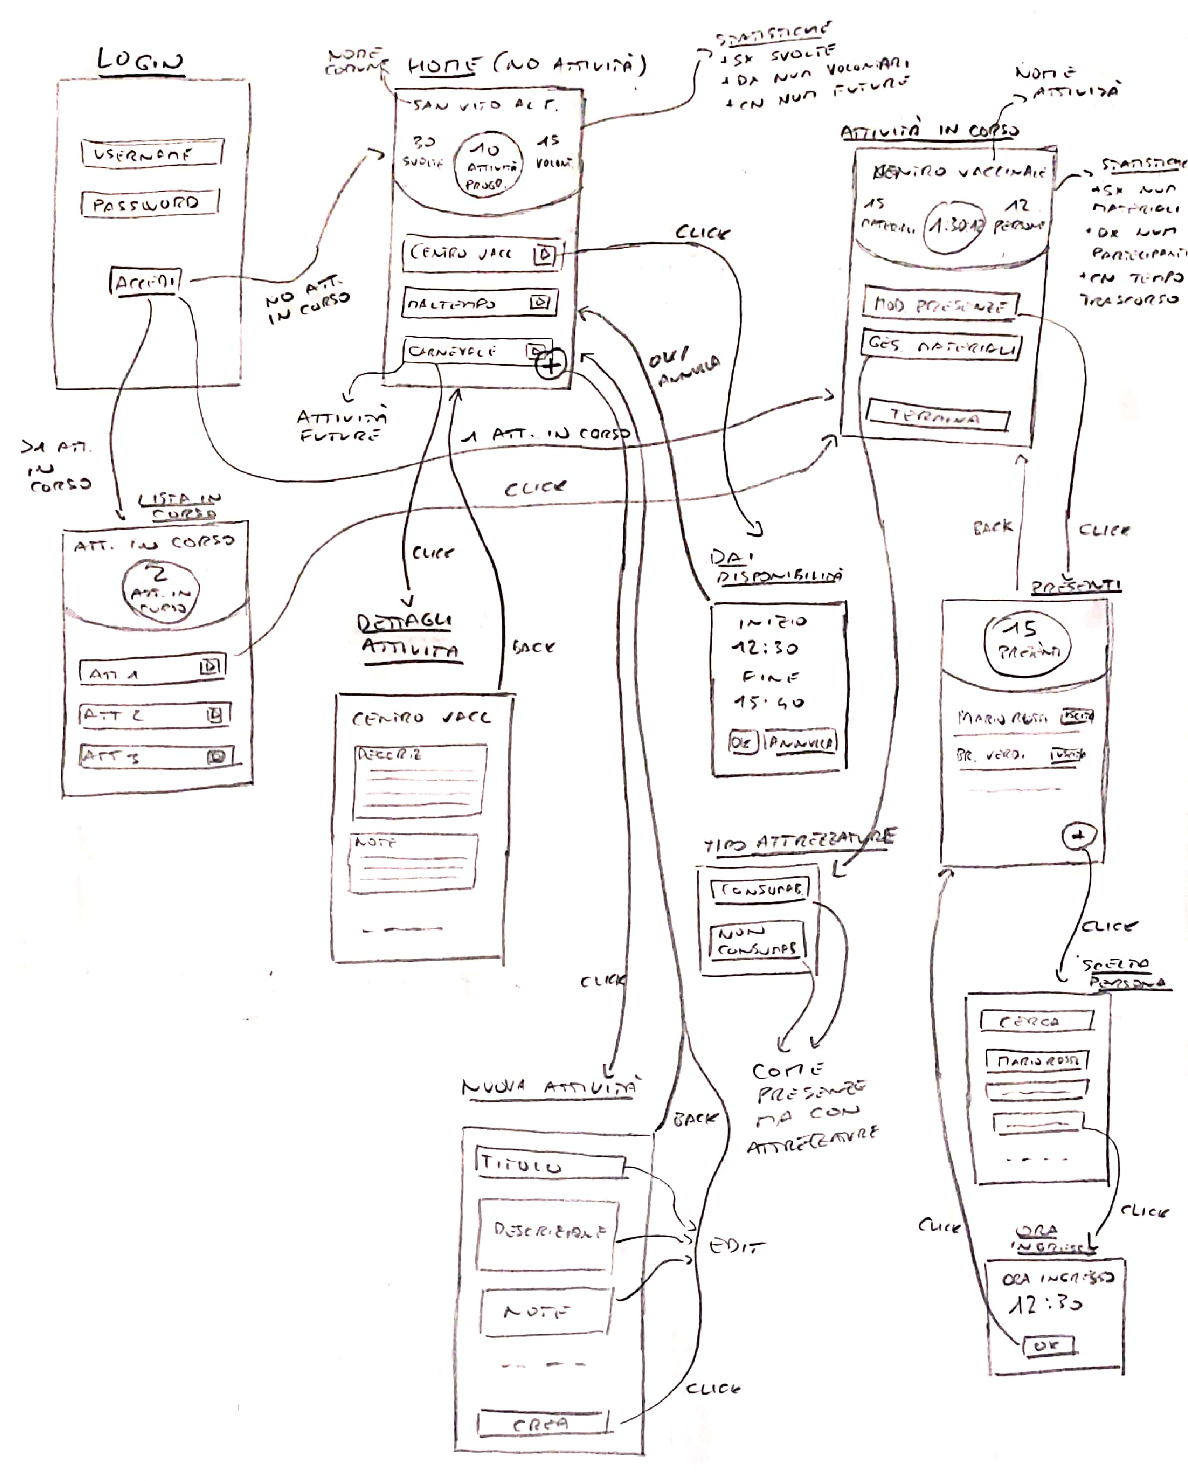
\includegraphics[width=0.8\textwidth]{img/wireframe app.pdf}
    \caption{Wireframe dell'app}
\end{figure}



\subsubsection{Approfondimento: User-centered design}

\paragraph{} Lo \emph{user-centered design} \cite{ucd} è una particolare filosofia di design che incentra la sua attenzione sugli utenti.

\paragraph{} Un punto chiave è il \emph{design partecipato}: gli utilizzatori vengono chiamati a partecipare al processo di design e sviluppo, in modo da dare il loro massimo contributo. Per produrre un'interfaccia che piaccia ad una persona non c'è modo migliore che chiedere a lei stessa!

\paragraph{} Nella prima fase si identificano gli obiettivi: quali sono le competenze degli utilizzatori, qual è l'ambiente di utilizzo, quali sono le richieste specifiche. È importante esaminare queste informazioni, perché per utenti e contesti diversi possono essere adatte interfacce diverse. Ad esempio, una calcolatrice usata da un ingegnere è ben diversa da quella usata da un bambino. 

\paragraph{} La \emph{task analysis} è il processo che analizza attentamente lo svolgimento dei task, per scomporli in azioni fondamentali. Si possono usare diversi livelli di granularità, in base a quale sia lo scopo dell'analisi. 

\paragraph{} L'utilizzo di \emph{mock-up} permette di mostrare all'utente, fin dalla fase di progettazione, quello che sarà l'aspetto del prodotto in modo da poterlo giudicare.

\paragraph{} Gli \emph{scenari} permettono di simulare lo svolgimento delle azioni e l'interazione con il sistema. La sequenza di azioni nello scenario può essere usata per determinare il grafo di transizione tra le schermate.

\paragraph{} L'utilizzo di \emph{guideline} è utile per produrre un'interfaccia consistente con quelle presenti nello stesso contesto. Esistono diversi livelli di guideline: alcuni esempi sono quelle per le app Android, quelle per le app iOS, quelle per applicazioni desktop Windows. Inoltre permettono di riutilizzare componenti standard, in modo da non dover "reinventare la ruota". 

\paragraph{} Le valutazioni basate sull'\emph{osservazione degli utenti} permettono agli sviluppatori di avere un ottimo \emph{feedback} sull'interfaccia che hanno sviluppato, in modo da poterla migliorare.

\begin{figure}[H]
    \centering
    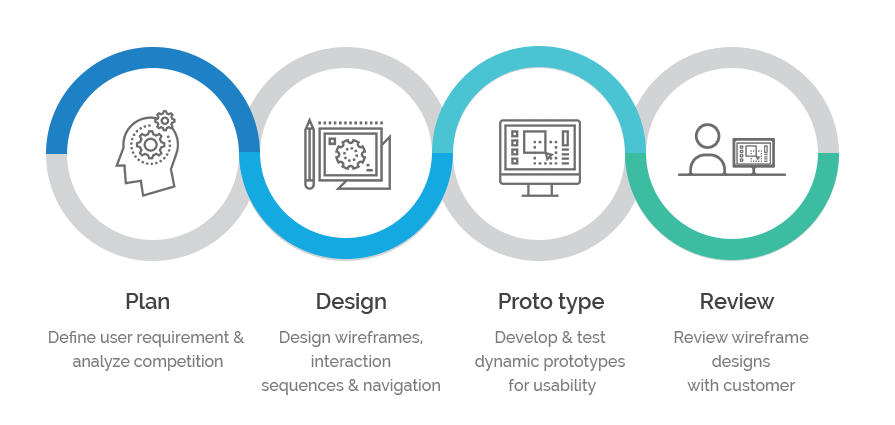
\includegraphics[width=0.8\textwidth]{img/user-centered-design.png}
    \caption{User-centered design}
\end{figure}

\subsection{Progettazione}

\paragraph{} Come piattaforma di sviluppo è stato scelto di utilizzare il framework \emph{React Native} \cite{react_n}. Esso permette di codificare una volta sola per ottenere contemporaneamente una versione adatta ad \emph{Android} e una ad \emph{iOS}. 

\paragraph{} L'unità principale di sviluppo con React Native è il \emph{componente}. In genere, ad ogni schermata dell'app corrisponde un componente diverso. In più, la singola schermata può essere suddivisa gerarchicamente in componenti: una lista di attività, un elemento di questa lista, un'immagine, ecc \dots

\paragraph{} Per ogni schermata, è stata definita la gerarchia dei suoi componenti. Di seguito un esempio. 

\begin{figure}[H]
    \centering
    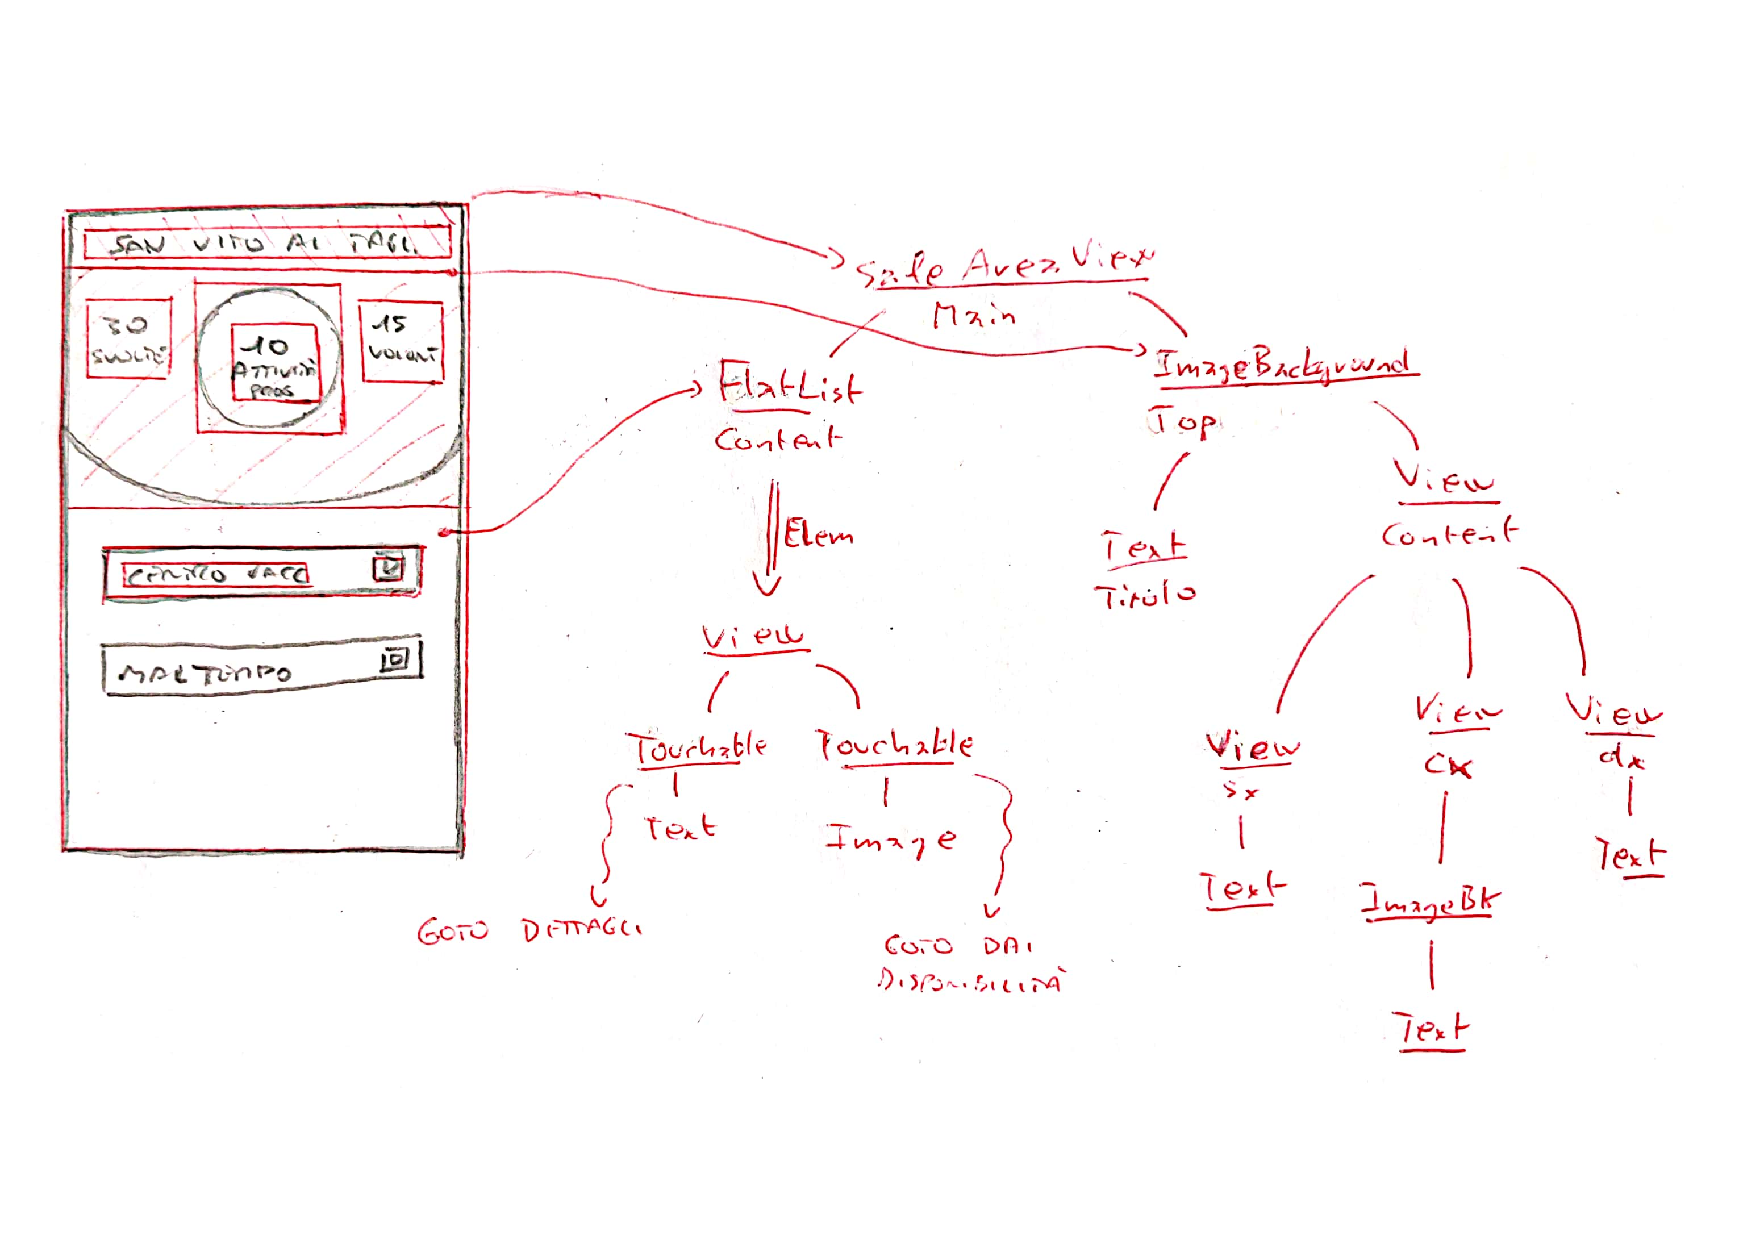
\includegraphics[width=0.8\textwidth]{img/componenti home.pdf}
    \caption{Gerarchia schermata "Home\_no\_attivita"}
\end{figure}

\paragraph{} I componenti si compongono utilizzando l'inclusione. Il componente padre configura i componenti figli tramite il passaggio di dati mediante \emph{props}. I figli interagiscono verso il padre mediante l'esecuzione di \emph{callback}.

\paragraph{} Secondo il principio di \emph{single source of truth}, ogni dato va mantenuto in un solo luogo, che diventa la \emph{"sola e unica fonte di verità"}. Ciò permette di evitare duplicazioni dei dati, con conseguenti perdite di consistenza. 

\paragraph{} Ogni dato va salvato nel \emph{least common ancestor} dei componenti che lo usano. L'hook \emph{val, setter = useState(initVal)}, richiamato dal componente che memorizza il dato, permette di ottenerne getter e setter sotto forma di callback, i quali sono passati ai figli che ne hanno bisogno.

\paragraph{} Per ogni componente, sono stati elencati i dati da esso utilizzati. A seguire un esempio. 

\begin{figure}[H]
    \centering
    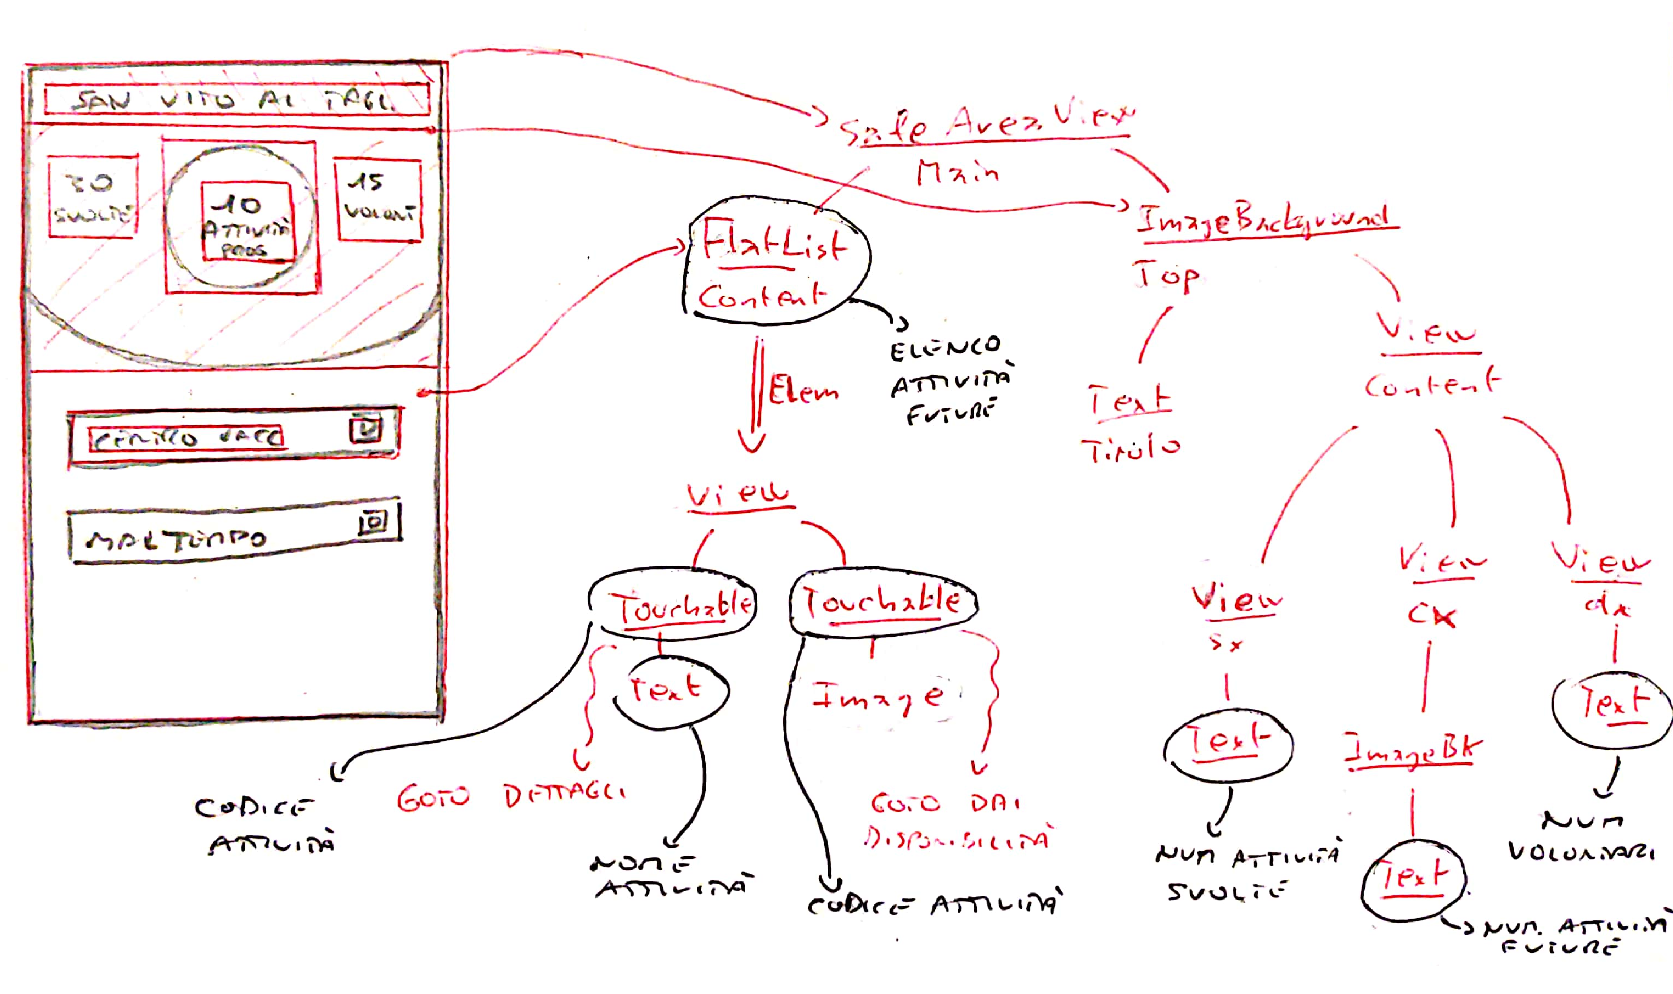
\includegraphics[width=0.8\textwidth]{img/componenti home dati.pdf}
    \caption{Dati utilizzati dai componenti di "Home\_no\_attivita"}
\end{figure}

\paragraph{} È stato creato un componente che gestisce la navigazione principale, il quale contiene tutti i componenti della sidebar individuati nella fase di design.

\paragraph{} Per gestire la navigazione delle singole sezioni, si è deviso di utilizzare degli \emph{StackNavigator}. Essi permettono di utilizzate il pulsante "indietro" per navigare all'ìndietro, pratica comune sia in Android che iOS.  

\begin{figure}[H]
    \centering
    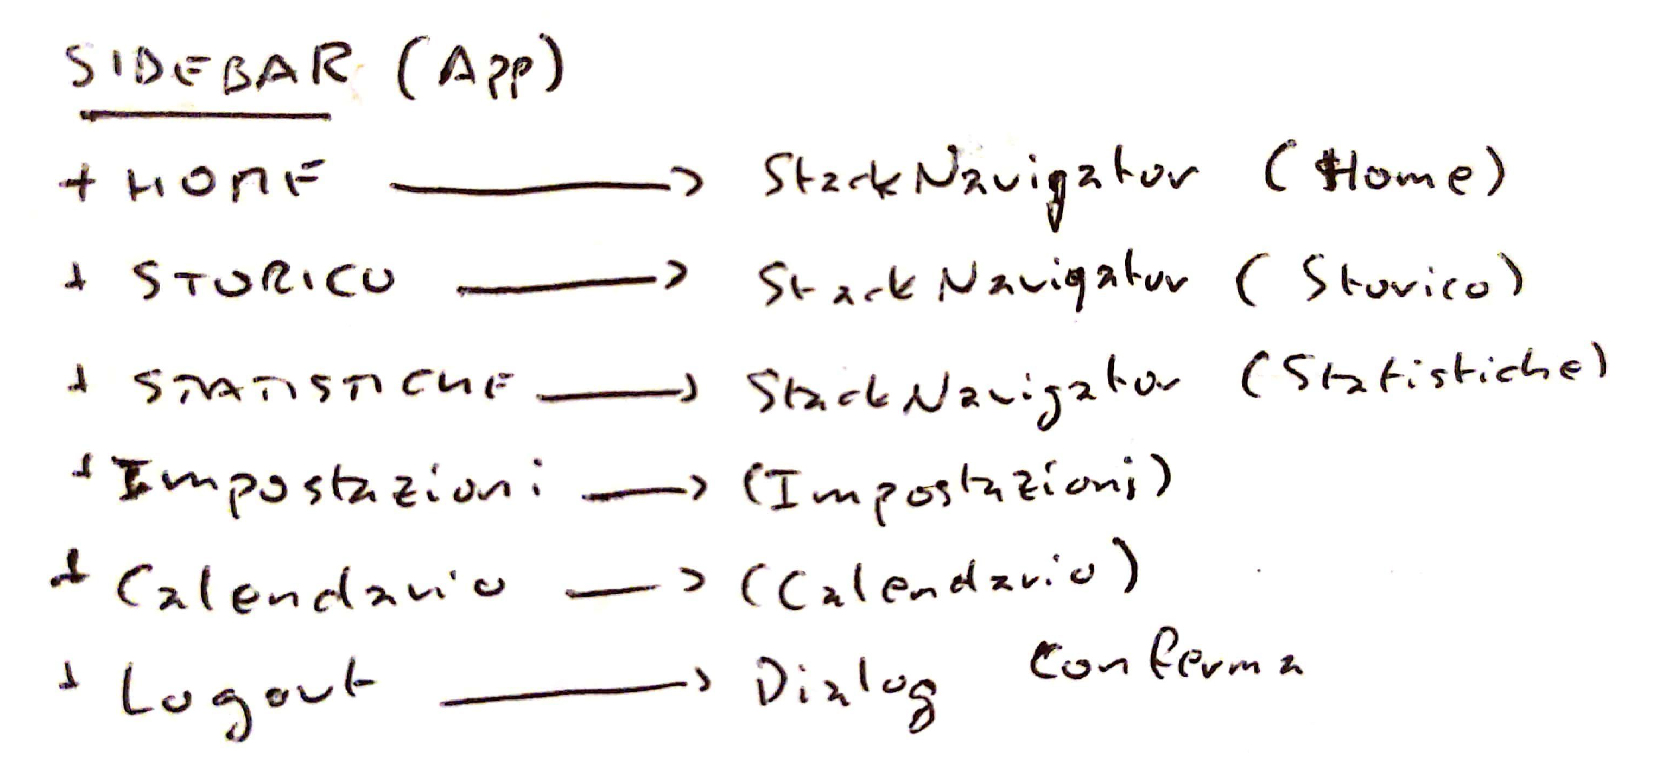
\includegraphics[width=0.8\textwidth]{img/navigation.pdf}
    \caption{Struttura navigazione principale}
\end{figure}



\subsection{Implementazione}

\paragraph{} Una volta terminata la progettazione di una schermata, è possibile passare alla sua implementazione. 

\paragraph{} Il primo passaggio consiste nel creare un nuovo file, il quale conterrà il codice relativo al nuovo componente. Vengono inanzitutto scritti gli import e la struttura di base del componente.

\paragraph{} Come prima cosa si implementa l'interfaccia utente, seguendo la decomposizione in moduli definita nella fase di progettazione. 

\paragraph{} In questa fase i dati vengono inseriti direttamente nel sorgente, in quanto servono solamente per avere una prima resa grafica. 

\paragraph{} I componenti sono grezzi, privi di dettagli. Vengono scelti colori di sfondo contrastanti per avere una buona identificazione di dove si trova ciascun componente. 

\begin{figure}[H]
    \centering
    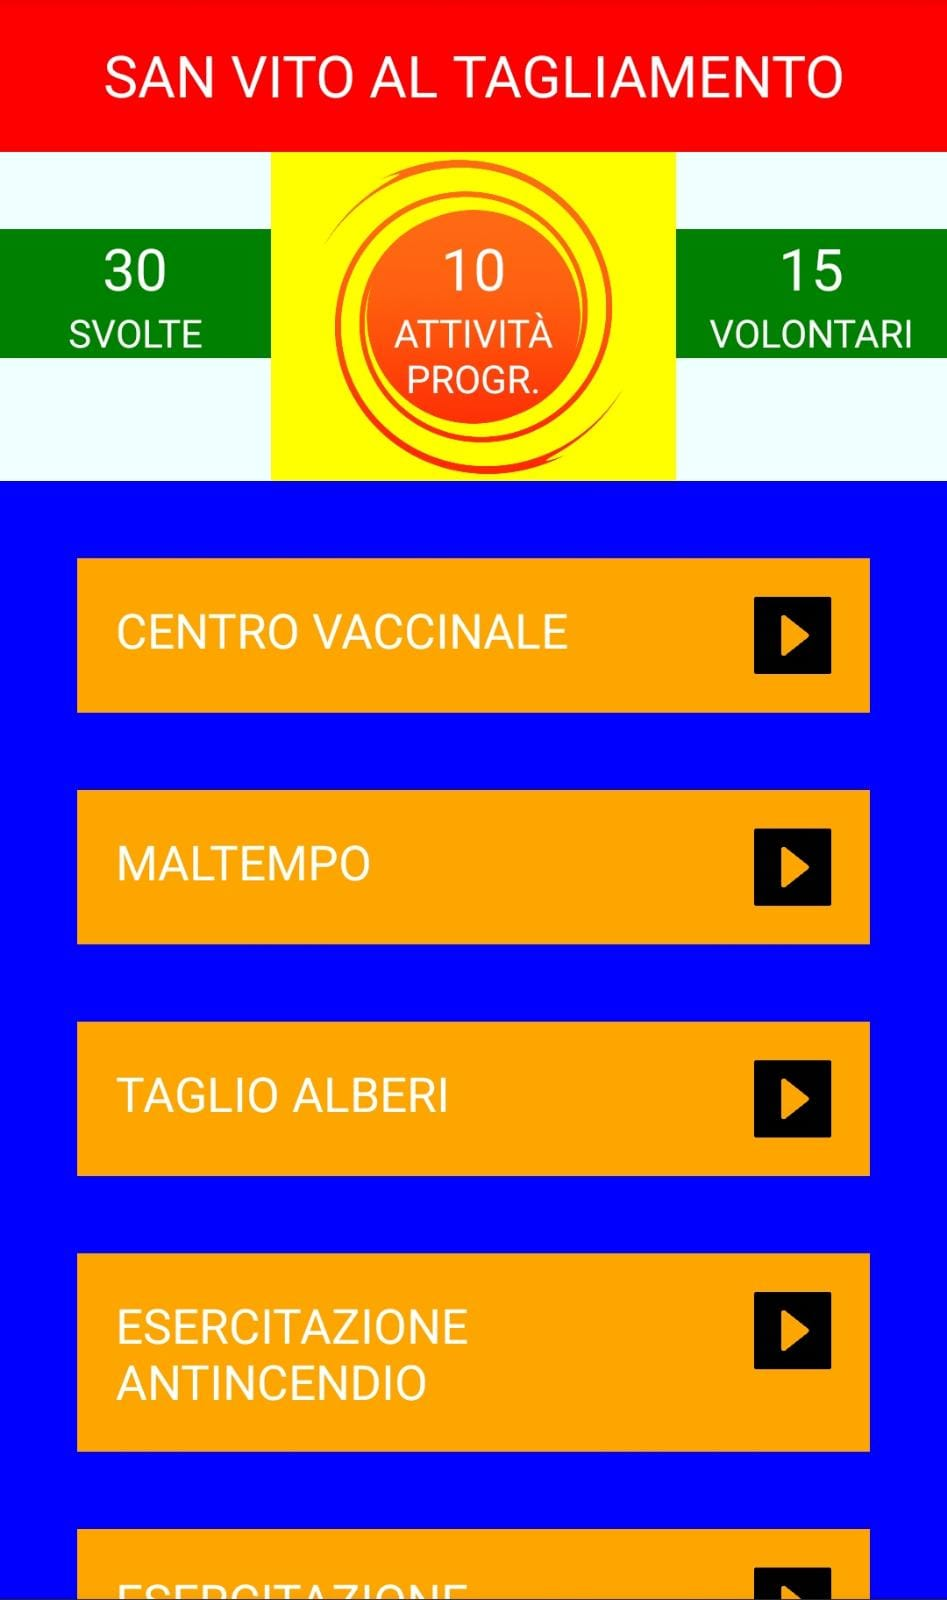
\includegraphics[width=0.4\textwidth]{img/app_1.jpeg}
    \caption{Prima versione della schermata - i dati sono finti}
\end{figure}

\paragraph{} Una volta inclusi e testati tutti i componenti, si passa alla visualizzazione di dati "veri". 

\paragraph{} Per caricare i dati dall'API si usa un \emph{test driver}: un modulo di codice che simula la presenza di un chiamante e che carica i dati in modo "statico" (ad esempio, per caricare la lista delle attività viene usato un token di accesso generato esternamente all'app, ma solo inserito nel codice, in quanto dovrebbe essere generato dalla schermata di login). 

\begin{figure}[H]
    \centering
    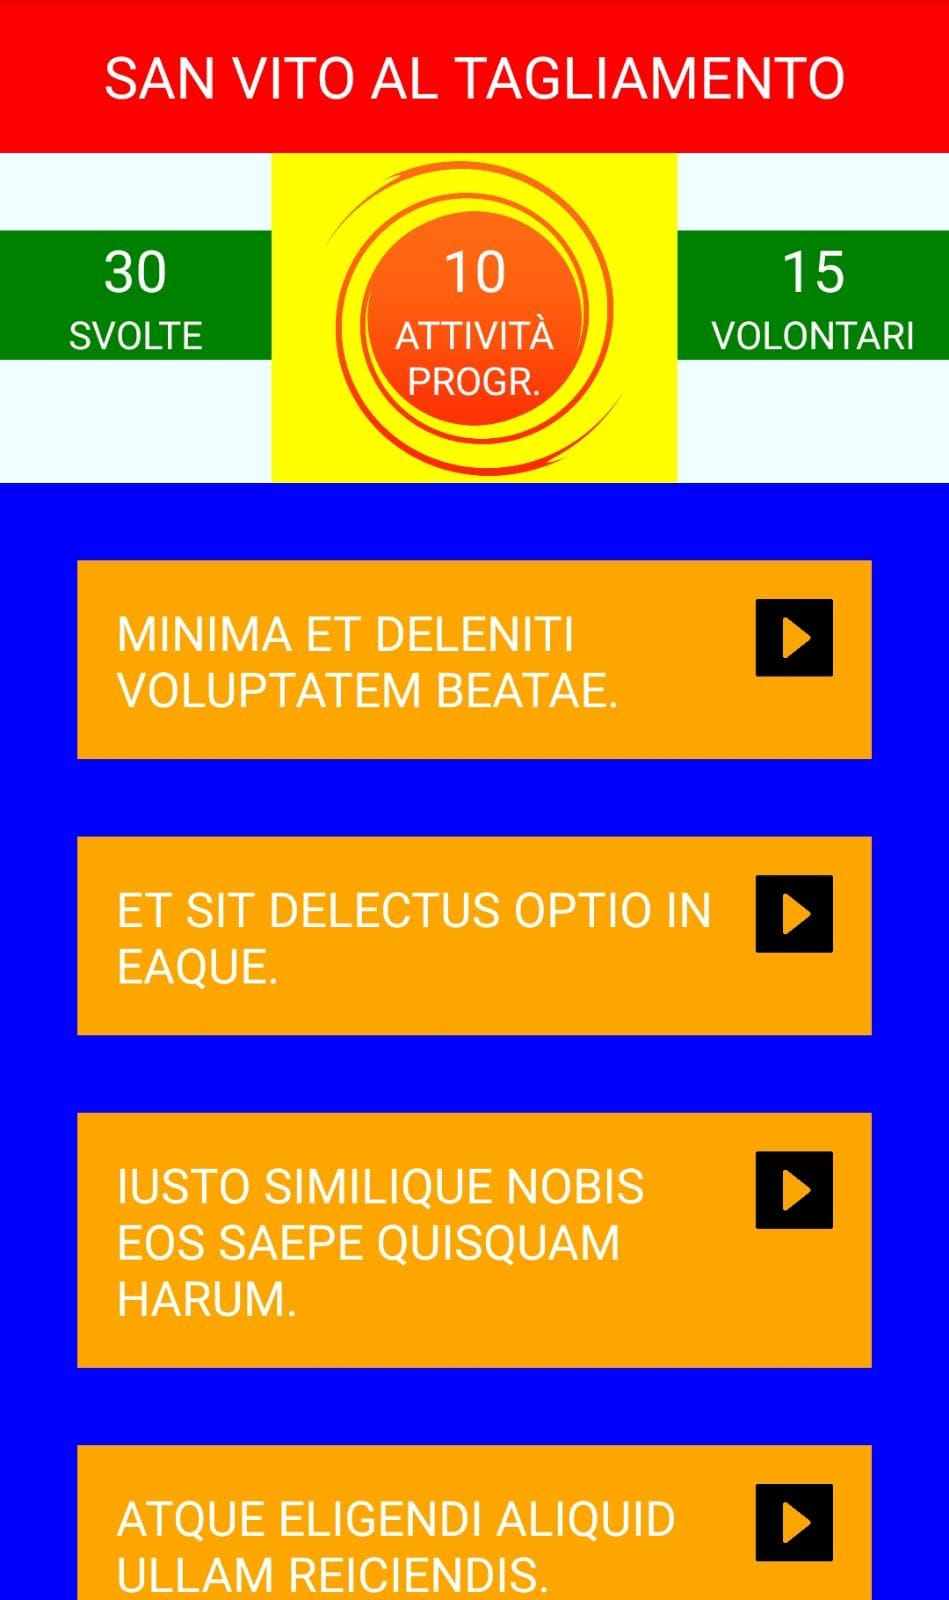
\includegraphics[width=0.4\textwidth]{img/app_2.jpeg}
    \caption{I dati sono caricati dall'API}
\end{figure}

\paragraph{} A questo punto si implementano i gestori degli eventi, come ad esempio il click su un elemento della lista. Questi gestori inizialmente mostrano solo un messaggio di avviso; in un secondo momento inviano i dati al server (se necessario) e usano l'interfaccia di navigazione per passare alla prossima schermata.

\paragraph{} Si rifiniscono quindi i colori e dettagli grafici per ottenere la versione finita del componente. 

\begin{figure}[H]
    \centering
    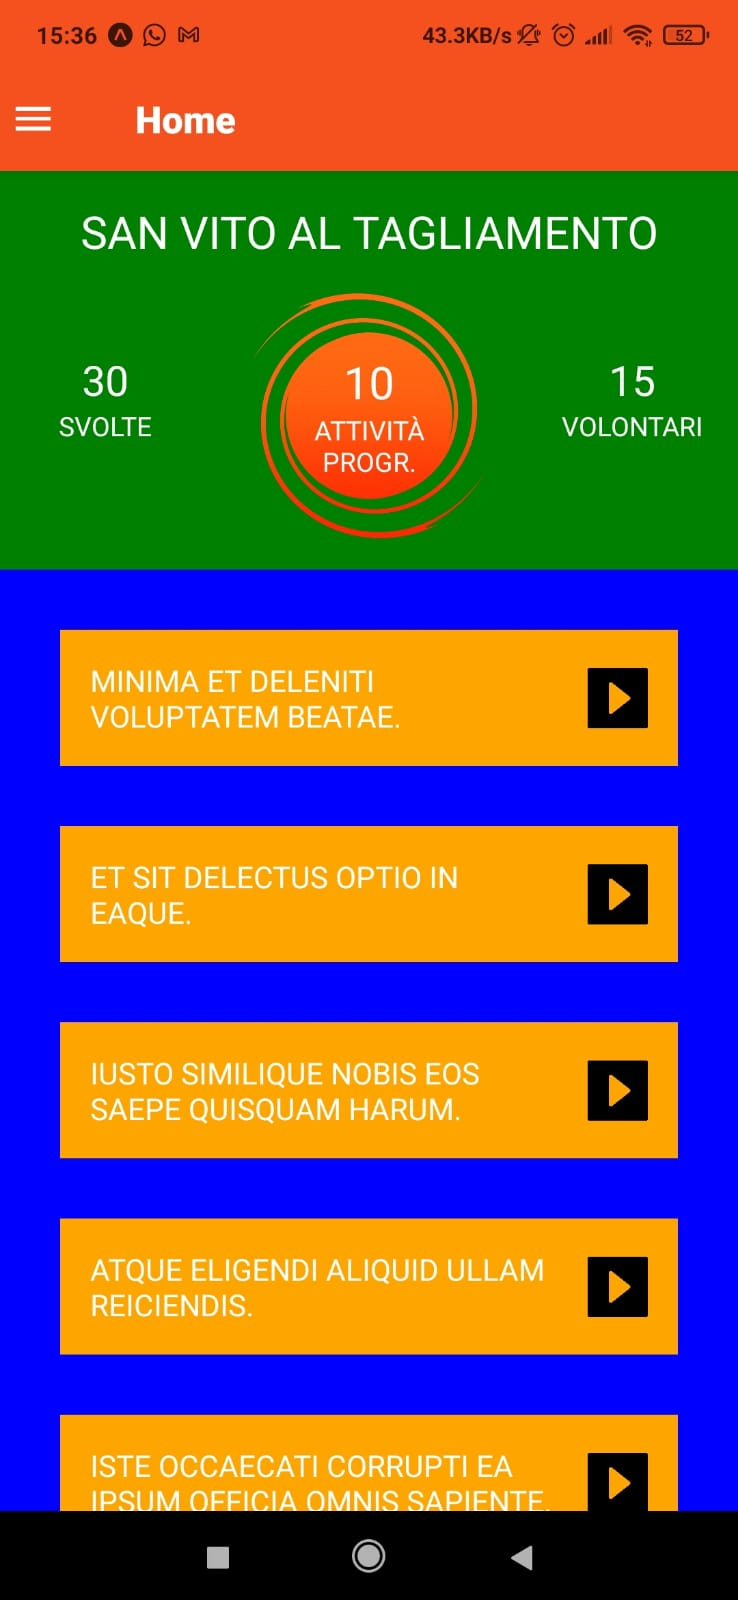
\includegraphics[width=0.4\textwidth]{img/app_3.jpeg}
    \caption{Scelta colori e dettagli grafici}
\end{figure}

\paragraph{} Nell'ultima fase il test driver viene rimosso e la schermata viene integrata assieme al resto dell'app. 

\paragraph{} Ad ogni integrazione, una approfondita fase di test mira a rimuovere tutti i difetti. Prima vengono eseguite le correzioni, più è probabile che esse siano circoscritte (non si diffondano ad altri componenti).

\subsection{Testing}

\paragraph{} Il testing dell'app è stato effettuato tramite la piattaforma Expo \cite{expo}. Essa permette di mettere in comunicazione il dispositivo mobile con il server di sviluppo, caricando automaticamente tutte le modifiche \emph{on-the-fly} e gestendo il \emph{logging/debugging}.

\paragraph{} La connessione può avvenire sia su rete locale, sia da remoto (tramite tunnel pubblico creato da Expo verso il dispositivo di sviluppo). In questo modo è possibile eseguire ed esaminare il comportamento dell'app direttamente sul dispositivo del committente o di un tester specializzato.  

\begin{figure}[H]
    \centering
    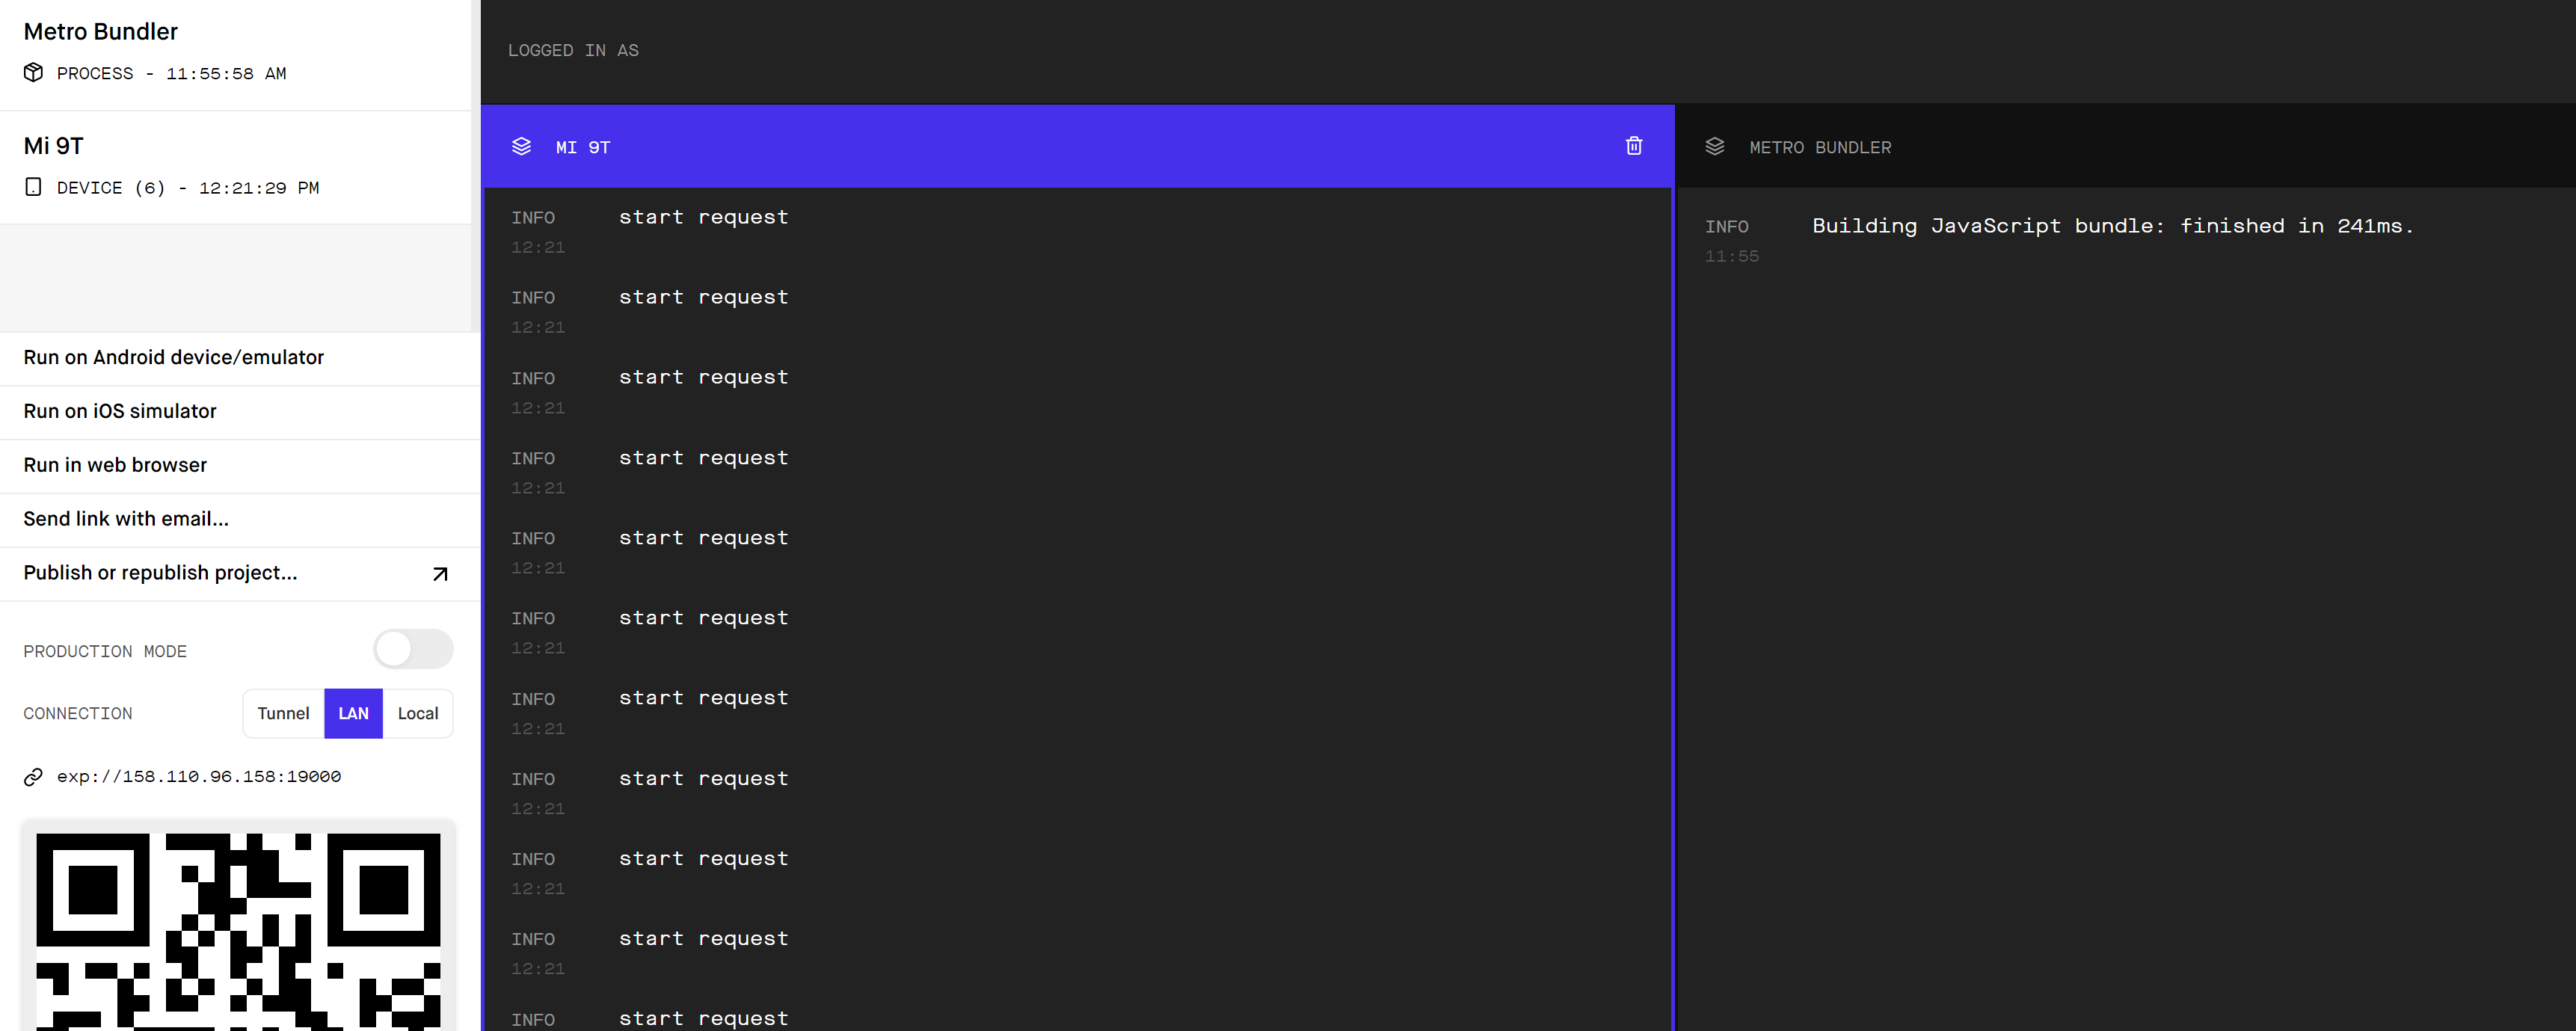
\includegraphics[width=0.9\textwidth]{img/debug_app_pc.png}
    \caption{Testing - Dispositivo di sviluppo}
\end{figure}

\begin{figure}[H]
    \centering
    \begin{subfigure}{.4\textwidth}
      \centering
      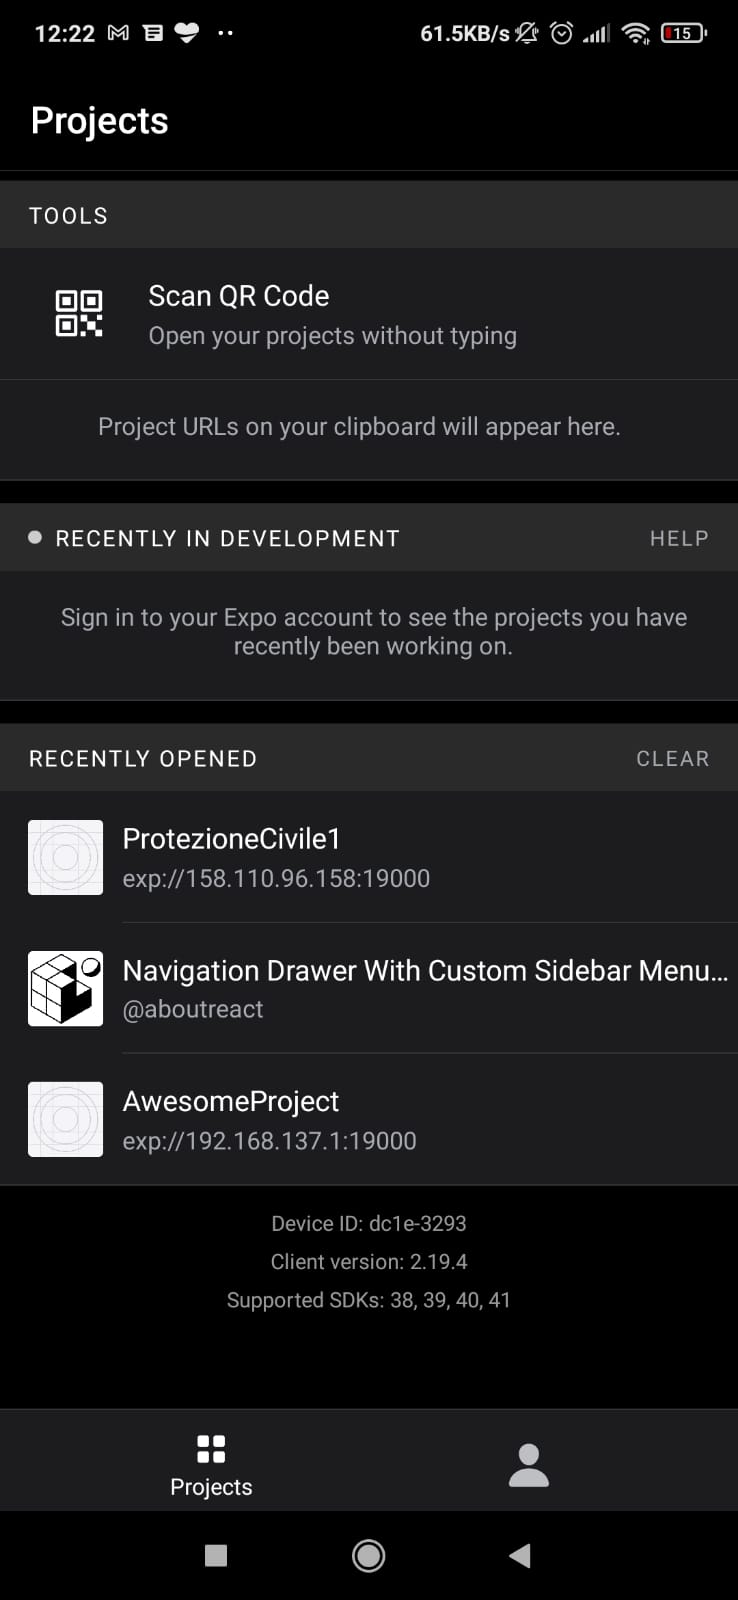
\includegraphics[width=0.8\linewidth]{img/debug_app_1.jpeg}
      \caption{App Expo}
    \end{subfigure}%
    \begin{subfigure}{.4\textwidth}
      \centering
      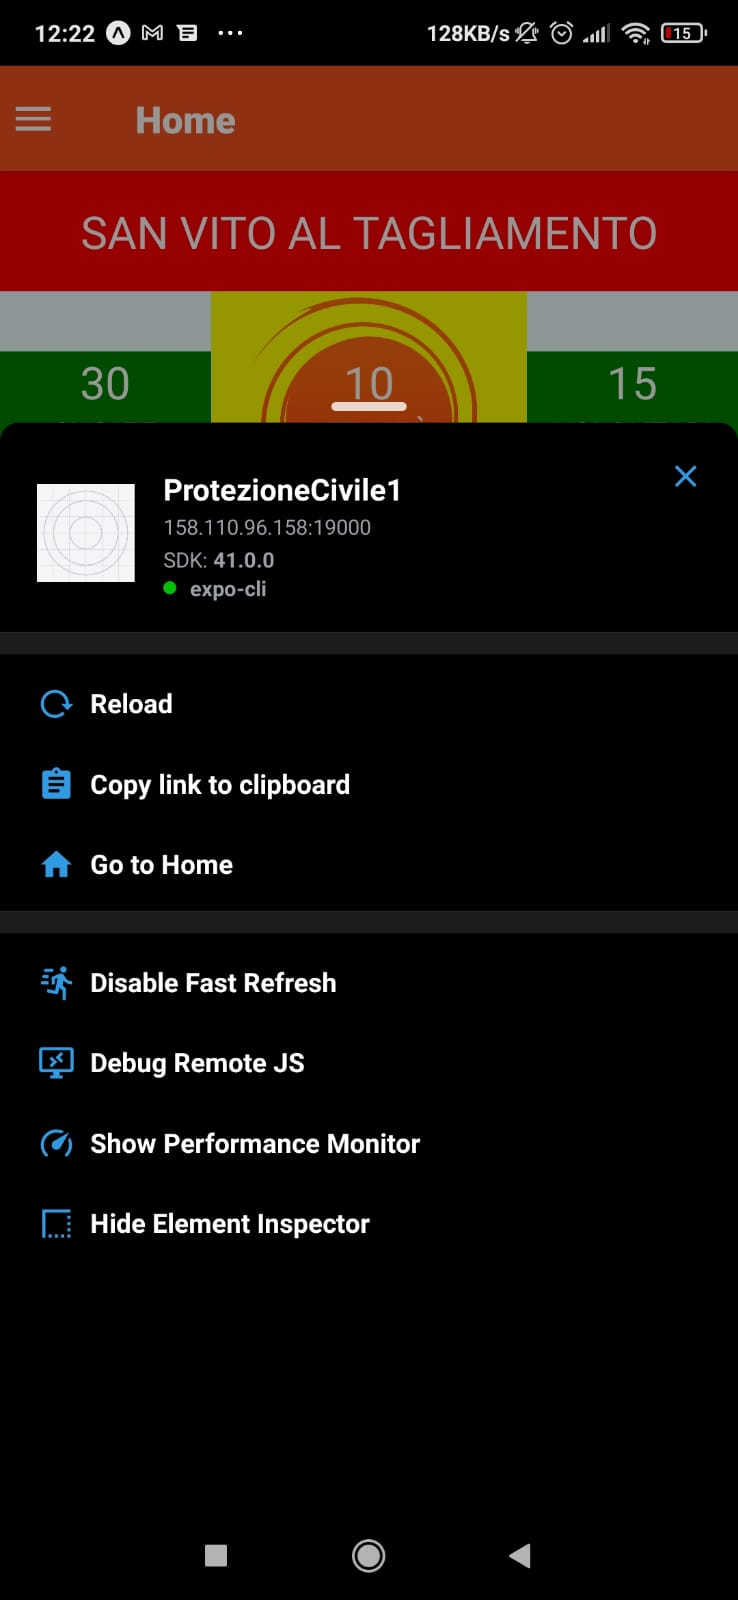
\includegraphics[width=0.8\linewidth]{img/debug_app_2.jpeg}
      \caption{Opzioni di debugging con Expo}
    \end{subfigure}
    \caption{Testing - dispositivo mobile}
\end{figure}

\paragraph{} Sempre utilizzando Expo, è possibile pubblicare i propri progetti sul web. Basta compilare un breve form contenente nome dell'app e dati dello sviluppatore affinché Expo metta a disposizione automaticamente uno spazio in cloud. 

\section{Website}

\paragraph{} Questo capitolo si occuperà del processo di sviluppo del sito web. 

\paragraph{} Sebbene esso sia utilizzato meno frequentemente dell'app, e per questo necessiti di minor cura dei dettagli, è comunque importante rispettare quanto stabilito nella \emph{politica di qualità}. Infatti, pur avendo un'interfaccia meno personalizzata, deve comunque essere utilizzabile con estrema semplicità (personale non specializzato) ed efficienza.

\subsection{Struttura}

\paragraph{} Il website è stato ulteriormente diviso in due parti: \emph{frontend} e \emph{backend} \cite{frontend_vs_backend}. 

\paragraph{} Il \emph{backend} viene eseguito da un server web e si occupa di inviare al client le pagine da esso richieste. 

\paragraph{} Il \emph{frontend} viene eseguito all'interno del browser. Esso è composto da un sorgente di pagina (HTML), da un documento di stile (CSS) e da un insieme di script (JavaScript). 

\paragraph{} Nel caso di questo progetto, il backend genera soltanto la struttura della pagina, mentre i dati vengono richiesti alle API dal frontend (mediante \emph{Ajax} \cite{ajax}). Questo per alleggerire il carico del server, che si limita a servire pagine statiche, e sfruttare le API già scritte per l'utilizzo da parte dell'App. 

\paragraph{} La libreria utilizzata per gestire la grafica è \emph{Bootstrap} \cite{bootstrap}. Essa è una tra le più attualmente utilizzate e supportate dalla community.

\paragraph{} La libreria \emph{jQuery} \cite{jquery} invece è ottima per implementare la parte dinamica della pagina, permettendo di effettuare richieste ajax e manipolare il \emph{DOM}\footnote{Il \emph{Document Object Model} è un'interfaccia ad albero che, all'interno di un browser web, permette l'interazione con i contenuti della pagina.}.


\subsection{Design}

\paragraph{} Il primo passaggio della fase di design del sito web è, come nel caso dell'app, l'elencazione dei task che esso deve essere in grado di svolgere. 

\paragraph{} I task individuati sono i seguenti:
\begin{enumerate}
    \item Creazione/modificazione/eliminazione di \emph{persone}\footnote{Si ricorda che con \emph{persona} si intende un membro tesserato appartenente al gruppo locale di protezione civile.};
    \item Creazione/modificazione/eliminazione di \emph{abilitazioni};
    \item Creazione/modificazione/eliminazione di \emph{comuni};
    \item Creazione/modificazione/eliminazione di \emph{tipi attività};
    \item Creazione/modificazione/eliminazione di \emph{categorie attrezzatura};
    \item Creazione/modificazione/eliminazione di \emph{attrezzature consumabili};
    \item Creazione/modificazione/eliminazione di \emph{attrezzature non consumabili}.
\end{enumerate}

\paragraph{} Inoltre, per il corretto funzionamento del sito, è necessario introdurre la funzione di \emph{login/logout}.

\paragraph{} Si è scelto di implementare la navigazione utilizzando una \emph{responsive sidebar}. Per ogni task della lista è presente la voce corrispondente nella sidebar. 

\begin{figure}[H]
    \centering
    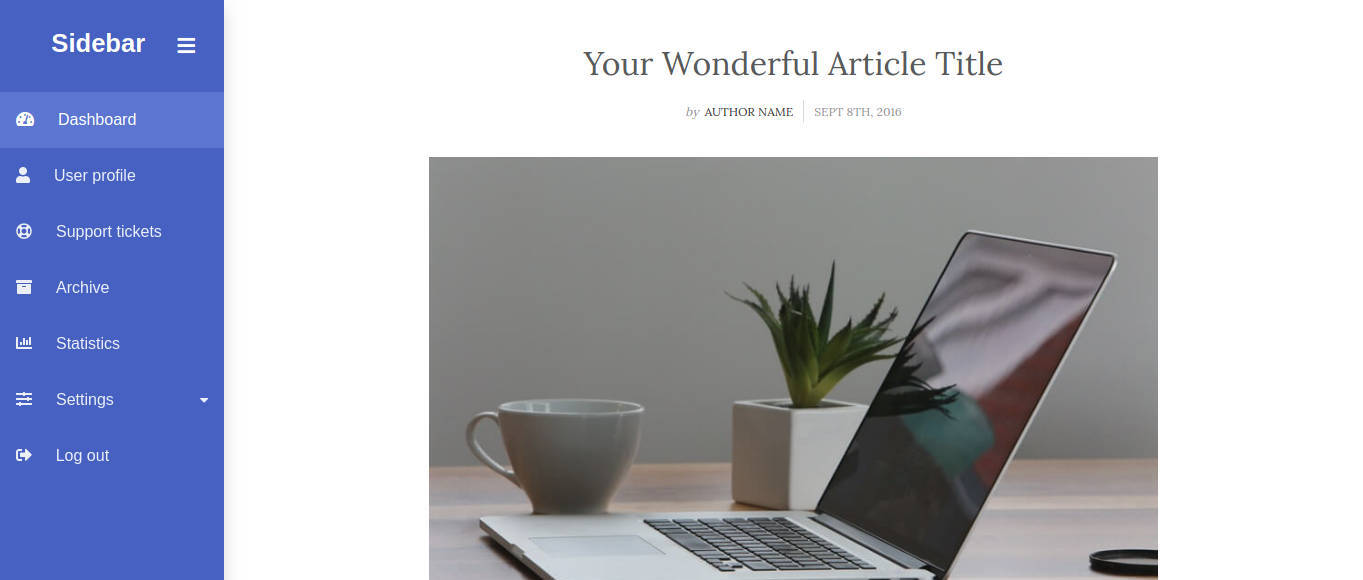
\includegraphics[width=0.8\textwidth]{img/bootstrap-sidebar.jpg}
    \caption{Esempio di navigazione con sidebar}
\end{figure}

\paragraph{} Una volta definita la struttura di navigazione generale, sono stati creati i mockup relativi alle diverse pagine. Essi non devono essere riprodotti con una fedeltà assoluta, ma una loro verosimiglianza consente di valutare in modo migliore l'estetica del prodotto finale. 

\paragraph{} L'apposizione di appunti direttamente nel disegno di mockup permette di specificare meglio il comportamento o l'aspetto di componenti specifiche. 

\begin{figure}[H]
    \centering
    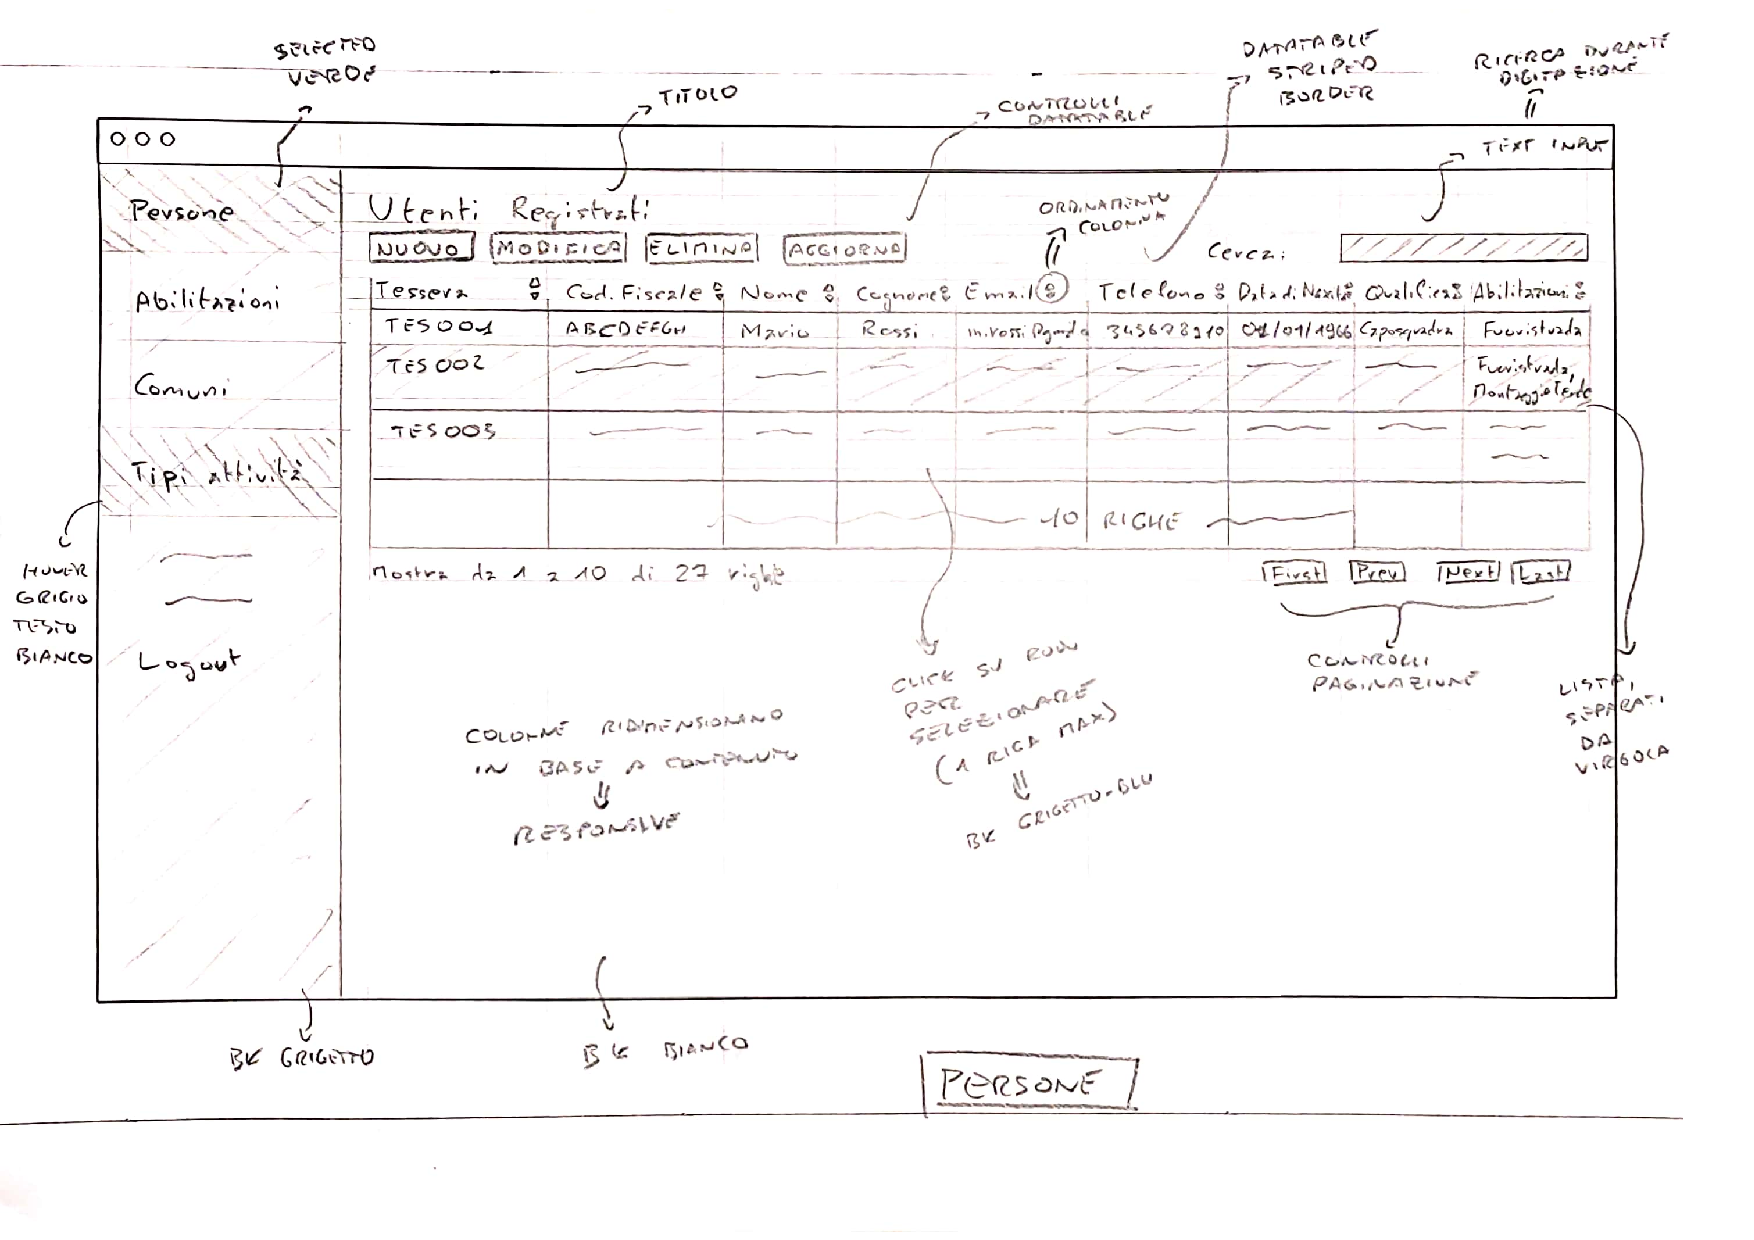
\includegraphics[width=1\textwidth]{img/mockup_web_persone.pdf}
    \caption{Esempio di mockup - pagina persone}
\end{figure}

\paragraph{} I mockup vengono quindi utilizzati per effettuare una progettazione strutturale delle pagine: l'interfaccia viene divisa in componenti, ai componenti principali vengono assegnati dei tag o delle classi css ad-hoc.

\begin{figure}[H]
    \centering
    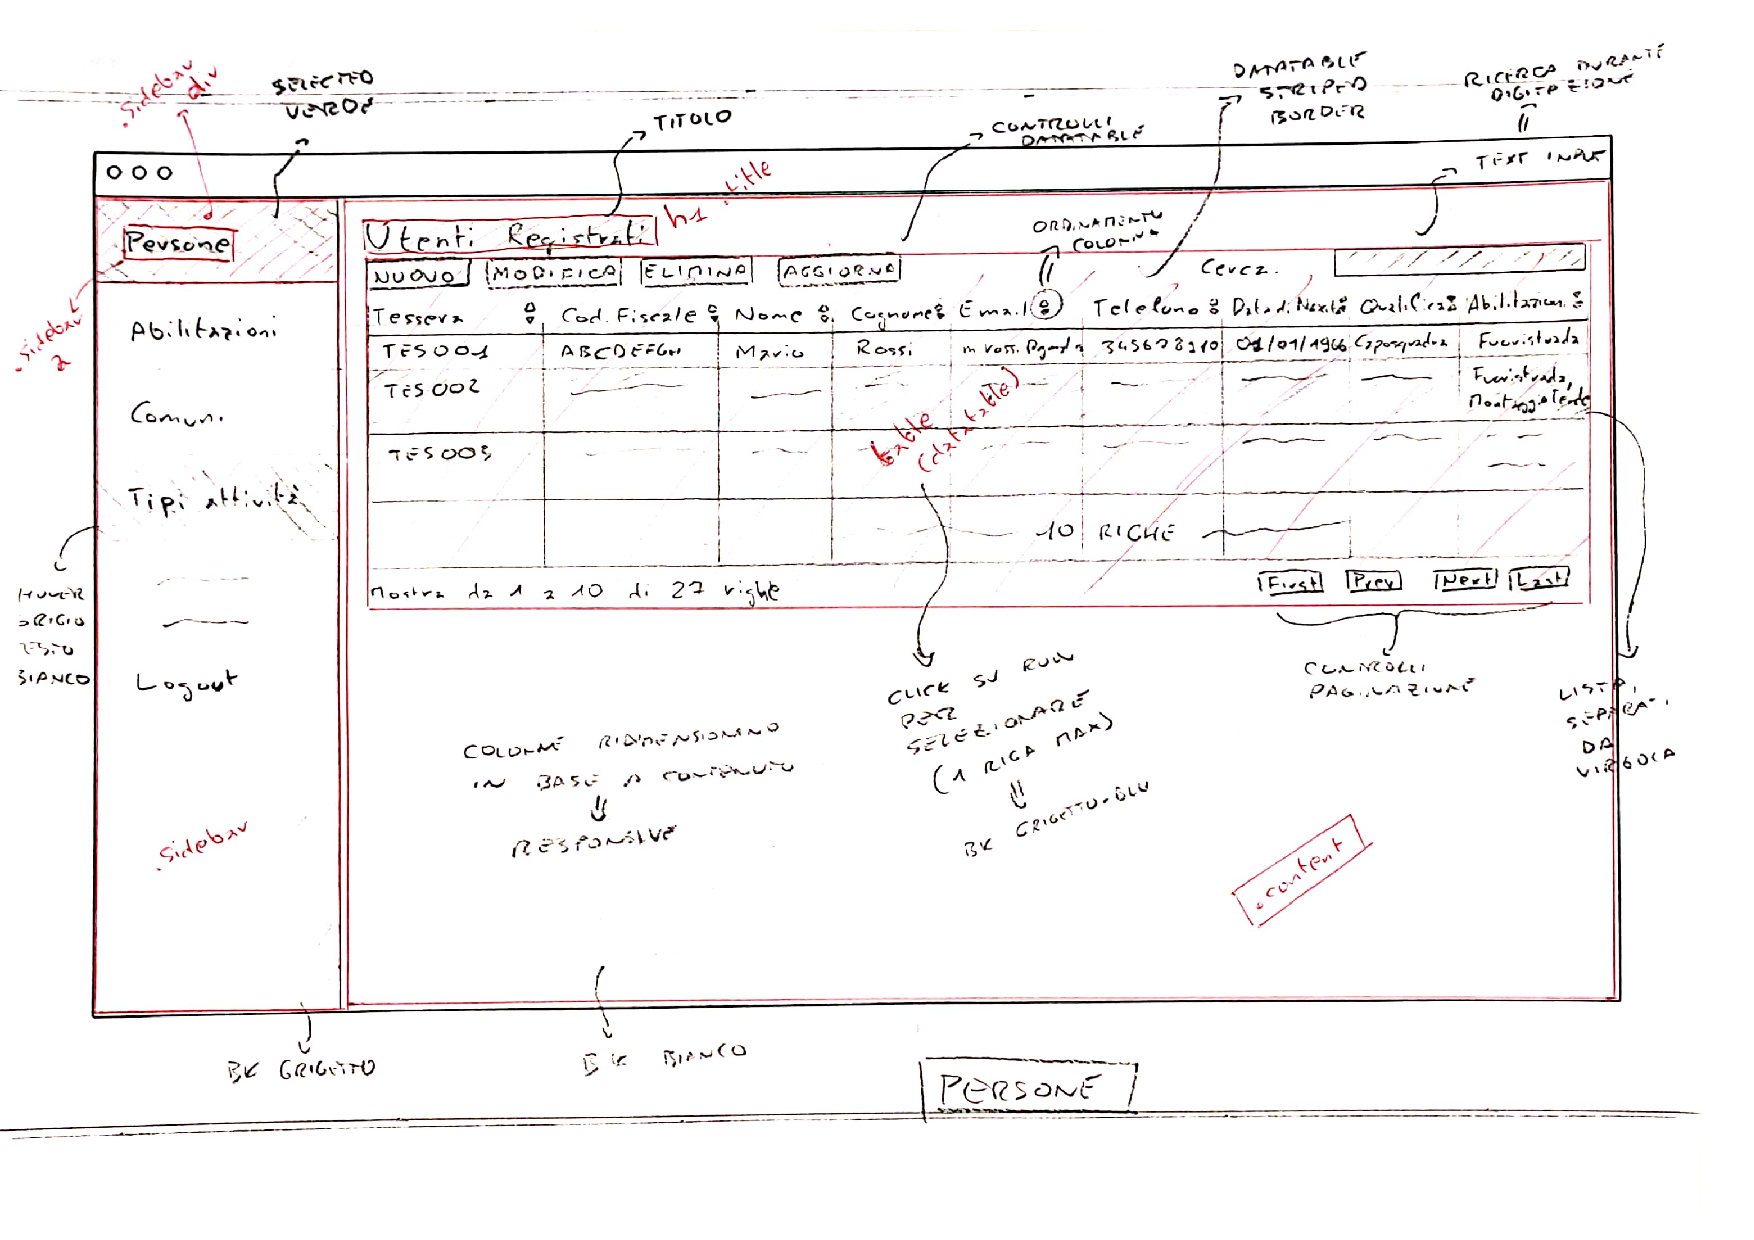
\includegraphics[width=1\textwidth]{img/mockup_web_persone_2.pdf}
    \caption{Esempio di mockup - struttura pagina persone}
\end{figure}

\subsection{Implementazione}

\paragraph{} Per modularizzare il backend, è risultato conveniente sfruttare il \emph{template engine} di Flask, \emph{jinja 2} \cite{jinja}. In questo modo è possibile modificare i contenuti in un solo file per cambiarli in tutte le pagine che lo includono.

\paragraph{} Il template base è quello da cui derivano tutte le pagine. Esso è diviso in moduli: \emph{title} per il titolo della pagina, \emph{includes} per gli script e stylesheet esterni alla pagina, \emph{content} per il contenuto principale della pagina, \emph{scripts} per gli script interni. 

\paragraph{} Oltre alla struttura generale, il template base si occupa anche di richiedere ed effettuare il login dell'utente, se necessario, e di gestire il logout. 

\begin{lstlisting}[language=html, caption=Template base.html]
<!DOCTYPE html>
<html lang="en">
  <head>
    <meta charset="utf-8" />
    ...
    
    <title>
       Protezione Civile San Vito Al Tagliamento 
    </title>
    
    <link
      rel="stylesheet"
      href="https://maxcdn.bootstrapcdn.com/bootstrap/3.3.7/css/bootstrap.css"
    />
    ... altri link a stylesheet ...
    
     
    
    <style>
      #recupera_pw_link {
        float: left;
      }
      .sidebar {
        margin: 0;
        padding: 0;
        width: 200px;
        background-color: #f1f1f1;
        position: fixed;
        height: 100%;
        overflow: auto;
      }
      /* Sidebar links */
      .sidebar a {
        display: block;
        color: black;
        ...
      }
      
      /* On screens that are less than 700px wide, make the sidebar into a topbar */
      @media screen and (max-width: 700px) {
        .sidebar {
          width: 100%;
          height: auto;
          position: relative;
        }
      }
      
      ...altre classi...
      
    </style>
  </head>
  <body>
    <div class="sidebar">
      <a href="/render/persone">Persone</a>
      <a href="/render/abilitazioni">Abilitazioni</a>
      ...altri link...

      <div class="" onclick="logout()">Logout</div>
    </div>
    
    <div class="content pt-5"> </div>

    <div
      class="modal fade"
      id="modal_login"
      tabindex="-1"
      role="dialog"
      aria-labelledby="exampleModalLabel"
      aria-hidden="true"
    >
    
      <!-- dialog login -->
      <div class="modal-dialog" role="document">
        <div class="modal-content">
          <div class="modal-header">
            <h3 class="modal-title" id="exampleModalLabel">
              Effettua l'accesso
            </h3>
        ....
    </div>

    <script
      src="https://code.jquery.com/jquery-3.6.0.min.js"
      integrity="sha256-/xUj+3OJU5yExlq6GSYGSHk7tPXikynS7ogEvDej/m4="
      crossorigin="anonymous"
    ></script>
    ...altri script...

    <script>
      
      $(document).ready(function () {
        //attiva link di pagina corrente
        $(".sidebar a").each(function () {
          if (window.location.href.includes(this.href)) {
            $(this).addClass("active");
          }
        });

        modal_login = $("#modal_login");

        token = Cookies.get("token");
        if (token == null) {
          showLogin();
        }
      });

      //mostra modal login
      function showLogin() {
        Cookies.remove("token");

        modal_login.modal({
          backdrop: false,
          keyboard: false,
        });
      }

      //oggetto contenente i dati inseriti nella login-form
      function getLoginForm() {
        return $("#login-form").serializeJSON();
      }

      function login_click() {
        $.ajax({
          url: "/api/do_login",
          type: "POST",
          dataType: "json",
          contentType: "application/json",
          data: JSON.stringify(getLoginForm()),
        }).success(function (res) {
          if (res.token == null) {
            alert("credenziali errate");
          } else {
            token = res.token;
            Cookies.set("token", token);
            location.reload();
          }
        });
      }

      function logout() {
        $.ajax({
          url: "/api/do_logout",
          ...
          beforeSend: function (request) {
            request.setRequestHeader("Authorization", token);
          },
        }).success(function (res) {
          Cookies.remove("token");
          location.reload();
        });
      }

      function recupera_pw_click() {
        if (!confirm("Vuoi davvero recuperare la tua password?")) return;

        var data = getLoginForm();

        if (data.email == "") {
          alert("inserisci una email");
          return;
        }

        $.ajax({
          url: "/api/richiedi_recupera_pw",
          ...
        }).success(function (res) {
          alert("Ti e' stata inviata una email all'indirizzo specificato");
        });
      }
    </script>

     
  </body>
</html>

\end{lstlisting}

\paragraph{} Il template \emph{base\_table} estende \emph{base}, introducendo una \emph{datatable} generica nella sezione \emph{content}. 

\begin{lstlisting}[language=html, caption=Template base\_table.html]
 


<h1 class="title pb-3">
   Titolo tabella 
</h1>
<table
  cellpadding="0"
  cellspacing="0"
  border="0"
  class="dataTable table table-striped"
  id="example"
></table>


\end{lstlisting}

\paragraph{} A questo punto è possibile creare un template per ogni pagina del sito, il quale implementa la logica dell'applicazione. 

\paragraph{} Le operazioni implementate in ogni template sono:\begin{enumerate}
    \item \emph{Fetch dei dati}, tramite chiamata \emph{ajax};
    \item \emph{Visualizzazione dei dati nella datatable};
    \item \emph{Operazioni sui dati}: create, update, delete, reload.  
\end{enumerate}

\begin{lstlisting}[language=html, caption=Esempio template - persona.html]
 

 Membri registrati  


<script>
  $(document).ready(function() {

      var qualificaOptions = { "caposquadra" : "Caposquadra", "volontario" : "Volontario" , "coordinatore" : "Coordinatore" };
      var permessiOptions = { "crea_evento" : "Gestione eventi", "cms" : "Gestione piattaforma" };
      
      //valore iniettato dal template engine (lato server), in quanto presi dal database
      var abilitazioniOptions = [{{ abilitazioniOptions | safe }}];

      var columnDefs = [
            //utilizzato per update, invisibile all'utente. Contiene il valore di "numero_tessera" prima della modifica.
            {
                data: "numero_tessera_old",
                visible: false,
                searchable: false,
                type: "hidden"
            },
            {
                data: "numero_tessera",
                title: "Tessera",
                unique: true
            },
            {
                data: "codice_fiscale",
                title: "Cod. fiscale",
                unique: true
            },
            ...
            {
                data: "data_di_nascita",
                title: "Data di nascita",
                datetimepicker: { timepicker: false, format : "Y/m/d"}
            },
            {
                //genera select
                data: "qualifica",
                title: "Qualifica",
                type : "select",
                options : qualificaOptions,
                select2 : { width: "100%"},
                render: function (data, type, row, meta) {
                  if (data == null || !(data in qualificaOptions)) return null;
                  return qualificaOptions[data];
                }
            },
            {
                //genera multiselect
                data: "abilitazioni",
                title: "Abilitazioni",
                type: "select",
                options: abilitazioniOptions,
                multiple : true,
                select2 : { width: "100%"},
                render : function (data, type, row, meta) {
                    console.log(data)
                    return data;
                }
            },
            ...
          ];


    //configurazione datatable
    myTable = $('#example').DataTable({
      "sPaginationType": "full_numbers",
      ajax: { //fetch dei dati tramite ajax
        'url': '/api/get_persona',
        'type': 'GET',
        'beforeSend': function (request) {
            request.setRequestHeader("Authorization", token);    //token autorizzazione
        },
        "dataSrc": function ( json ) {
            json.forEach(function(elem) {    //crea copia chiave
                elem["numero_tessera_old"] = elem["numero_tessera"];
            });
            return json;
        },
        error: (response) => {   
            if (response.status == 401){    //se token non valido
                showLogin()
            }else{
                alert(response.responseJSON.message)    //errore generico
            }
        }
      },
      columns: columnDefs,
      dom: 'Bfrtip',        // Needs button container
      select: 'single',
      responsive: true,
      altEditor: true,     // Enable altEditor
      buttons: [{
              text: 'Nuovo',
              name: 'add'        // do not change name
          },
          {
              extend: 'selected', // Bind to Selected row
              text: 'Modifica',
              name: 'edit'        // do not change name
          },
          {
              extend: 'selected', // Bind to Selected row
              text: 'Elimina',
              name: 'delete'      // do not change name
          },
          {
              text: 'Aggiorna dati',
              name: 'refresh'      // do not change name
      }],
      onAddRow: function(datatable, rowdata, success, error) {
          $.ajax({
              url: "/api/create_persona",
              type: 'POST',
              dataType: 'json',
              contentType: 'application/json',
              data: JSON.stringify(rowdata),
              beforeSend: function (request) {
                    request.setRequestHeader("Authorization", token);
                },
              success: function() { rowdata["numero_tessera_old"] = rowdata["numero_tessera"]; success(rowdata); },
              error: function(response) { alert(response.responseJSON.message) }
          });
      },
      onDeleteRow: function(datatable, rowdata, success, error) {
          $.ajax({
              url: "/api/delete_persona",
              type: 'DELETE',
              
              ...
          });
      },
      onEditRow: function(datatable, rowdata, success, error) {
          $.ajax({
              url: "/api/update_persona",
              
              ...
          });
      }
    });

  });
</script>


\end{lstlisting}


\subsubsection{Approfondimento: Template con jinja 2}

\paragraph{} \emph{Jinja 2} \cite{jinja} è un famoso template engine, utilizzato da framework come Flask e Django.

\paragraph{} Un \emph{template engine} è una libreria che si occupa di elaborare particolari file, detti \emph{template}, in modo da produrre un documento risultato. 

\paragraph{} I \emph{template} definiscono una struttura: tramite una particolare sintassi è possibile includere in essi valori, liste o persino altri template. 

\paragraph{} I template risultano quindi particolarmente utili quando si ha una struttura ricorrente. Questo solitamente è il caso delle pagine web, dove le pagine possono essere composte mediante moduli indipendenti e condivisi.

\paragraph{} La sintassi di jinja 2 è molto semplice:
\begin{itemize}
    \item $\{\% ... \%\}$ denota uno statement;
    \item $\{\{ ... \}\}$ denota un'espressione da stampare nell'output;
    \item $\{\# ... \#\}$ denota un commento;
    \item $\# ... \#\#$ denota un line statement.
\end{itemize}

\paragraph{} Di seguito alcuni esempi per comprendere le direttive principali.

\begin{lstlisting}[language=Python, caption=Scrivere il valore di una variabile]
<div> Nome: {{ elemento.nome }} </div>
<div> Nome: {{ foo['bar'] }} </div>
\end{lstlisting}

\begin{lstlisting}[language=Python, caption=Valutare una condizione]

    Errore!

\end{lstlisting}

\begin{lstlisting}[language=Python, caption=Iterare su una lista]

    {{ item }}

\end{lstlisting}

\paragraph{} È anche possibile utilizzare le keyword \emph{extends} e \emph{block} per sfruttare l'ereditarietà in modo da costruire template in modo gerarchico:

\begin{lstlisting}[language=Python, caption=Padre]
<!DOCTYPE html>
<html lang="en">
<head>
    
    <link rel="stylesheet" href="style.css" />
    <title> - My Webpage</title>
    
</head>
<body>
    <div id="content"></div>
    <div id="footer">
        
        &copy; Copyright 2008 by <a href="http://domain.invalid/">you</a>.
        
    </div>
</body>
</html>
\end{lstlisting}


\begin{lstlisting}[language=Python, caption=Figlio]

Index

    {{ super() }}
    <style type="text/css">
        .important { color: #336699; }
    </style>


    <h1>Index</h1>
    <p class="important">
      Welcome to my awesome homepage.
    </p>

\end{lstlisting}

\subsection{Testing}

\paragraph{} Per effettuare il testing durante lo sviluppo, risulta naturale utilizzare il server di test offerto da flask. 

\paragraph{} Ogni client web mostra i contenuti a suo modo. Sebbene HTML5 sia ormai uno standard de facto, è comunque importante verificare il comportamento del sito web su tutti i browser in commercio. Il team di sviluppo ha verificato il funzionamento del website utilizzando \emph{Google Chrome}, \emph{Firefox} e \emph{Microsoft Edge}, aggiornati ad una versione recente.

\paragraph{} La visualizzazione dei conenuti dipende anche dalle dimensioni e risoluzione dello schermo. Per questo motivo è necessario anche effettuare delle prove ridimensionando la finestra e cambiandone la forma. 

\begin{figure}[H]
    \centering
    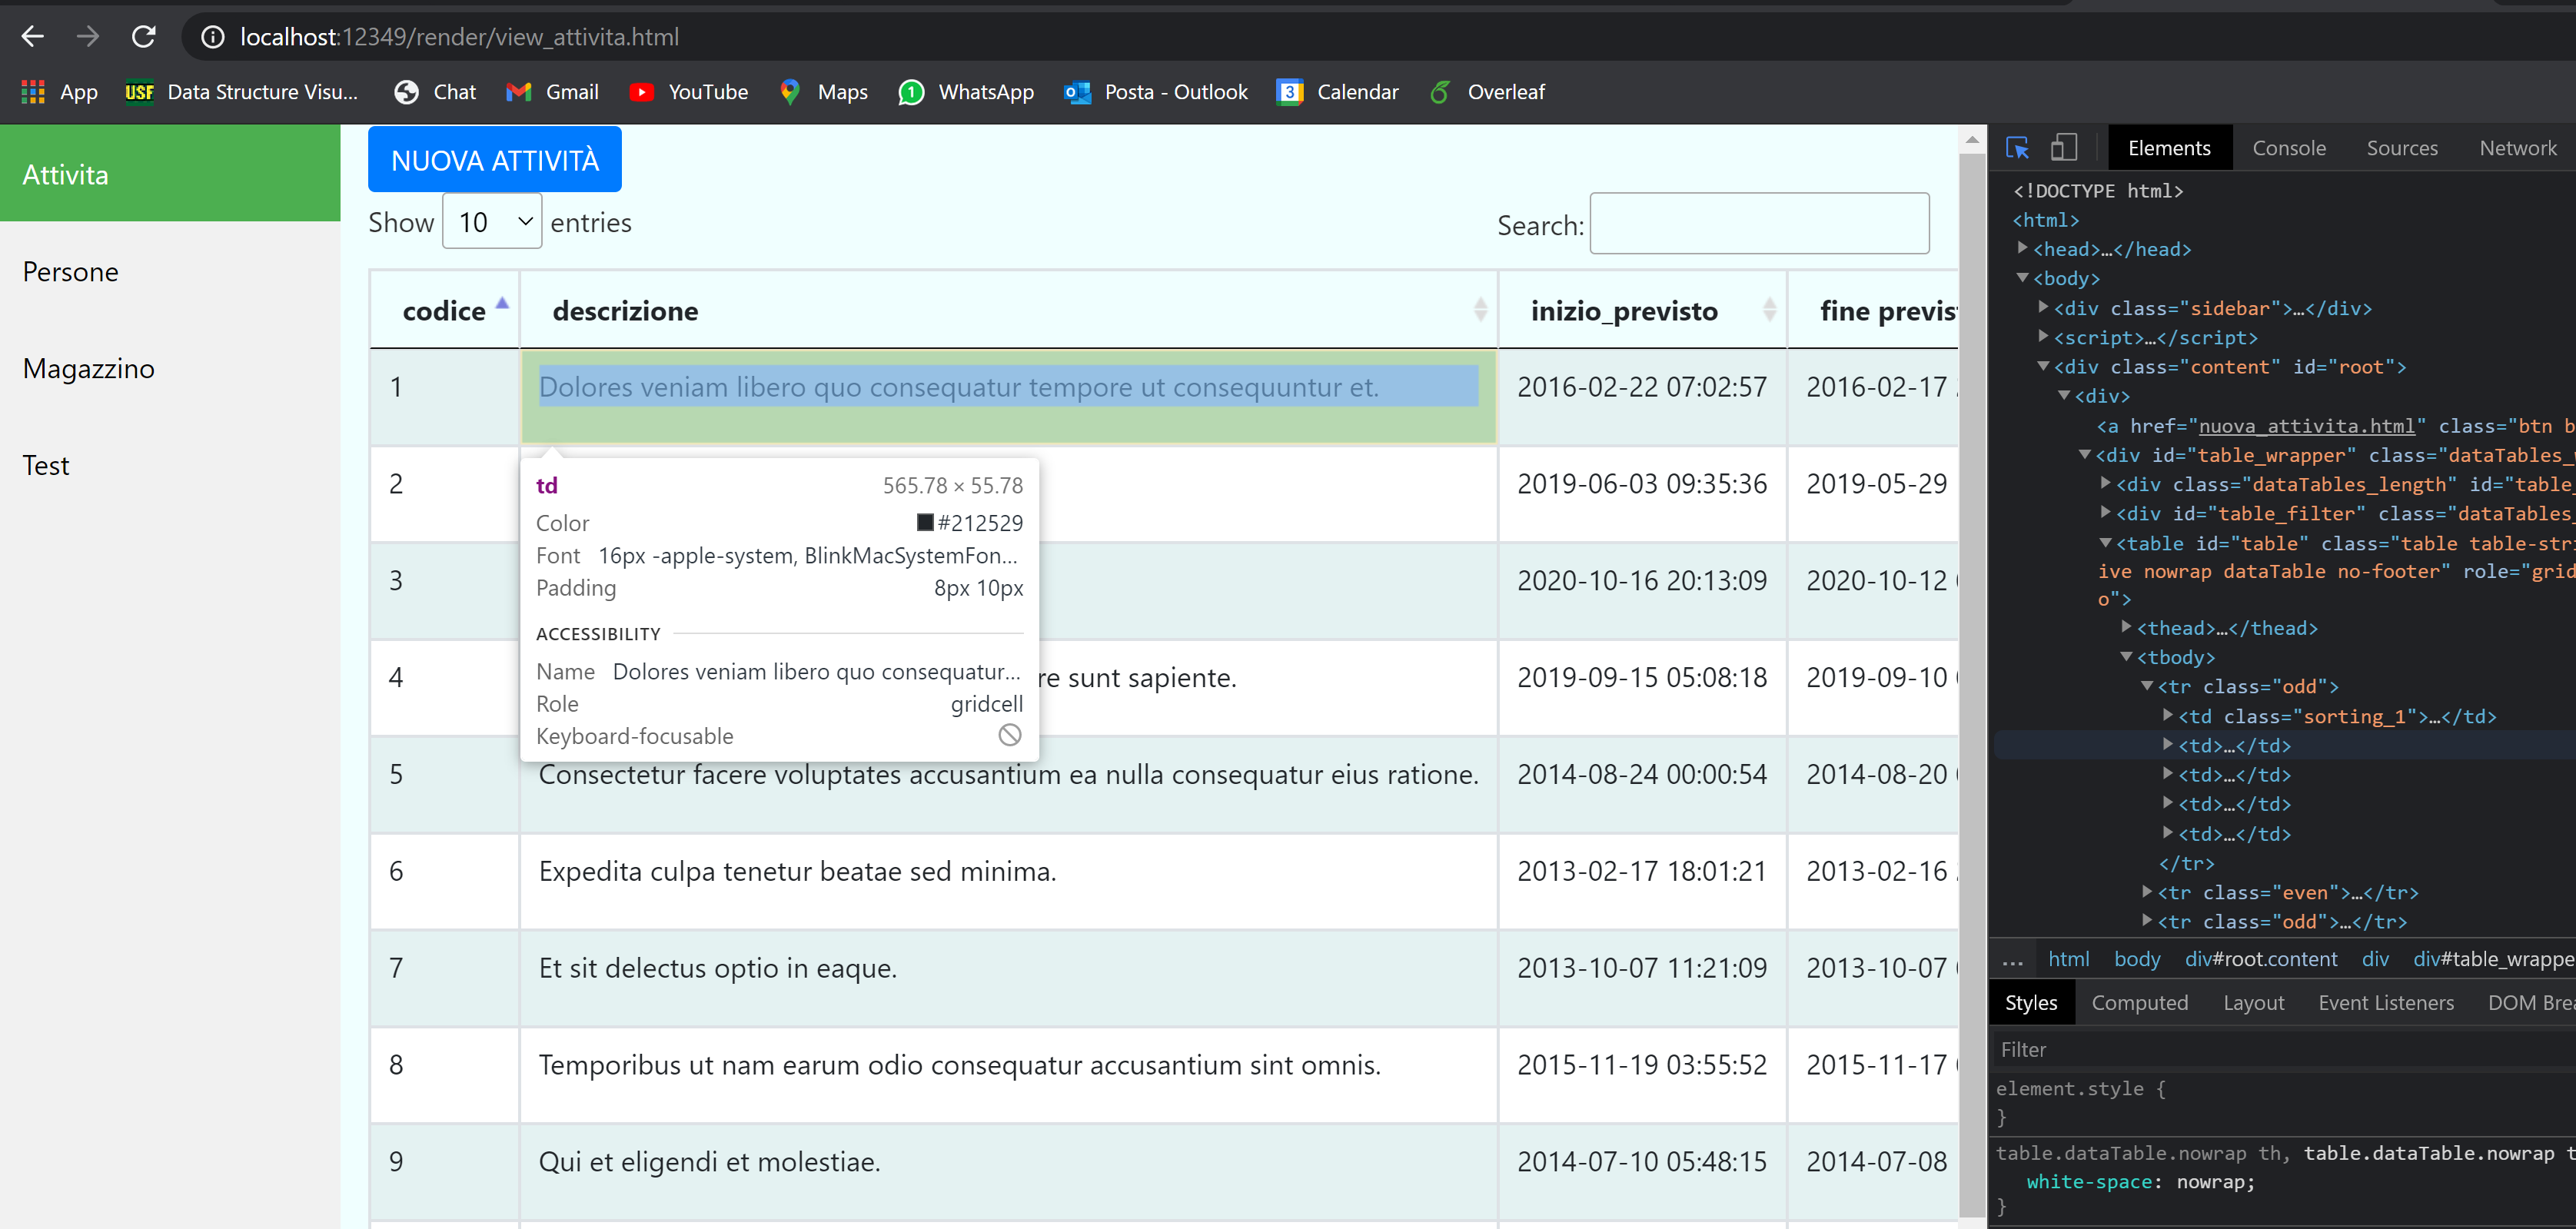
\includegraphics[width=0.8\textwidth]{img/prova_chrome.png}
    \caption{Testing con il browser \emph{Google chrome} durante lo sviluppo del website}
\end{figure}


\subsection{Deploy locale}

\paragraph{} Il deploy è stato effettuato anche questa volta tramite Docker. Sfruttando il fatto che Flask (gunicorn) è già attivo per servire le API, è conveniente includere il website all'interno del container preesistente. 

\paragraph{} Di seguito alcuni screenshot del risultato finale. 

\begin{figure}[H]
    \centering
    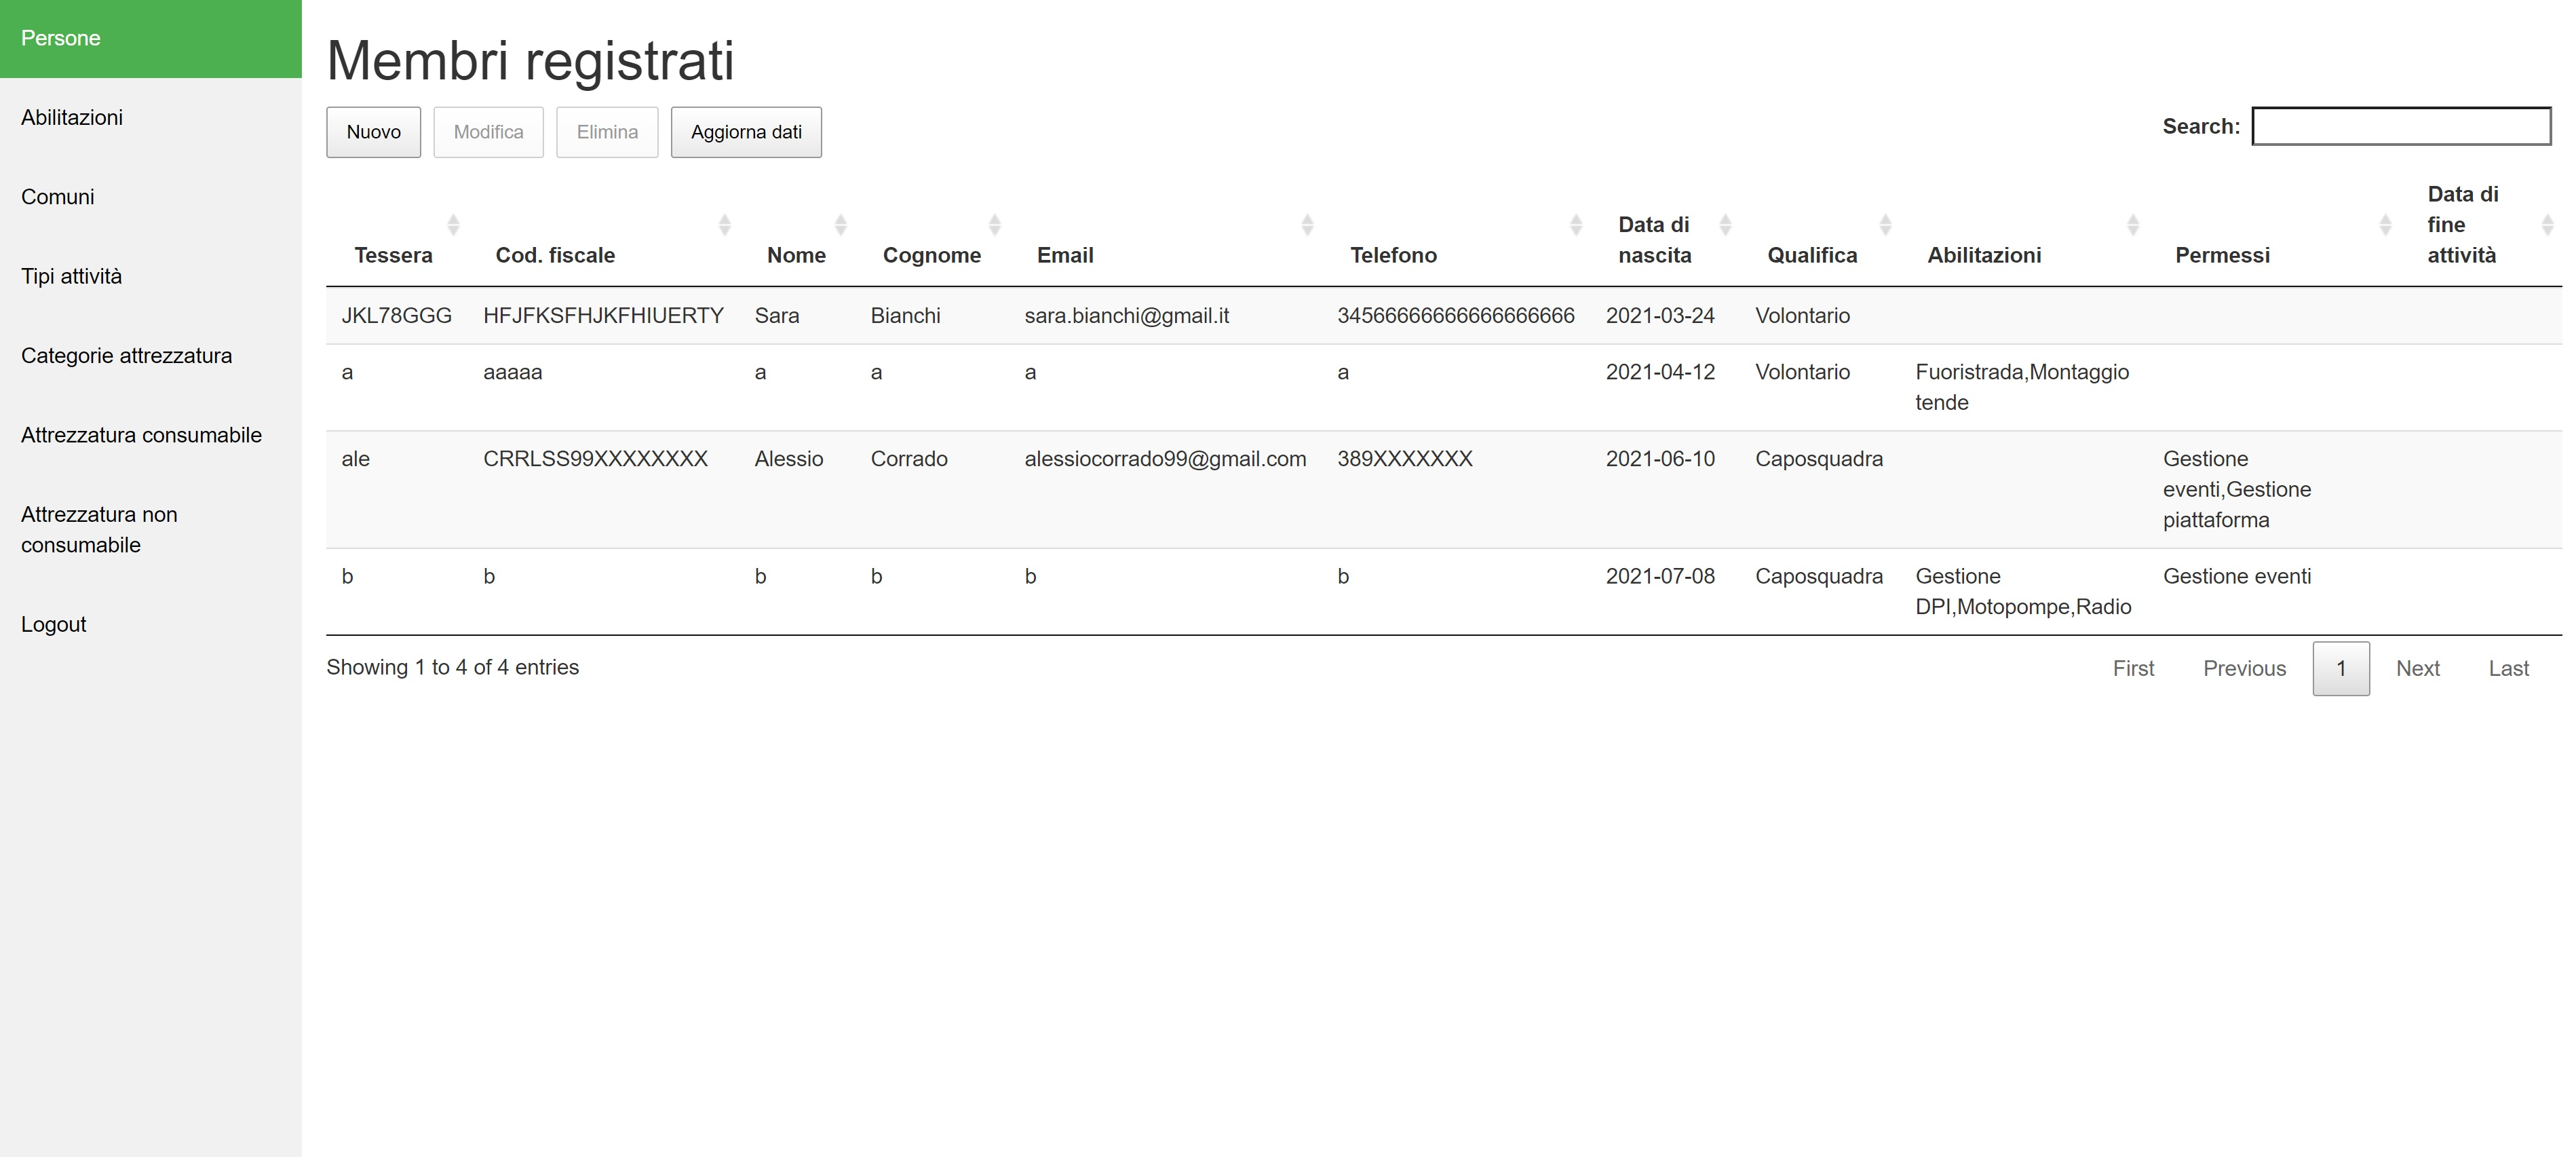
\includegraphics[width=0.8\textwidth]{img/persona.jpg}
    \caption{Persona}
\end{figure}

\begin{figure}[H]
    \centering
    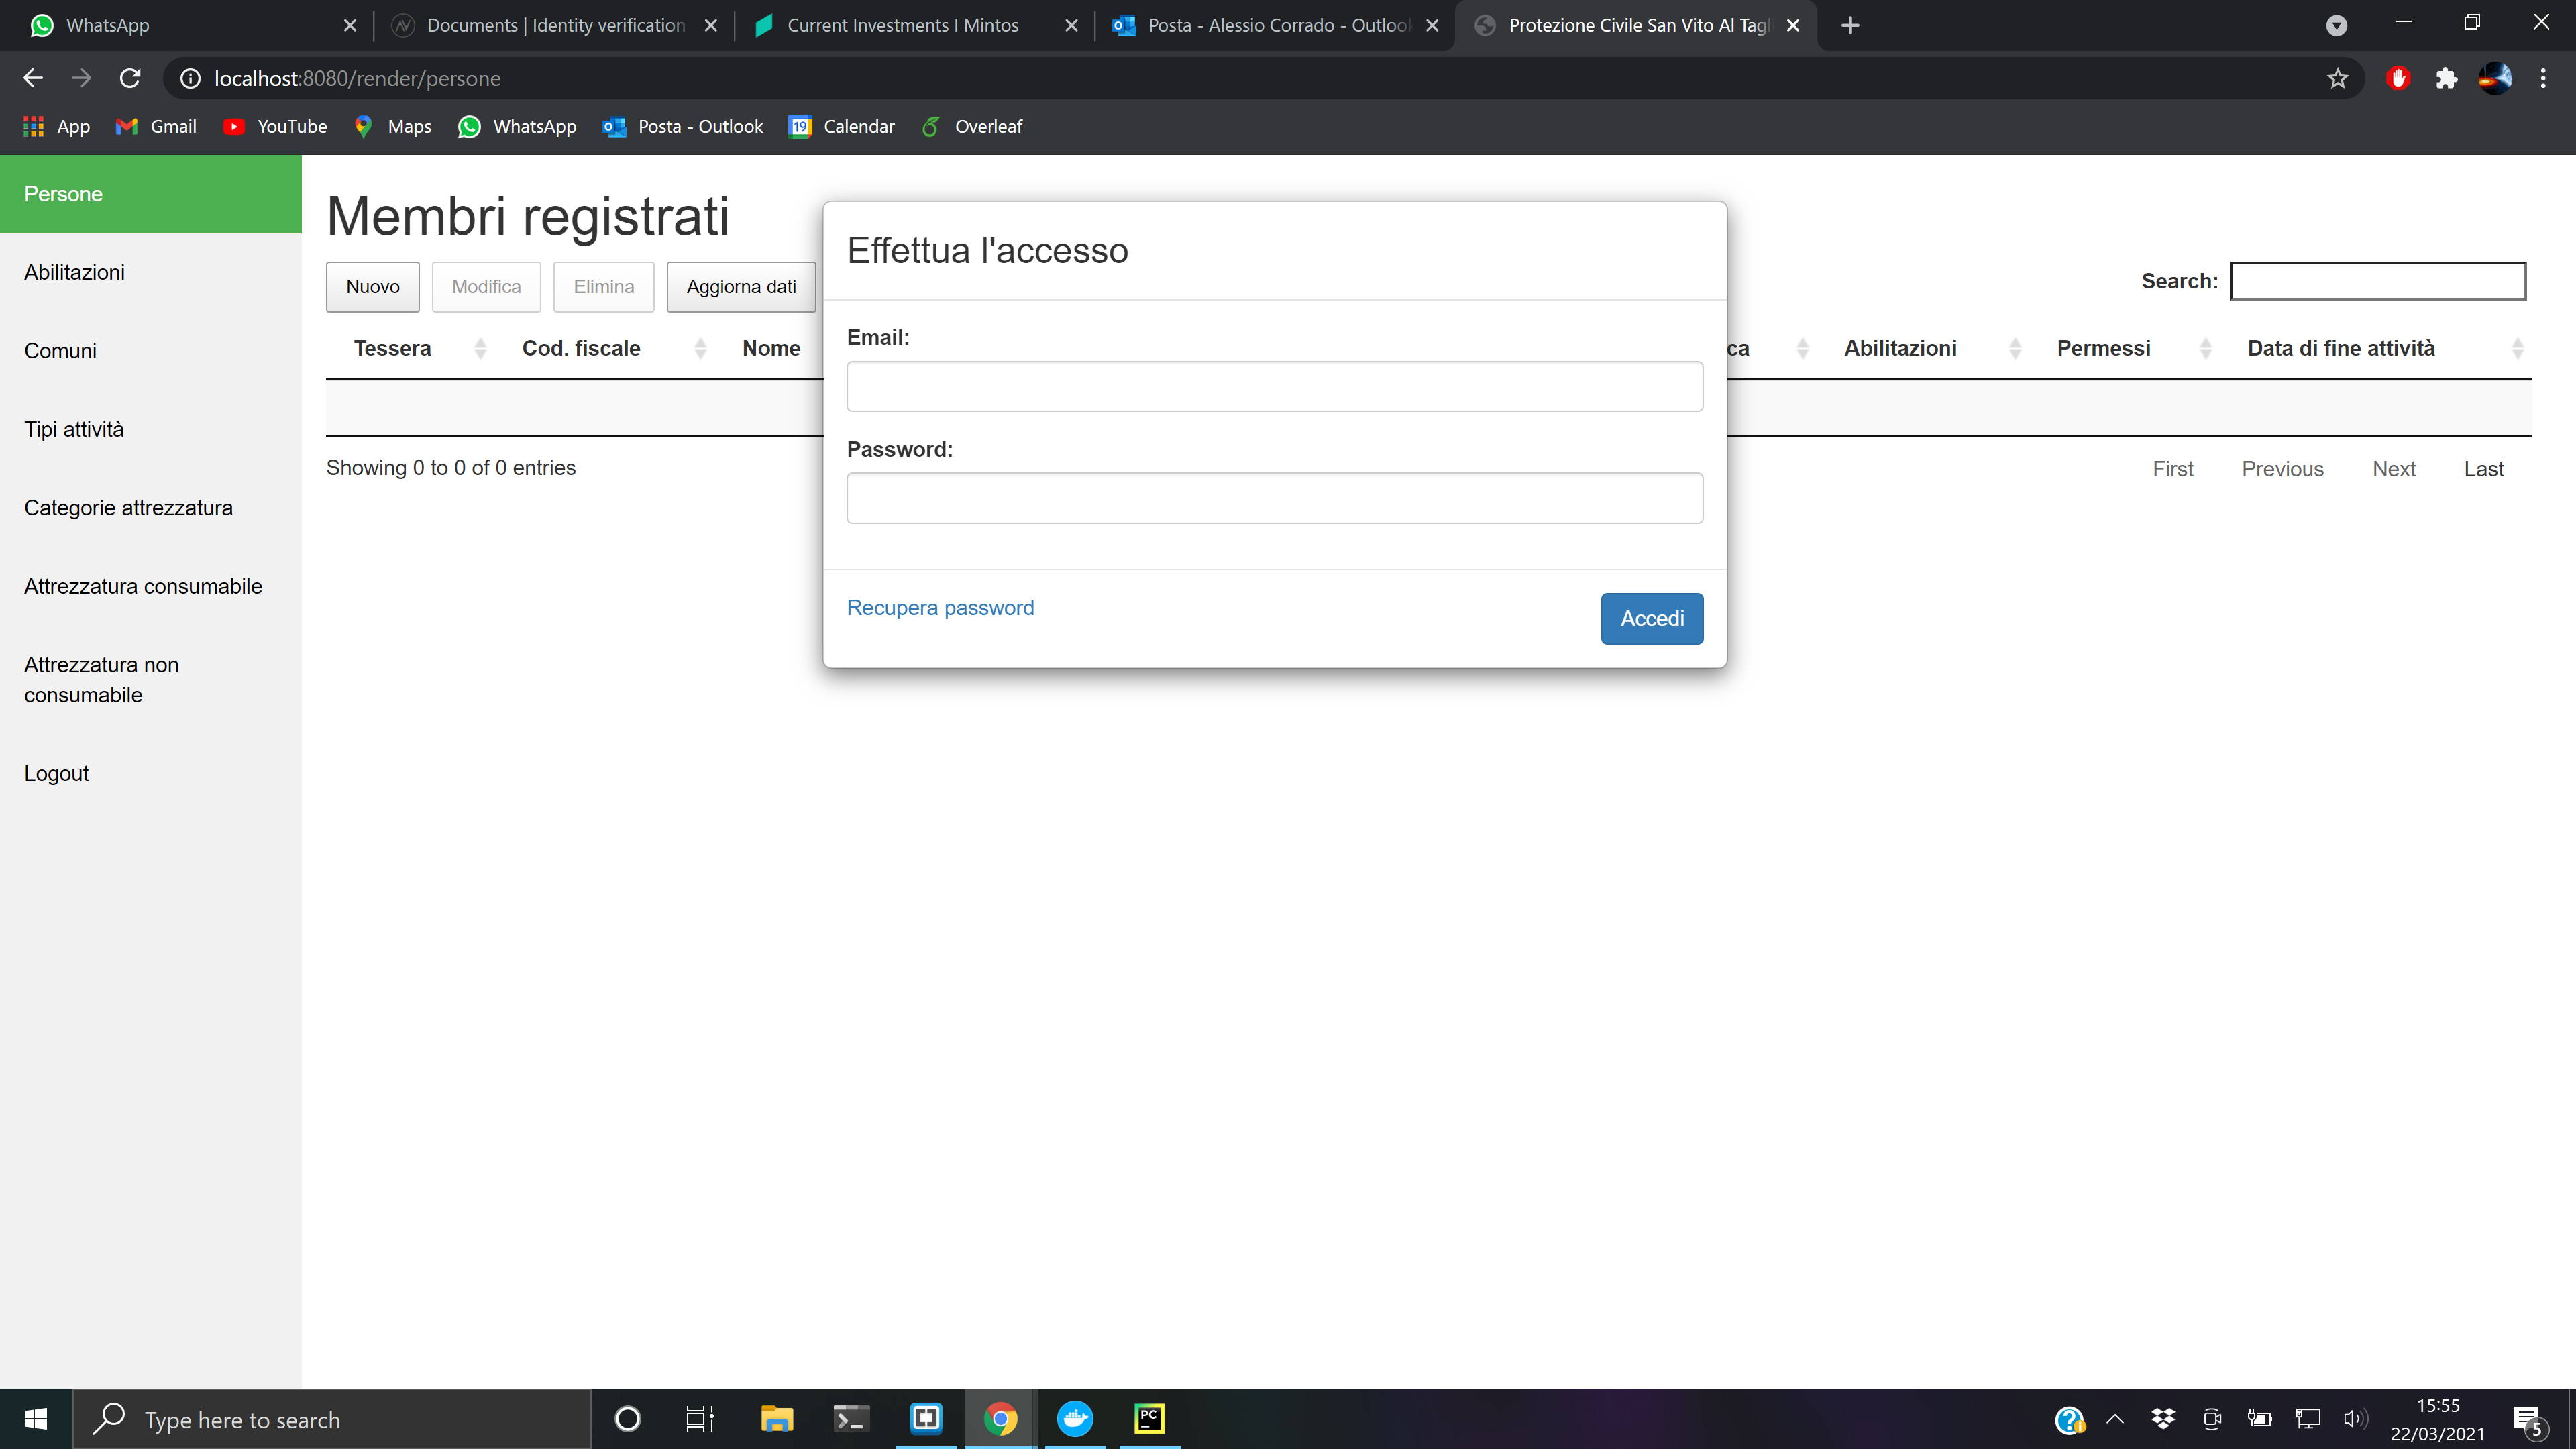
\includegraphics[width=0.8\textwidth]{img/login.png}
    \caption{Login}
\end{figure}

\begin{figure}[H]
    \centering
    \includegraphics[width=0.8\textwidth]{img/recupero_screen.jpg}
    \caption{Recupero password}
\end{figure}

\begin{figure}[H]
    \centering
    \includegraphics[width=0.8\textwidth]{img/new.png}
    \caption{Nuova persona}
\end{figure}


%\section{Analisi dei dati}
%todo analisi dei dati



\section{Deploy}

\paragraph{} Per il deploy si è scelto di utilizzare \emph{Google Cloud (GCP)}. 

\paragraph{} \emph{GCP} \cite{gcp} è la piattaforma cloud offerta da Google. Essa contiene una lunga lista di servizi, che riguardano tutti gli aspetti principali dello sviluppo in cloud.  

\paragraph{} Le principali categorie di servizi sono le seguenti:
\begin{itemize}
    \item \emph{Computing}: ciò che serve per effettuare computazioni e lanciare istanze di applicazioni;
    \item \emph{Archiviazione}: file storage persistente;
    \item \emph{Database}: storage mediante basi di dati, sia relazionali che non;
    \item \emph{Networking}: gestione delle reti tra servizi e sicurezza delle reti;
    \item \emph{Big data}: strumenti per lavorare con big data e IoT;
    \item \emph{Intelligenza artificiale}: modelli preaddestrati e strumenti per l'intelligenza artificiale;
    \item \emph{Strumenti}: strumenti vari per la costruzione di container, lo scheduling di operazioni, la gestione degli endpoint e altro ancora;
    \item \emph{Operazioni}: monitoraggio, logging, debugging e profiling dei servizi attivi.
\end{itemize}

\subsection{Deploy del database}

\paragraph{} Per il deploy del database si è scelto di utilizzare \emph{SQL}. 

\paragraph{} Esso fornisce l'accesso a istanze di database MySQL e PostgreSQL completamente gestite. Ciò vuol dire che è la piattaforma a occuparsi interamente del deploy delle instanze, del loro mantenimento, del load balancing, del backup e tutto il resto. 

\paragraph{} Considerando il carico ridotto, è stata scelta un'istanza base. Essa dispone di 1 vCPU\footnote{Le vCPU, o \emph{virtual CPU}, sono cpu virtualizzate. Più vCPU possono condividere la stessa CPU fisica.}, 3.75 GB di memoria primaria, 10 GB di memoria secondaria HDD.

\paragraph{} Un modo semplice per effettuare l'importazione dei dati è collegarsi direttamente all'istanza tramite \emph{shell psql} e importare un dump del database locale. 
\paragraph{} Per rendere i dati più sicuri, è stato attivato un backup periodico giornaliero.

\subsection{Deploy delle API e website}

\paragraph{} Per il deploy delle API e website si è scelto di usare \emph{App Engine}.

\paragraph{} App Engine fornisce un servizio di pubblicazione per webapp scritte in diversi linguaggi, tra cui Python. 

\paragraph{} È anch'esso completamente gestito: la piattaforma si occupa di costruire le istanze docker e caricarle sui server per la pubblicazione. La piattaforma fornisce anche un servizio automatico di gestione del carico, mediante il deploy temporaneo di un maggior numero di istanze. 

\paragraph{} Per pubblicare una webapp su App Engine è sufficiente richiamare i comandi appropriati tramite shell. 

\begin{lstlisting}[caption=Pubblicazione della webapp su App Engine]
gcloud app deploy
\end{lstlisting}

\paragraph{} Di default la webapp è disponibile ad un indirizzo offerto dalla piattaforma. È possibile acquistare un dominio personalizzato sempre all'interno della piattaforma.

\subsection{Pubblicazione dell'app}

\paragraph{} Per pubblicare le app Android e iOS sui relativi store, è necessario costruire delle app standalone, che non siano più legate alla piattaforma Expo. 

\paragraph{} Per farlo è sufficiente creare un file di configurazione, che istruisca Expo su come effettuare il build, e poi lanciare il comando apposito per la piattaforma. 

\begin{lstlisting}[title=Struttura del file di configurazione]
{
   "expo": {
    "name": "Your App Name",
    "icon": "./path/to/your/app-icon.png",
    "version": "1.0.0",
    "slug": "your-app-slug",
    "ios": {
      "bundleIdentifier": "com.yourcompany.yourappname",
      "buildNumber": "1.0.0"
    },
    "android": {
      "package": "com.yourcompany.yourappname",
      "versionCode": 1
    }
   }
 }
\end{lstlisting}

\begin{lstlisting}[title=Comandi per effettuare il build delle due app]
expo build:ios     

expo build:android -t app-bundle
\end{lstlisting}

\paragraph{} Una volta terminato il build e relativi test, è sufficiente accedere al profilo personale degli store e caricare quanto necessario. 


\section{Conclusioni e sviluppi futuri}

\paragraph{} Svolgere questo progetto è stato particolarmente interessante perchè esso racchiude l'applicazione di conoscenze maturate nel corso dell'intero percorso di studi triennale. 

\paragraph{} Le discipline maggiormente utilizzate sono:
\begin{itemize}
    \item \emph{Ingegneria del sotfware}: ciclo di vita del software, raccolta ed analisi dei requisiti, diagrammi di progettazione, architettura del sistema, politica di qualità, testing;
    \item \emph{Interazione uomo-macchina}: design ux/ui, user-centered design;
    \item \emph{Basi di dati}: sviluppo del database;
    \item \emph{Reti di calcolatori}: scambio di dati in rete, autenticazione e sicurezza;
    \item \emph{Programmazione}: strutturazione del codice, implementazione delle soluzioni;
    \item \emph{Sistemi operativi}: configurazione ed utilizzo di server linux-based.
\end{itemize}

\paragraph{} Il risultato è particolarmente soddisfacente, non tanto per la mera implementazione, ma per essere riusciti a portare avanti un progetto coerente e ben strutturato, nonostante la complessità non indifferente. 

\paragraph{} Parte del progetto è stato svolto in team. Ciò ha permesso un dialogo costruttivo, in particolare nelle scelte più cruciali in fase di progettazione, ma ha anche mostrato le difficoltà e divergenze del lavoro di squadra. 

\paragraph{} L'interazione con il committente è stata particolarmente positiva, con una forte propositività e disponibilità. 

\paragraph{} Allo stato attuale:
\begin{itemize}
    \item il \emph{database} è implementato, completamente testato e funzionante;
    \item l'\emph{API} è implementata e funzionante. Necessità di ulteriori test, in particolare riguardo la sicurezza;
    \item il \emph{website} è implementato e in fase di testing. Necessita della validazione conclusiva da parte del committente e di piccole correzioni di bug;  
    \item l'\emph{app} è completamente progettata ma ancora in fase di sviluppo. 
\end{itemize}

\paragraph{} Ci sono stati alcuni ritardi ma, considerando gli impegni universitari e lavorativi dei membri del gruppo, oltre che la natura totalmente gratuita del progetto, il grado di sviluppo raggiunto è valutato soddisfacente da parte di tutti. In un tempo non troppo lungo sarà possibile consegnare al committente una versione completa. 

\paragraph{} Altri possibili sviluppi, realizzabili a seguito del completamento delle attività, sono:
\begin{itemize}
    \item Utilizzare lo strumento \emph{query insights} di GCP SQL per ottimizzare le query su database;
    \item Implementare l'utilizzo di Redis sulle API;
    \item Progettare ed implementare le funzionalità mancanti dell'app;
    \item Migliorare la grafica del sito web;
    \item Effettuare ulteriori test, in particolare per quanto riguarda la sicurezza;
    \item Eseguire test di profiling per individuare i bottleneck e ridurre i tempi di risposta;
    \item Progettare test automatizzati per le future release.
\end{itemize} 


\begin{thebibliography}{99}

\bibitem{protezionecivile}
Sito web Protezione Civile San Vito al Tagliamento 
\\\url{https://www.protezionecivile.fvg.it/it/comune/san-vito-al-tagliamento}

\bibitem{modelli_sviluppo}
Software Development Life Cycle
\\\url{https://www.tutorialspoint.com/sdlc/index.htm}

\bibitem{agile_manifesto}
Agile Manifesto
\\\url{https://agilemanifesto.org/}

\bibitem{req_analysis}
What Is Requirement Analysis: Overview, Applications, Techniques and Top Tools Used
\\\url{https://www.simplilearn.com/what-is-requirement-analysis-article}

\bibitem{req_document}
Build Better Requirements Documentation: Why, Who, and How
\\\url{https://www.uxbooth.com/articles/build-better-requirements-documentation-why-who-and-how/}

\bibitem{risk_management}
Risk management
\\\url{https://searchcompliance.techtarget.com/definition/risk-management}

\bibitem{prog_architetturale}
Software Architecture \& Design
\\\url{https://www.tutorialspoint.com/software_architecture_design/index.htm}

\bibitem{rest}
RESTful Web Services
\\\url{https://www.tutorialspoint.com/restful/index.htm}

\bibitem{json}
What is JSON? A better format for data exchange
\\\url{https://www.infoworld.com/article/3222851/what-is-json-a-better-format-for-data-exchange.html}

\bibitem{dfd0}
The Context Diagram and Data Flow Diagram
\\\url{https://www.tasstudent.com/2015/10/15/the-context-diagram-and_data_flow_diagram/}

\bibitem{quality}
Software quality
\\\url{https://en.wikipedia.org/wiki/Software_quality}

\bibitem{testing}
Software testing
\\\url{https://en.wikipedia.org/wiki/Software_testing}

\bibitem{db}
Database Design – 2nd Edition
\\\url{https://opentextbc.ca/dbdesign01/}

\bibitem{postgre}
PostgreSQL: The World's Most Advanced Open Source Relational Database
\\\url{https://www.postgresql.org/}

\bibitem{docker}
Docker
\\\url{https://www.docker.com/}

\bibitem{pgadmin}
pgAdmin
\\\url{https://www.pgadmin.org/}

\bibitem{restapi}
Understanding And Using REST APIs
\\\url{https://www.smashingmagazine.com/2018/01/understanding-using-rest-api/}

\bibitem{redis}
Redis
\\\url{https://redis.io/}

\bibitem{python}
Python
\\\url{https://www.python.org/}

\bibitem{git}
Git
\\\url{https://git-scm.com/}

\bibitem{wsgi}
Web Server Gateway Interface
\\\url{https://en.wikipedia.org/wiki/Web_Server_Gateway_Interface}

\bibitem{flask}
Flask
\\\url{https://flask.palletsprojects.com/en/2.0.x/}

\bibitem{password}
Password Authentication: Avoiding 4 Common Vulnerabilities
\\\url{https://swoopnow.com/password-authentication/}

\bibitem{insomnia}
Insomnia
\\\url{https://insomnia.rest/}

\bibitem{design}
App Design Process: How to Design a Great Mobile App
\\\url{https://www.iteratorshq.com/blog/app-design-process-design-a-great-mobile-app/}

\bibitem{ucd}
User-Centered Design: Process and Benefits
\\\url{https://uxplanet.org/user-centered-design-process-and-benefits-fd9e431eb5a9}

\bibitem{react_n}
React Native
\\\url{https://reactnative.dev/}

\bibitem{expo}
Expo
\\\url{https://expo.io/}

\bibitem{frontend_vs_backend}
What's The Difference Between Frontend And Backend Web Development?
\\\url{https://careerfoundry.com/en/blog/web-development/whats-the-difference-between-frontend-and-backend/}

\bibitem{jinja}
Jinja
\\\url{https://jinja.palletsprojects.com/en/3.0.x/}

\bibitem{ajax}
Ajax calls
\\\url{https://en.wikipedia.org/wiki/Ajax_(programming)}

\bibitem{bootstrap}
Boostrap
\\\url{https://getbootstrap.com/}

\bibitem{jquery}
jQuery
\\\url{https://jquery.com/}

\bibitem{gcp}
Google Cloud Platform
\\\url{https://cloud.google.com/}


\end{thebibliography}

\end{document}
